\documentclass[sigconf]{acmart}

\settopmatter{printacmref=false}
\renewcommand\footnotetextcopyrightpermission[1]{}
\pagestyle{plain}

%Course information
\acmConference
[CSE 6275/CSE 6391: AHCI, Assignment 2]
{}
{CSE Dept.}
{IUT}

\usepackage[utf8]{inputenc}
\usepackage{microtype}
\usepackage{graphicx}
\setlength{\emergencystretch}{2em}
\usepackage{booktabs}
\usepackage{multirow}
\usepackage{enumitem}
\usepackage{array}
\usepackage{hyperref}
\usepackage{tcolorbox}
\tcbuselibrary{breakable}
\usepackage{float}
% \usepackage{fontspec}

% Color definitions matching the DrowsyGuard design system
\definecolor{teal}{HTML}{0D9488}
\definecolor{navy}{HTML}{0F172A}
\definecolor{coral}{HTML}{E8571A}
\definecolor{promptbg}{HTML}{F8FAFC}
\definecolor{promptframe}{HTML}{0D9488}

% Prompt box style for Lovable AI prompts
   \newtcolorbox{promptbox}[1][]{
       colback=promptbg,
       colframe=promptframe,
       fonttitle=\bfseries\small,
       title={#1},
       boxrule=0.8pt,
       arc=3pt,
       left=6pt, right=6pt, top=4pt, bottom=4pt,
       fontupper=\small,
       breakable
   }


\title{Human-Centered AI for Driver Drowsiness Detection: Design and Prototype Development}


\author{Sadik Yasin Eftee}
\affiliation{
  \institution{Department of Computer Science and Engineering\\
  Islamic University of Technology (IUT), OIC}
  \city{Dhaka}
  \country{Bangladesh}
}
\email{sadikyasin@iut-dhaka.edu}

\author{Abdullah Al Mamun}
\affiliation{
  \institution{Department of Computer Science and Engineering\\
  Islamic University of Technology (IUT), OIC}
  \city{Dhaka}
  \country{Bangladesh}
}
\email{mamun24@iut-dhaka.edu}

\author{Md Tasriful Islam}
\affiliation{
  \institution{Department of Computer Science and Engineering\\
  Islamic University of Technology (IUT), OIC}
  \city{Dhaka}
  \country{Bangladesh}
}
\email{tasriful@iut-dhaka.edu}


\author{Nazifa Mim}
\affiliation{
  \institution{Department of Computer Science and Engineering\\
  Islamic University of Technology (IUT), OIC}
  \city{Dhaka}
  \country{Bangladesh}
}
\email{nazifacse1@gmail.com}

\author{Hasan Mahmud}
\affiliation{
  \institution{SSL, Department of Computer Science and Engineering\\
  Islamic University of Technology (IUT), OIC}
  \city{Dhaka}
  \country{Bangladesh}
}
\email{hasan@iut-dhaka.edu}

\authornote{Hasan Mahmud.}

\begin{document}

\begin{abstract}

Driver drowsiness remains a leading cause of road accidents, yet existing detection systems largely neglect the human interaction dimension---providing opaque, one-size-fits-all interfaces that fail to account for the diverse needs, technology literacy levels, and cultural contexts of real-world drivers. This work presents the design, construction, and formative evaluation of a Human-Centered AI (HCAI) driver drowsiness detection system comprising three persona-driven prototype variants and a unified mode-switching architecture, grounded in empirical survey data collected from 11 Bangladeshi professional drivers (truck, bus, and private car operators).
 
A 60-question survey across 8 thematic blocks revealed that drivers unanimously prioritized detection accuracy (mean 4.82/5), strongly preferred Bangla plain-language explanations over technical metrics (4.73/5), had zero prior experience with any driver monitoring system, universally preferred on-device data processing, and were divided in their interface complexity preferences---45\% favoring simple companion-style interfaces, 36\% moderate dashboards, and 18\% data-rich technical displays. These findings motivated a persona-driven multi-variant design approach rather than a single averaged interface.
 
Three functional prototypes were built using Lovable AI from carefully engineered build prompts treated as formal design specifications: (1)~DrowsyGuard, a status-focused dashboard with bilingual alerts; (2)~Saathi, a conversational companion using an animated character for non-tech-savvy drivers; and (3)~DrowsyHUD, a data-rich heads-up display exposing real-time detection metrics. A requirements traceability analysis across all three variants revealed that no single design achieved complete coverage of the identified requirements, motivating a fourth unified prototype---a mode-switching application that consolidates all three interaction paradigms within a single deployable system with a shared detection engine, state-preserving mode transitions, and cross-mode features including smart break reminders and emergency contact escalation.
 
Formative evaluation through requirements traceability, HCAI principle compliance audit, and scenario-based walkthroughs confirmed that the unified prototype achieves full coverage across all 14 traced requirements and complete HCAI compliance through complementary mode-specific implementations. The unified design was subsequently realised as a deployable Android application (Expo SDK~55, React Native) with real on-device Google ML Kit face detection replacing the simulation engine, and evaluated with a private commuter cohort ($n$~=~3). The evaluation yielded a mean System Usability Scale score of 78.3, mean NASA Task Load Index of 2.39/10 (very low cognitive load), mean trust rating of 4.25/5, mean Net Promoter Score of 8.0, and unanimous stated intent to install the application. A key contribution is the demonstration that HCAI principles of transparency, explainability, reliability, and human oversight are implementation-agnostic: a low-literacy truck driver receiving AI assistance through an animated companion's emotional expressions and a tech-savvy private driver receiving the same assistance through real-time metric gauges both experience HCAI-compliant interaction---calibrated to their needs through fundamentally different interface paradigms serving the same safety objective.

\end{abstract}

\keywords {Human-Centered AI, Driver Drowsiness Detection, Facial Landmarks, Requirements Engineering, Personas, Scenario-Based Design, Interaction Design}

\maketitle


\section{Introduction}

\subsection{Background and Motivation}

Drowsy driving poses a serious global road safety risk, contributing each year to a significant number of fatalities and severe injuries. Major transportation and health authorities such as the National Highway Traffic Safety Administration (NHTSA) and the World Health Organization (WHO) have emphasized the urgency of addressing this preventable issue \cite{ref1}. Studies report that drowsiness-related crashes account for thousands of accidents annually, highlighting the need for effective monitoring and early-warning systems \cite{ref2, ref3}.

Recent advancements have led to Driver Drowsiness Detection (DDD) systems that assess alertness through physiological signal monitoring \cite{ref4}, vehicle driving pattern analysis \cite{ref5}, and vision-based facial feature analysis \cite{ref6, ref8}. Among these, facial landmark-based methods are particularly attractive because they are non-intrusive, require minimal setup, and enable real-time detection using standard cameras \cite{ref9}. Multimodal approaches combining multiple fatigue cues have shown improved robustness \cite{ref10}.

However, a critical gap exists between detection technology and driver experience. Most existing systems focus almost exclusively on improving detection accuracy while neglecting the \textit{human interaction} dimension: How should a drowsiness alert be communicated to a truck driver with limited technology experience? How much technical detail should be shown to a data-savvy private car driver? How can a monitoring system build trust with users who have never encountered such technology? These questions are fundamentally Human-Centered AI (HCAI) design challenges \cite{ref14}, yet the existing literature offers little guidance on how to design drowsiness detection interfaces that account for diverse user needs, cultural contexts, and technology literacy levels.

This gap is especially acute in the Bangladeshi context, where professional drivers face severe fatigue risks---our survey found that 82\% experience drowsiness weekly and 73\% have had drowsiness-related safety incidents---yet 100\% have zero prior exposure to any driver monitoring system. Designing for this population requires not only accurate detection but also culturally appropriate, trustworthy, and accessible interface design grounded in empirical user research.

\subsection{From Requirements to Design}

This work builds directly on a prior formative requirements analysis, where the primary stakeholders, user needs, and system requirements were established through a user-centered analysis. The current study translates those requirements into functional prototype designs through a structured four-phase process:

\begin{enumerate}
    \item \textbf{User Research:} A 60-question survey administered to 11 Bangladeshi professional drivers (the primary stakeholders) to understand drowsiness experience, technology attitudes, privacy concerns, and interface preferences.
    \item \textbf{Persona-Driven Variant Design:} Development of three distinct user personas from survey data, each mapped to a separate prototype variant built using Lovable AI with formally specified build prompts.
    \item \textbf{Formative Evaluation:} Requirements traceability analysis across all three variants, identifying coverage gaps and per-variant strengths.
    \item \textbf{Design Unification:} Merging the three variants into a single mode-switching application that preserves each variant's strengths while addressing coverage gaps.
\end{enumerate}

\paragraph{Primary Stakeholders (Targeted in This Study)}
All user research, survey data collection, persona development, and prototype evaluation were conducted exclusively with the primary stakeholders---the drivers themselves:

\begin{itemize}
    \item Professional truck drivers
    \item Intercity bus drivers
    \item Private car drivers
\end{itemize}

While secondary stakeholders (transportation companies, road safety authorities, vehicle manufacturers) may benefit from the system in future work, the current study focuses exclusively on understanding and designing for the direct end-users in safety-critical driving contexts.

\paragraph{Key Requirements from the Formative Analysis}
The following functional and non-functional requirements, established during the initial requirements engineering phase, guided the prototype design:

\begin{table}[h]
\centering
\caption{Key Requirements Guiding the Prototype Design}
\begin{tabular}{|p{3cm}|p{5cm}|}
\hline
\textbf{Requirement} & \textbf{Description} \\
\hline
Facial Monitoring & Detect driver face and track facial landmarks using a camera-based system. \\
\hline
Eye Closure Detection & Measure Eye Aspect Ratio (EAR) to identify prolonged eye closure. \\
\hline
Yawning Detection & Detect yawning as an additional fatigue indicator. \\
\hline
Head Pose Monitoring & Monitor head position to detect abnormal tilting or nodding. \\
\hline
Alert Mechanism & Provide real-time audio or visual alerts when drowsiness is detected. \\
\hline
Usability & Interface should be simple, intuitive, and non-distracting. \\
\hline
Privacy & Camera data should be processed locally to protect user privacy. \\
\hline
Explainability & Alerts should explain why drowsiness was detected, in the driver's language. \\
\hline
\end{tabular}
\end{table}

\subsection{Objectives and Contributions}

The objective of this study is to design, build, and evaluate functional prototypes for a Human-Centered AI driver drowsiness detection system. Rather than a single monolithic design, this work proposes a persona-driven multi-variant approach that explicitly addresses the diverse needs of the primary stakeholder population.

The key contributions include:

\begin{itemize}
    \item A 60-question survey analysis of 11 Bangladeshi professional drivers (primary stakeholders), producing six publication-quality data visualizations that establish the empirical basis for design decisions.
    \item Three distinct user personas (Rahim, Karim, Fatema) derived from survey data clusters, representing low, moderate, and high technology literacy levels.
    \item Three functional prototypes built via Lovable AI from formally specified build prompts: DrowsyGuard (Dashboard), Saathi (Companion), and DrowsyHUD (Technical HUD), each with live deployments.
    \item A requirements traceability analysis across all three variants demonstrating HCAI principle coverage and identifying design gaps.
    \item An evaluation-driven unification into a single mode-switching architecture, with rationale for why no single design suffices for the diverse primary stakeholder population.
    \item Demonstration that HCAI principles (transparency, explainability, reliability, human oversight) can be realized at multiple levels of interface complexity---from a conversational companion to a data-rich dashboard.
\end{itemize}

\section{Related Work and Design Inspirations}

\subsection{Drowsiness Detection Approaches}

Research on Driver Drowsiness Detection (DDD) has advanced significantly through computer vision, machine learning, and deep learning techniques. Modern systems primarily analyze facial behaviors---eye closure, blink frequency, yawning, and head pose---to provide non-intrusive, real-time monitoring~\cite{ref3, ref6}. Comprehensive reviews of sensor-based approaches~\cite{ref24} and behavioral measure methods~\cite{ref28} confirm that vision-based facial analysis has become the dominant paradigm due to its non-intrusiveness and accuracy.

Hussain and Kim~\cite{ref1} developed a real-time CNN--RNN architecture for eye-state classification, achieving approximately 97\% accuracy. Patel and Singh~\cite{ref2} proposed a CNN-based approach for eye state classification under varying lighting conditions with over 95\% accuracy and low latency. Zhang and Wang~\cite{ref3} introduced a multimodal framework combining PERCLOS, facial landmarks, and Random Forest classification, reporting approximately 90\% accuracy under head movement variations. Rim et al.~\cite{ref8} reviewed physiological signal approaches (EEG, ECG), finding high accuracy but limited real-world adoption due to intrusive sensors. Ramzan et al.~\cite{ref25} provide a comprehensive survey of state-of-the-art techniques, confirming that eye-closure metrics (PERCLOS and EAR) remain the most reliable single indicators across detection paradigms. Hu and Zheng~\cite{ref21} demonstrated SVM-based eyelid parameter classification achieving strong drowsiness detection, while Vural et al.~\cite{ref22} showed that multi-feature facial analysis outperforms single-cue approaches in automated drowsiness assessment.

\subsection{The Interface Design Gap}

While detection accuracy has improved dramatically, a significant gap persists in how these systems \textit{communicate} with drivers. Our review of the literature reveals three critical interface design shortcomings:

\textbf{One-size-fits-all interfaces.} Existing systems provide a single alert modality and interface design, ignoring the wide variation in driver technology literacy, language preferences, and information needs. Our survey confirmed this variation: 45\% of Bangladeshi drivers preferred simple companion-style interfaces while 18\% wanted detailed technical dashboards.

\textbf{Lack of cultural and linguistic adaptation.} Most DDD interfaces are designed for English-speaking, technology-literate Western users. Our survey found that Bangla plain-language explanation was the highest-priority feature (4.73/5), yet no existing system provides native-language conversational explanations for South Asian drivers.

\textbf{Insufficient HCAI compliance.} Table~\ref{tab:approaches} summarizes how existing paradigms fall short of HCAI principles. Traditional ML systems offer interpretable features but no natural-language explanations. Deep learning systems achieve high accuracy but remain opaque. Even emerging VLM approaches, while capable of natural-language output, lack the real-time performance and user-centered interface design needed for deployment.

\begin{table}[H]
\caption{Comparison of drowsiness detection paradigms and their HCAI implications.}
\label{tab:approaches}
\small
\setlength{\tabcolsep}{3pt}
\begin{tabular}{p{1.3cm}p{1.9cm}p{1.0cm}p{2.2cm}}
\toprule
\textbf{Paradigm} & \textbf{Methods} & \textbf{Acc.} & \textbf{HCAI Gap}\\
\midrule
Traditional ML & SVM, RF, KNN; EAR, PERCLOS & 84--99\% & Interpretable features; binary output; no explanation text\\[3pt]
Deep Learning & CNN, CNN-LSTM, ViT; end-to-end & 93--99\% & High accuracy; opaque; no natural language\\[3pt]
VLMs & CLIP, GPT-4V, LLaVA & 51--64\% & Slow; costly; strong natural-language output\\
\bottomrule
\end{tabular}
\end{table}

\subsection{Motivation for a Multi-Variant HCAI Approach}

Motivated by these gaps, our work shifts the focus from detection accuracy to \textit{interface design for human-AI interaction in drowsiness detection}. Rather than improving the underlying ML model, we investigate how the same detection output can be communicated through different interface paradigms to serve different user personas. This approach is inspired by Shneiderman's framework for Human-Centered AI \cite{ref14}, which argues that AI systems must balance automation with human oversight, and by interaction design principles emphasizing that understanding users and their context is essential before developing interactive systems \cite{ref12, ref13}.

Our specific contributions to closing the interface design gap are: (a)~conducting user research with the actual target population (Bangladeshi professional drivers), (b)~deriving distinct personas from empirical data rather than assumptions, (c)~building multiple functional prototypes rather than a single design, and (d)~evaluating these designs against HCAI principles before unifying them.

\section{Design Goals and HCAI Principles}

Since the proposed system operates in a safety-critical driving context, the prototype design must satisfy not only technical detection requirements but also usability, trust, and HCAI compliance goals. These goals were refined based on the survey findings from the primary stakeholders.

\subsection{Usability Goals}

The survey data revealed that Bangladeshi drivers---many with limited technology experience---require interfaces that are immediately understandable and minimally distracting. The following usability goals were established:

\begin{itemize}
    \item \textbf{Effectiveness:} The system should accurately detect early signs of drowsiness and provide alerts that drivers can act upon. The survey ranked accuracy as the \#1 priority.
    \item \textbf{Efficiency:} Detection and warning must operate in real time with minimal delay. Alerts must be processable with a single glance or tap, especially during active driving.
    \item \textbf{Learnability:} With 100\% of respondents having zero prior DMS experience, the interface must be intuitive enough to use without training. The Companion Mode (Saathi) was specifically designed to address this by using a conversational metaphor.
\end{itemize}

\subsection{User Experience Goals}

Beyond basic usability, the prototype must promote a supportive and trustworthy driving experience that respects the primary stakeholders' cultural context:

\begin{itemize}
    \item \textbf{Trust Building:} With zero prior DMS experience among all respondents, trust cannot be assumed---it must be built. The design addresses this through privacy assurance badges, the Saathi companion character, confidence percentages, and Fitzpatrick fairness certification.
    \item \textbf{Cultural Sensitivity:} The Bangladeshi driving context includes informal coping strategies (betel leaf, face splashing), family-oriented safety motivation, and the importance of Bangla-language communication. The Companion Mode explicitly incorporates these cultural elements.
    \item \textbf{Sense of Control:} The survey confirmed that drivers want to remain the final decision-maker. All three prototype variants provide dismiss, false alarm flagging, and voluntary rest stop navigation---never autonomous action.
    \item \textbf{Reduced Anxiety:} Alerts are designed to be calm and non-intrusive. The Companion Mode uses warm colors and conversational language; the Dashboard uses simple color-coded states; the HUD provides data without panic-inducing framing.
\end{itemize}

\subsection{Human-Centered AI Principles}

The prototype design follows the four core HCAI principles identified by Shneiderman \cite{ref14}. Critically, our design demonstrates that each principle can be implemented at \textit{multiple levels of interface complexity}, allowing different user personas to experience the same HCAI guarantees through different interaction paradigms:

\begin{table}[h]
\centering
\caption{HCAI Principles Implemented Across Three Complexity Levels}
\label{tab:hcai_features}
\small
\begin{tabular}{|p{1.5cm}|p{2cm}|p{2cm}|p{2cm}|}
\hline
\textbf{Principle} & \textbf{Companion (Simple)} & \textbf{Dashboard (Moderate)} & \textbf{HUD (Detailed)} \\
\hline
Transparency & Character expression encodes state & Color-coded status indicator & All metrics visible in real time \\
\hline
Explainability & ``Your eyes are getting heavy'' (Bangla) & Bangla + English + confidence \% & Exact values with thresholds \\
\hline
Reliability & Multiple cues behind character logic & Composite status from multiple cues & All cues independently visible \\
\hline
Human Oversight & Dismiss, flag, rest (single-tap) & Dismiss, flag, rest, weekly review & Dismiss, flag, export, heatmap \\
\hline
\end{tabular}
\end{table}

This multi-level approach to HCAI compliance is a key contribution: it shows that a low-literacy truck driver and a tech-savvy private driver can both receive transparent, explainable, reliable, and human-controlled AI assistance---through fundamentally different interfaces calibrated to their needs.


\section{Conceptual Design of the System}

\subsection{System Overview}
The proposed system is a Human-Centered AI driver drowsiness detection prototype that assists drivers in identifying early signs of fatigue. Rather than a single interface, the system is architected as a \textbf{mode-switching application} with three distinct presentation layers---Companion, Dashboard, and HUD---sharing a common detection engine and alert logic. This architecture emerged from the evaluation finding that no single design satisfied all three primary stakeholder personas.

The system operates using a camera-based monitoring approach that analyses facial features (eye closure, head movements) through on-device AI detection. In the web prototype, detection is simulated for formative evaluation purposes; the final mobile application (Section~11) uses Google ML Kit face detection running entirely on the device.

\paragraph{Key Functionalities}
\begin{itemize}
    \item Real-time monitoring of the driver's face using a camera (simulated)
    \item Detection of eye closure using Eye Aspect Ratio (EAR)
    \item Identification of yawning behavior
    \item Head pose monitoring to detect abnormal tilting or nodding
    \item Composite fatigue scoring combining PERCLOS (40\%), blink rate (25\%), head pose (20\%), and driving duration (15\%)
    \item Bilingual (Bangla + English) real-time alerts with configurable severity levels
    \item Three switchable interface modes matching three user personas
    \item Privacy-first architecture with on-device processing
\end{itemize}

\paragraph{Primary Stakeholder User Groups}
The prototype is designed exclusively for the primary stakeholders identified during the requirements engineering phase:
\begin{itemize}
    \item Professional truck drivers (Persona: Rahim --- low tech, Companion Mode)
    \item Intercity bus drivers (Persona: Karim --- moderate tech, Dashboard Mode)
    \item Long-distance private car drivers (Persona: Fatema --- high tech, HUD Mode)
\end{itemize}

\subsection{Conceptual Model}

The conceptual model describes how drivers understand and interact with the system. The system is designed as a monitoring assistant that runs automatically in the background---the driver does not manually interact with it during normal operation. When fatigue indicators are detected, the system notifies the driver through mode-appropriate feedback: a character emotion change (Companion), a status indicator shift (Dashboard), or a metric threshold alert (HUD).

Conceptual models help users build accurate mental models of system behavior, enabling appropriate trust calibration \cite{ref12, ref13}.

\begin{table}[h]
\centering
\caption{Conceptual Model Components and Their Mode-Specific Rendering}
\small
\begin{tabular}{|p{1.5cm}|p{2cm}|p{1.7cm}|p{1.7cm}|}
\hline
\textbf{Component} & \textbf{Companion} & \textbf{Dashboard} & \textbf{HUD} \\
\hline
Camera Input & Hidden & Hidden & Recording dot visible \\
\hline
AI Detection & Drives character emotion & Drives status color & All metrics shown \\
\hline
Fatigue Eval. & Character worry level & Teal/amber/red state & Composite score \% \\
\hline
Alert & Speech bubble from Saathi & Slide-up card & Full-screen overlay \\
\hline
Driver Action & Dismiss / rest (2 buttons) & Dismiss / rest / flag & Acknowledge / flag / export \\
\hline
\end{tabular}
\end{table}

\subsection{Human--AI Interaction Model}

The Human--AI interaction follows a five-step process consistent across all three modes:

\begin{enumerate}
    \item The camera captures the driver's face during driving.
    \item The AI model analyzes facial landmarks and behavioral indicators.
    \item The system evaluates whether drowsiness indicators exceed thresholds, using a composite fatigue score.
    \item If drowsiness is detected, the system generates a mode-appropriate alert with a Bangla explanation.
    \item The driver interprets the alert and decides how to respond---the system never takes autonomous action.
\end{enumerate}

This interaction model ensures that AI acts as a supportive assistant rather than an autonomous controller, which aligns with the principles of Human-Centered AI \cite{ref14}. The key design decision is that the same five-step process produces different \textit{presentations} depending on the active mode, but the underlying detection logic and human-oversight guarantees are identical across all three variants.


\section{User Research and Data Analysis}

To ground the prototype design in real user needs, a structured survey was conducted exclusively with the primary stakeholders---11 Bangladeshi professional drivers representing the three target driver groups (truck, bus, and private car). This section presents the survey methodology, respondent demographics, and key findings that directly informed the three design variants.

\subsection{Survey Methodology}

A 60-question survey instrument was developed across 8 thematic blocks: (1)~Demographic and driving profile, (2)~Drowsiness experience and self-awareness, (3)~Current coping strategies, (4)~Technology familiarity and attitudes, (5)~Alert preferences and modalities, (6)~Privacy and data sharing concerns, (7)~Interface language and explanation preferences, and (8)~Feature prioritization and ranking. The survey was administered in Bangla with English translations and targeted exclusively at primary stakeholders---professional drivers operating in the Dhaka--Chittagong corridor who represent the intended end-users of the system. Data analysis was performed using Python (pandas, matplotlib, seaborn, scipy) in a Google Colab notebook designed to auto-scale as additional respondents are added.

\subsection{Respondent Demographics}

The 11 respondents---all primary stakeholders---included 4 truck drivers (36\%), 4 intercity bus drivers (36\%), and 3 private car drivers (27\%). The sample covers all three primary stakeholder groups identified during the requirements analysis, ensuring that the design process was informed by the actual end-users of the system. Most respondents had 6--15 years of driving experience and drove 7--12 hours daily, indicating a population with significant exposure to fatigue-inducing conditions.

\begin{figure}[H]
\centering
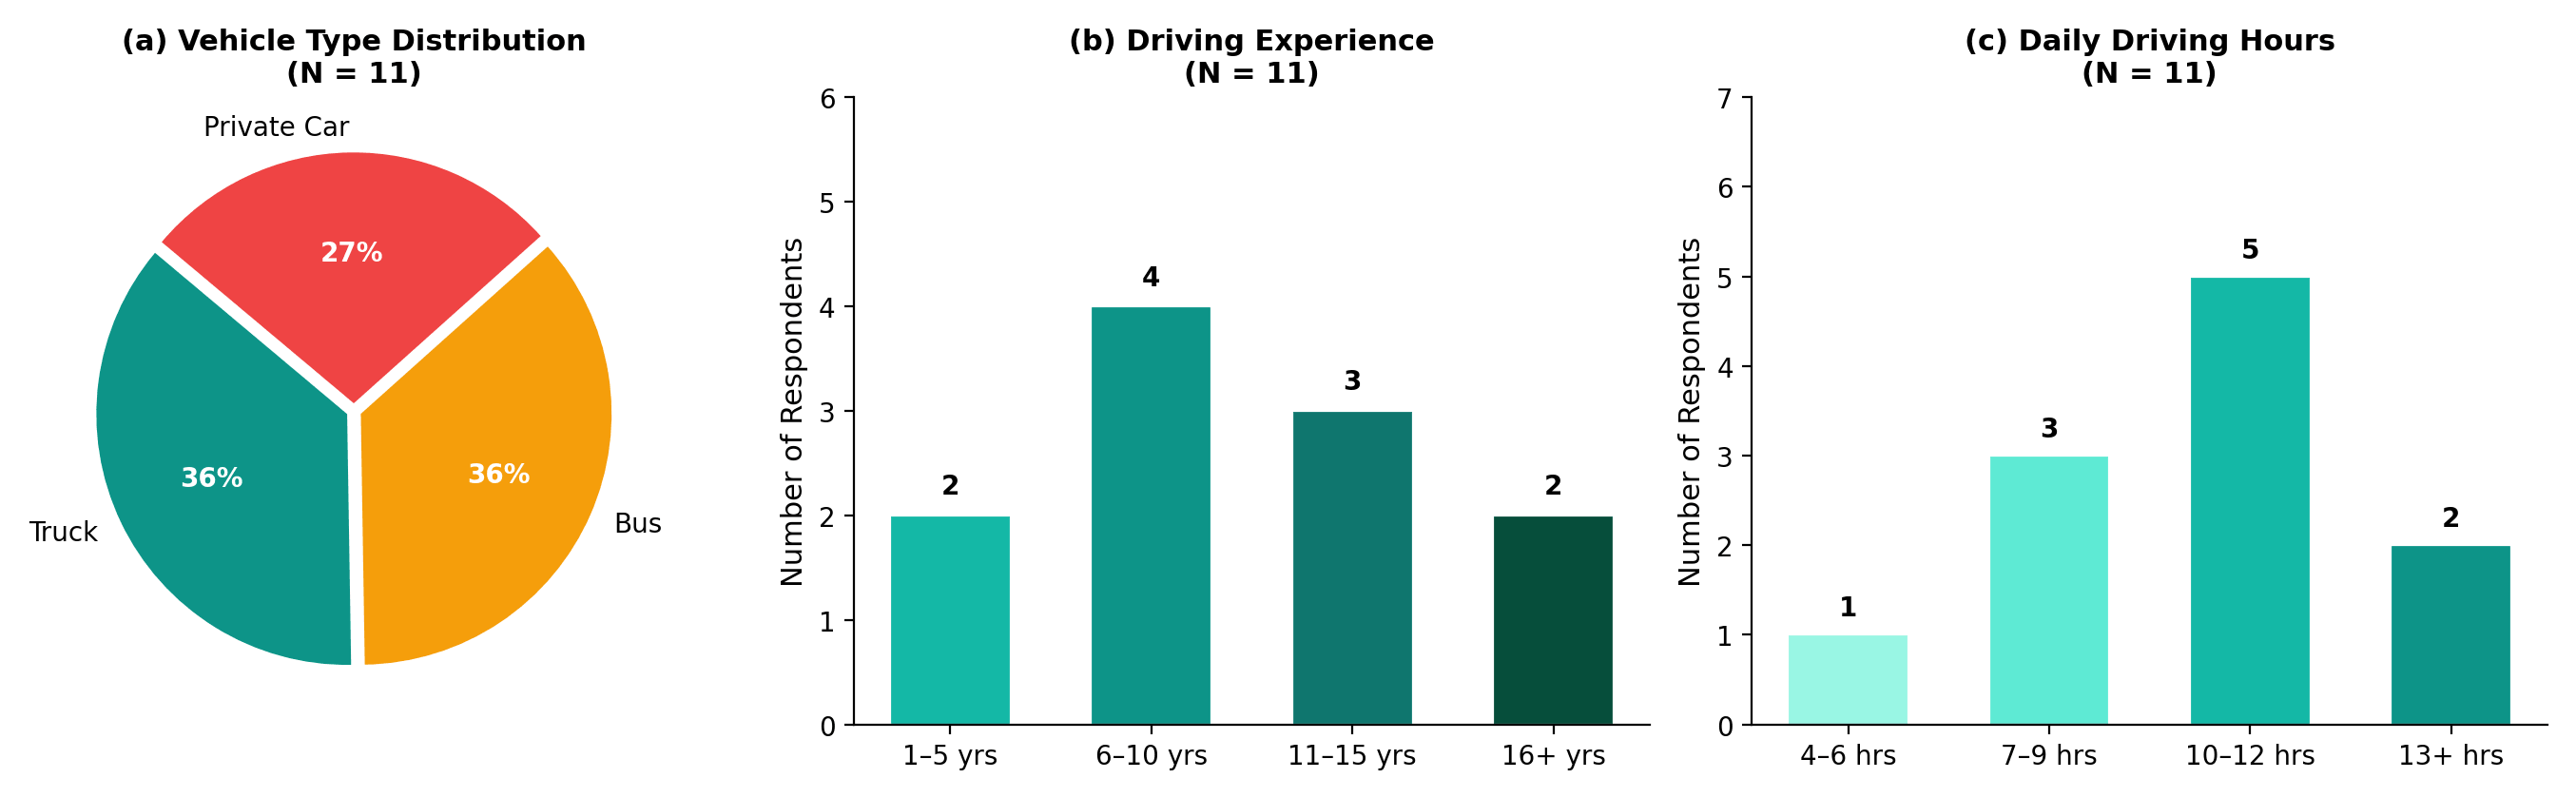
\includegraphics[width=\linewidth]{figures/fig_demographics.png}
\caption{Respondent demographics: (a)~Vehicle type distribution across the three target user groups, (b)~Driving experience showing majority in the 6--15 year range, and (c)~Daily driving hours confirming extended driving duration among the sample population (N~=~11).}
\label{fig:demographics}
\end{figure}

\subsection{Drowsiness Experience and Coping Strategies}

A majority of respondents (82\%, $n$~=~9) reported experiencing drowsiness at least once per week during driving. Critically, 73\% ($n$~=~8) reported having experienced at least one drowsiness-related safety incident (near-miss or close call), underscoring the urgency of effective monitoring systems. Peak drowsiness was most commonly reported between 12--3~AM, aligning with circadian low points and confirming the relevance of night-driving scenarios in the prototype design.

\begin{figure}[H]
\centering
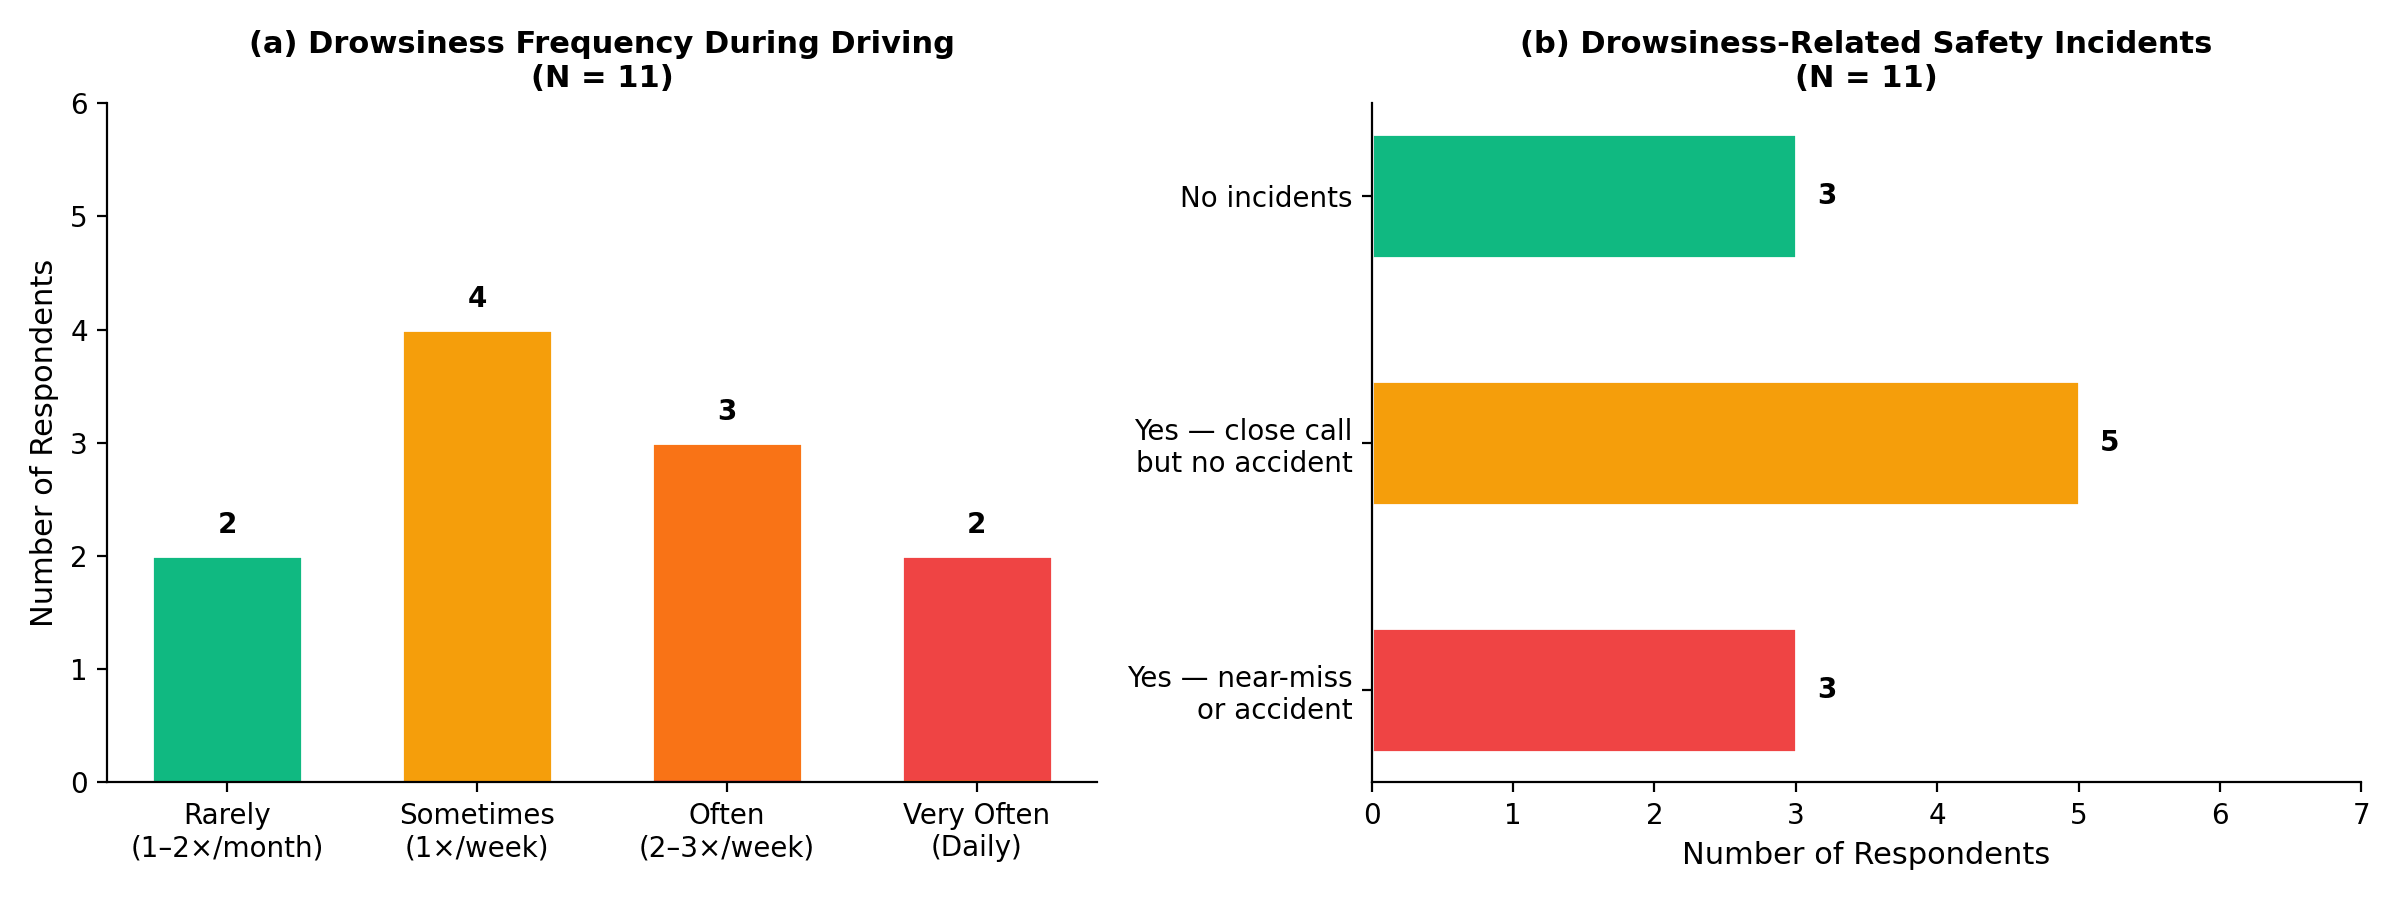
\includegraphics[width=\linewidth]{figures/fig_drowsiness_experience.png}
\caption{Drowsiness experience: (a)~Frequency of drowsiness during driving, with 82\% reporting weekly or more frequent episodes, and (b)~Drowsiness-related safety incidents, with 73\% having experienced at least one near-miss or close call (N~=~11).}
\label{fig:drowsiness_exp}
\end{figure}

Current coping strategies are predominantly informal and non-technological. Opening windows (82\%), splashing water on the face (64\%), and chewing betel leaf (55\%) were the most common approaches. Notably, only 36\% reported stopping to rest, suggesting a cultural and professional pressure to continue driving despite fatigue. These findings informed the design decision to position the system as a supportive companion (Saathi) rather than a directive controller, respecting existing coping practices while offering additional AI-based support.

\begin{figure}[H]
\centering
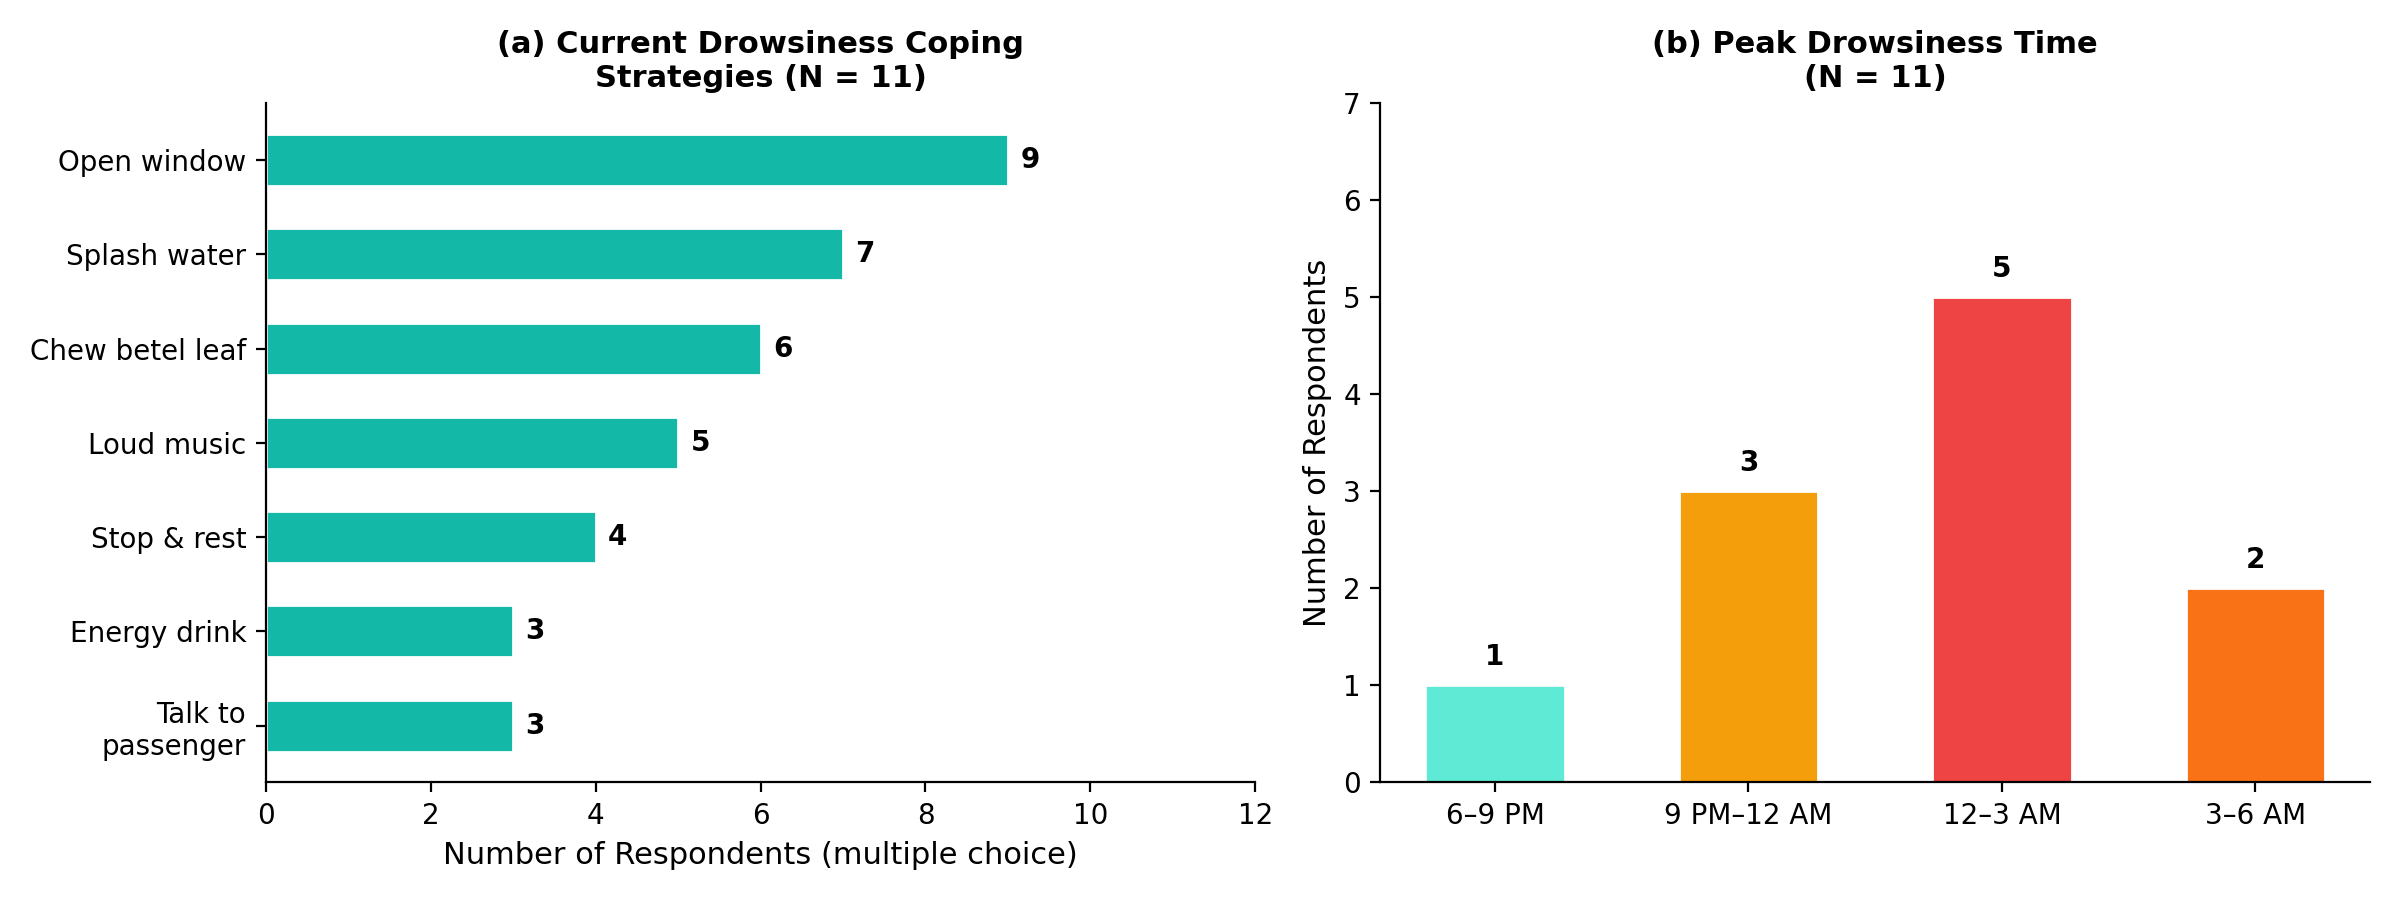
\includegraphics[width=\linewidth]{figures/fig_coping_times.png}
\caption{(a)~Current drowsiness coping strategies used by respondents (multiple choice), showing reliance on informal, non-technological approaches. (b)~Self-reported peak drowsiness times, with the highest frequency between 12--3~AM (N~=~11).}
\label{fig:coping}
\end{figure}

\subsection{Technology Attitudes and DMS Experience}

A critical finding was that \textbf{all 11 respondents (100\%) had zero prior experience with any driver monitoring system}. None had used, seen, or been exposed to commercial DMS solutions such as Mobileye, Tesla Autopilot monitoring, or Bosch DMS. This finding has significant design implications: the prototype must build trust from scratch, without the benefit of positive prior experience. It also validates the need for a progressive onboarding flow that introduces the concept of AI-based monitoring gradually.

\begin{figure}[H]
\centering
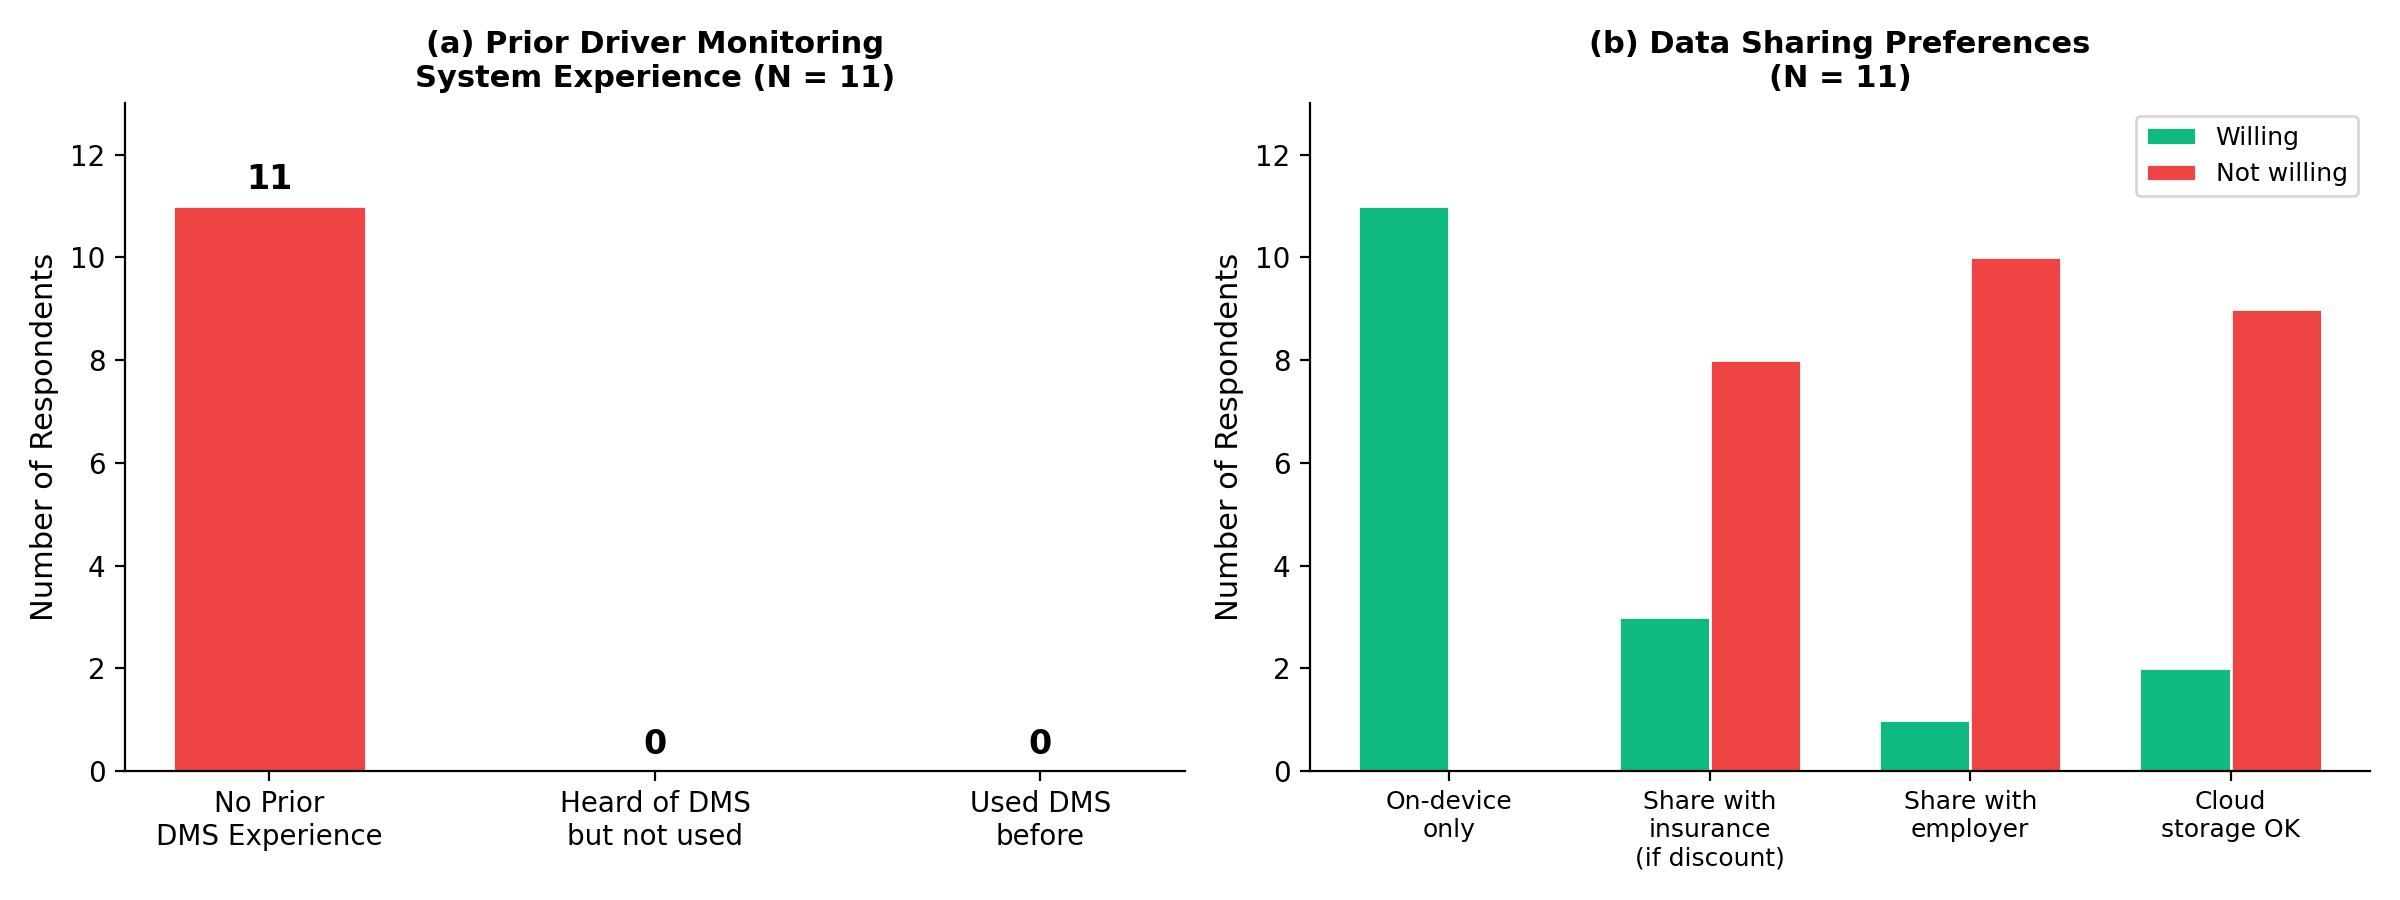
\includegraphics[width=\linewidth]{figures/fig_privacy_dms.png}
\caption{(a)~Prior DMS experience: all 11 respondents had no previous exposure to driver monitoring systems. (b)~Data sharing preferences: universal preference for on-device processing; strong resistance to employer data sharing (N~=~11).}
\label{fig:dms_privacy}
\end{figure}

Privacy concerns were pronounced among the primary stakeholders. All 11 drivers (100\%) preferred on-device data processing. When asked about hypothetical data sharing scenarios, only 3 drivers (27\%) were willing to share data with insurance companies (and only if offered a premium discount), and only 1 driver (9\%) was willing to share with their employer. These responses from the drivers themselves---not from the companies or insurers---directly informed the privacy-first design: on-device processing badges on every screen, all sharing toggles defaulting to OFF, and employer sharing locked behind an explicit warning. The system places data control entirely in the hands of the primary stakeholder (the driver).

\subsection{Feature Prioritization}

Respondents ranked 8 candidate features on a 1--5 Likert scale. The results (Figure~\ref{fig:feature_rank}) reveal a clear hierarchy:

\begin{figure}[H]
\centering
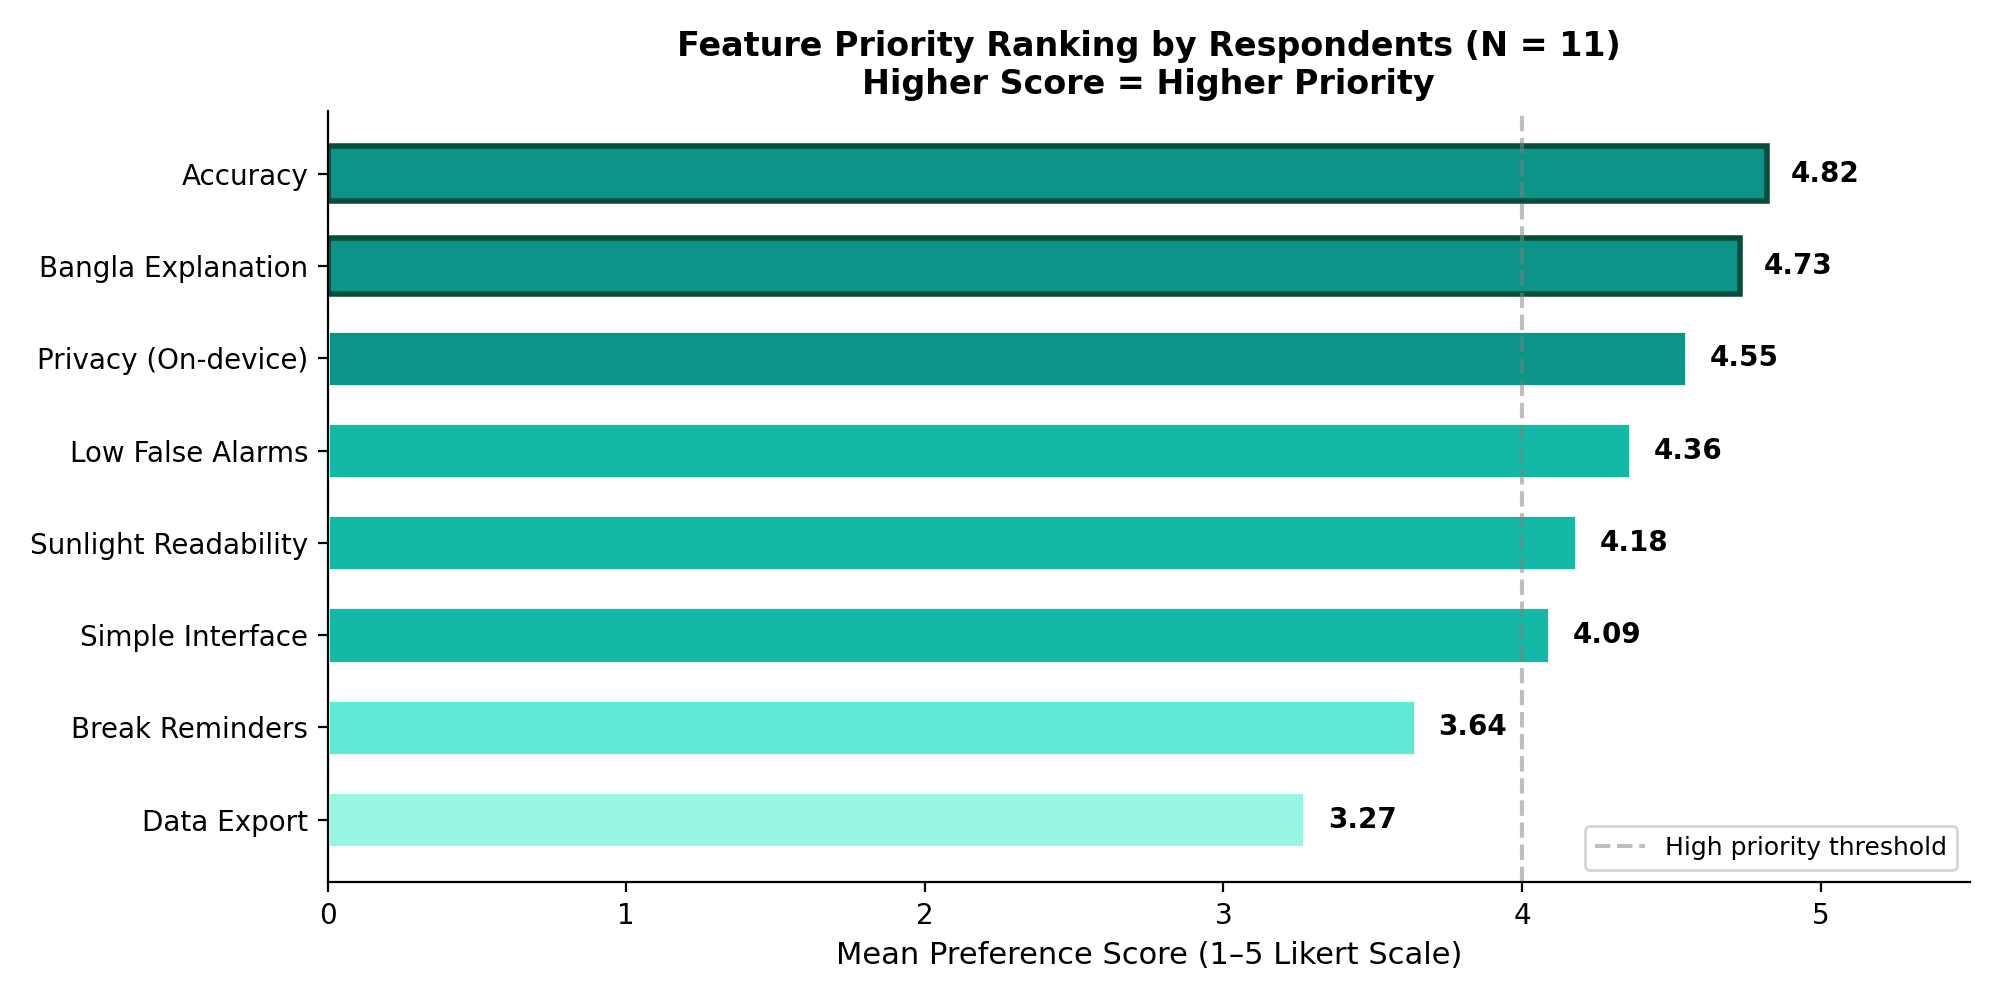
\includegraphics[width=\linewidth]{figures/fig_feature_ranking.png}
\caption{Feature priority ranking by respondents on a 1--5 Likert scale. Accuracy and Bangla plain-language explanation emerged as the two highest-priority features, both scoring above 4.7. The dashed line indicates the high-priority threshold (N~=~11).}
\label{fig:feature_rank}
\end{figure}

\textbf{Accuracy} (mean 4.82/5) and \textbf{Bangla plain-language explanation} (mean 4.73/5) were the two highest-ranked features, both significantly above the high-priority threshold of 4.0. This finding is the single most important design driver: the system must prioritize detection accuracy and must communicate in simple Bangla. Privacy (4.55) and low false alarm rate (4.36) followed closely. These four features collectively define the non-negotiable requirements for all three design variants.

\subsection{Alert and Interface Preferences}

Regarding alert modality, 64\% ($n$~=~7) preferred combined visual and audio alerts, while 27\% ($n$~=~3) preferred visual with vibration. Only 1 respondent preferred visual-only alerts. This guided the multi-modal alert design across all three prototypes.

\begin{figure}[H]
\centering
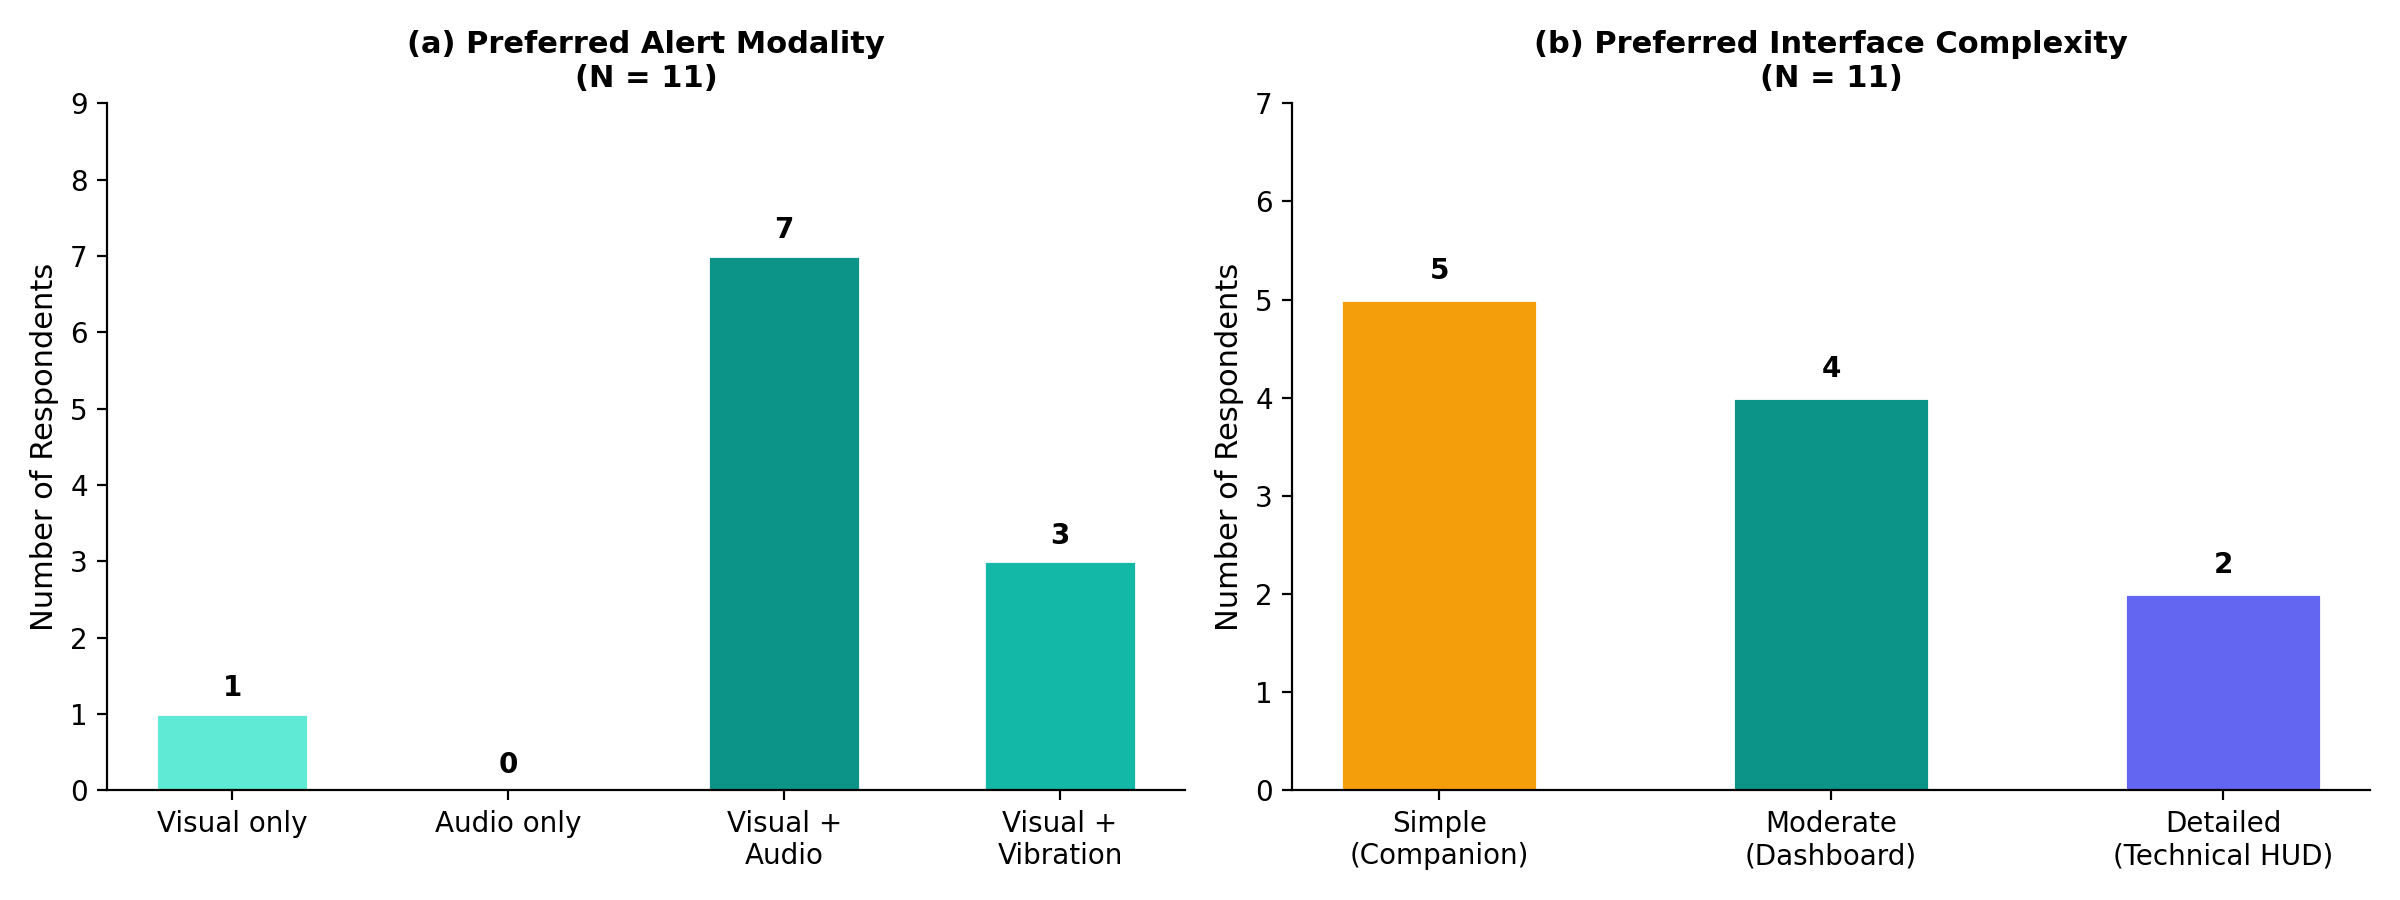
\includegraphics[width=\linewidth]{figures/fig_alert_interface.png}
\caption{(a)~Preferred alert modality: majority favor combined visual + audio alerts. (b)~Interface complexity preference: respondents split across simple, moderate, and detailed interfaces, validating the three-variant design approach (N~=~11).}
\label{fig:alert_interface}
\end{figure}

The interface complexity preference (Figure~\ref{fig:alert_interface}b) was the finding that most directly motivated the three-variant design approach. Respondents split across three clusters: 45\% ($n$~=~5) preferred a simple, companion-like interface, 36\% ($n$~=~4) preferred a moderate dashboard, and 18\% ($n$~=~2) preferred a detailed technical display. Because no single complexity level commanded a majority, a single-design approach would have left a significant portion of users underserved. This validated the persona-driven multi-variant strategy.

\subsection{Summary of Key Findings}

Table~\ref{tab:survey_summary} summarizes the five key findings and their direct impact on the prototype design decisions.

\begin{table}[H]
\centering
\caption{Key Survey Findings and Design Impact}
\label{tab:survey_summary}
\small
\begin{tabular}{|p{0.5cm}|p{3.2cm}|p{3.8cm}|}
\hline
\textbf{\#} & \textbf{Finding} & \textbf{Design Decision} \\
\hline
1 & Accuracy ranked \#1 by all respondents & Composite fatigue scoring with multiple indicators; personal calibration \\
\hline
2 & Bangla explanation highest preference (4.73/5) & Mandatory Bangla alert in all modes; English as subtitle only \\
\hline
3 & 0\% prior DMS experience & Progressive onboarding; Saathi character for trust building \\
\hline
4 & 100\% prefer on-device processing & Privacy badge on every screen; sharing defaults OFF; deletion default ON \\
\hline
5 & Interface preference split 45/36/18\% & Three design variants: Companion / Dashboard / HUD \\
\hline
\end{tabular}
\end{table}




\section{Prototype Design Methodology}

\subsection{Prototyping Approach}
The prototype was developed following a structured, iterative design process grounded in user-centered design principles. The approach consisted of four main phases: user research and data collection, persona-driven variant design, formative evaluation, and design unification.

\paragraph{Phase 1: User Research and Data Collection}
The design process began with a comprehensive survey administered to 11 Bangladeshi professional drivers---the primary stakeholders---including truck drivers, intercity bus operators, and private car drivers. The survey targeted exclusively the end-users of the proposed system, as they are the individuals who would directly interact with the drowsiness detection interface in safety-critical driving contexts. The survey instrument contained 60 questions organized across 8 thematic blocks covering demographic profile, drowsiness experience, coping strategies, technology attitudes, alert preferences, privacy concerns, language preferences, and feature prioritization. Responses were analyzed using Python-based tools including pandas for data processing, matplotlib and seaborn for visualization, and scipy for statistical analysis. The analysis was conducted in a Google Colab notebook designed to auto-scale as additional respondents are added.

Key findings that directly shaped the prototype design include: (1)~accuracy was ranked as the most important feature by all 11 respondents, (2)~Bangla plain-language explanation received the highest mean preference score among all feature items, (3)~no respondents had prior experience with any driver monitoring system, (4)~privacy was a significant concern with strong preference for on-device processing, and (5)~drivers expressed preferences ranging from minimal friendly interfaces to detailed technical dashboards, suggesting no single design would satisfy all users.

\paragraph{Phase 2: Persona-Driven Variant Design}
Based on the survey analysis, three distinct user personas were identified, each reflecting a different segment of the target driver population. Rather than producing a single interface, three separate prototype variants were developed, each tailored to the needs, technology comfort level, and interaction preferences of a specific persona. This approach ensured that diverse user expectations were explicitly addressed rather than averaged into a single compromise solution. Separate Lovable AI build prompts were crafted for each variant, treating the prompts as formal engineering artifacts with precise specifications for layout, typography, color systems, interaction patterns, state management, and bilingual content.

\paragraph{Phase 3: Formative Evaluation}
The three prototype variants were evaluated against the requirements identified during the formative analysis to assess how each design addressed functional, non-functional, and HCAI requirements. A requirements traceability analysis was conducted to map each system requirement to specific design features across all three variants. This evaluation also identified features that appeared in only one or two variants but were considered essential for the final system.

\paragraph{Phase 4: Design Unification}
Based on the evaluation results, the three variants were merged into a single unified prototype that incorporates a mode-switching architecture. Rather than forcing all users into one interface paradigm, the unified design allows drivers to select their preferred interaction mode during onboarding and switch modes at any time during use. This approach preserves the strengths of each persona-driven variant while providing a cohesive user experience under a single application framework. Prototyping allows designers to explore design alternatives and refine interaction strategies before full implementation \cite{ref12, ref13}.

\subsection{Tools and Technologies}

The prototype was constructed using a combination of user research tools, AI-assisted design platforms, and modern web development technologies.

\paragraph{Survey and Analysis Tools}
The user survey was administered in both Bangla and English. Data analysis was performed in Google Colab using Python libraries: pandas for data manipulation, matplotlib and seaborn for generating publication-quality figures, and scipy for statistical computations. The Colab notebook was designed with modular cells to allow re-execution as new survey data is collected.

\paragraph{Prototype Construction}
The functional prototype was built using Lovable AI, an AI-assisted web application builder. A comprehensive build prompt was engineered as a markdown document specifying every screen, component, state transition, animation, and content string. The technology stack specified in the prompt includes React with TypeScript for component architecture, Tailwind CSS for styling, Framer Motion for animations and transitions, Recharts for data visualizations, and Zustand for global state management.

\paragraph{Design References}
The interface design was informed by screenshots and descriptions of existing commercial driver monitoring systems---including Mobileye~8, Tesla Autopilot's driver monitoring interface, and Bosch DMS---which were shown to the primary stakeholders (drivers) during the survey as visual benchmarks. Drivers were asked to compare and evaluate features from these existing solutions, and their feedback (from the driver's perspective, not the manufacturer's) informed the prototype design decisions.

\subsection{AI Behavior Simulation}

Since the prototype is designed for demonstration and evaluation rather than real-time deployment with an actual AI model, AI functionality is simulated within the prototype environment using a deterministic simulation engine.

The simulation engine is implemented as a shared React hook (\texttt{useDrowsinessSimulation}) that runs across all three interface modes. It operates on a one-second timer cycle and simulates the following behaviors:

\begin{itemize}
    \item \textbf{PERCLOS Score Progression:} The Percentage of Eye Closure score gradually increases from a baseline of approximately 5\% to random peak values, simulating drowsiness onset over time.
    \item \textbf{Eye Aspect Ratio (EAR) Fluctuation:} The EAR value fluctuates realistically, decreasing as simulated drowsiness increases.
    \item \textbf{Blink Rate Variation:} Normal blink rate is simulated at 15--20 blinks per minute, decreasing to 5--10 blinks per minute during simulated drowsy states.
    \item \textbf{Head Pose Drift:} Subtle random variations in pitch, yaw, and roll simulate head nodding and tilting behaviors associated with fatigue.
    \item \textbf{Event Triggering:} Every 45--90 seconds, the engine triggers a drowsiness event with randomized severity (Level~1: Caution, Level~2: Warning, Level~3: Danger), generating alert cards with Bangla plain-language explanations and English technical descriptions.
    \item \textbf{AI Confidence Display:} Confidence values are displayed in the 85--98\% range, simulating the model's certainty about its detection.
\end{itemize}

This simulation approach allows evaluators and users to experience the full interaction flow—including alert generation, dismissal, false alarm flagging, and historical data review—without requiring a live camera feed or trained AI model.


\section{Prototype Artifacts and Interface Design}

Three functional prototype variants were designed and built using Lovable AI, each targeting a specific driver persona identified from the survey data. Each prototype was generated from a carefully engineered build prompt that serves as a formal design specification. This section presents the personas, the complete prompts used to generate each design (reproduced verbatim), the deployed prototype interfaces, and the interaction scenarios used for evaluation.

\subsection{Persona-to-Design Mapping}

Table~\ref{tab:persona_design} summarizes how each persona maps to a design variant. The three personas were derived exclusively from the primary stakeholder survey data, with each persona representing a distinct cluster of preferences observed among the 11 professional drivers. The mapping is grounded in the survey finding that drivers expressed widely varying preferences for interface complexity---from ``I just want something simple'' (low-literacy truck drivers) to ``I want to see the data'' (tech-savvy private drivers)---motivating a multi-variant approach rather than a single averaged design.

\begin{table}[h]
\centering
\caption{Persona-to-Design Variant Mapping}
\label{tab:persona_design}
\small
\begin{tabular}{|p{1.4cm}|p{1.2cm}|p{1.6cm}|p{2.8cm}|}
\hline
\textbf{Persona} & \textbf{Tech Literacy} & \textbf{Design Variant} & \textbf{Core Design Principle} \\
\hline
Rahim (Truck Driver, 42) & Low & Design~2: Companion (Saathi) & Trust through emotional connection; no technical metrics \\
\hline
Karim (Bus Driver, 35) & Moderate & Design~1: Dashboard (DrowsyGuard) & Clarity through status-at-a-glance with bilingual alerts \\
\hline
Fatema (Private Driver, 28) & High & Design~3: HUD (DrowsyHUD) & Transparency through full real-time metric exposure \\
\hline
\end{tabular}
\end{table}

% ================================================================
% DESIGN 1: DROWSYGUARD (DASHBOARD MODE)
% ================================================================
\subsection{Design~1: DrowsyGuard --- Dashboard Mode}

\paragraph{Target Persona: Karim (Fleet Bus Operator)}
Karim is a 35-year-old intercity bus driver with moderate smartphone proficiency who manages a fixed route schedule for a transport company. He is accountable for passenger safety and wants clear, trustworthy status information without being overwhelmed by technical detail. The Dashboard Mode provides a professional, status-focused interface with bilingual alerts and confidence indicators that match his moderate technology comfort level.

\paragraph{Lovable AI Build Prompt (Verbatim)}
The following prompt was provided verbatim to Lovable AI to generate Design~1:

\begin{promptbox}[Prompt~1: DrowsyGuard --- Dashboard Mode for Bangladeshi Professional Drivers]
Build a mobile dashboard app called ``DrowsyGuard'' for Bangladeshi professional drivers. The app is a real-time AI drowsiness detection system. Use a dark teal (\#0D9488) and white color scheme. Primary language is Bangla (Bengali script) with English subtitles.

\textbf{MAIN SCREEN (Driving Mode):} Full-screen dark background (\#0F172A). Center: Large circular status indicator, 200px diameter. States: ``Monitoring'' (teal glow), ``Caution!'' (amber pulse), ``Danger!'' (red pulse). Top-left: Small green badge ``All data on your device'' with lock icon. Top-right: Trip timer and current sensitivity setting (Conservative / Balanced / Relaxed). Bottom: Three icon buttons: (1) Flashlight icon = false alarm flag, (2) Map pin = nearest rest stop, (3) Info = why was I alerted?

\textbf{ALERT CARD (slides up from bottom):} White card with coral (\#E8571A) top border 4px. Large icon: eye with drooping lid. Bangla text (24px bold): reason in plain language e.g.\ ``Your eyes are getting heavy.'' English subtitle (14px): ``Eyes closing detected --- 3 blinks in 4 seconds.'' Two buttons: ``I'm okay'' (dismisses) and ``Take rest'' (shows rest stops). Confidence bar at bottom: ``Confidence: 87\%'' with teal fill.

\textbf{REST STOP SCREEN:} Map view with 3 nearest stops pinned. Each stop card: Name, distance in km, estimated drive time, icons for toilet/food/fuel. ``Stop here'' button in coral.

\textbf{SETTINGS SCREEN:} Sensitivity: 3-button toggle (Conservative / Balanced / Relaxed). Privacy: Toggle for insurance sharing (default OFF), employer sharing (default OFF, locked with warning icon). Data: ``Delete data after trip'' toggle, default ON. About: Fairness certification card: ``Fitzpatrick Skin Tone Scale tested'' with checkmark. System: Off-switch with ``Auto-restarts in 30 seconds'' warning.

\textbf{WEEKLY SUMMARY SCREEN (PIN-protected):} Bar chart of drowsiness events by day. Top 3 highest-risk time slots. Personalized tip in Bangla based on patterns. Share button (disabled by default, shows consent dialog when tapped).

Design style: Clean, minimal, rounded corners (16px), no shadows, Noto Sans Bengali font, large tap targets (minimum 48px). Works in direct sunlight --- high contrast mode by default.
\end{promptbox}

\begin{figure*}[t]
\centering
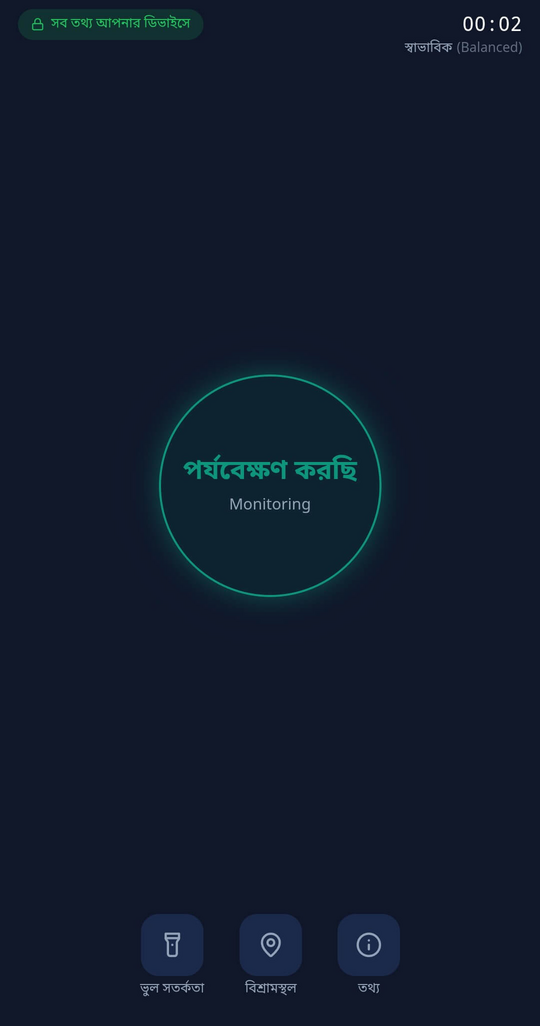
\includegraphics[height=5.5cm]{figures/DrowsyGuard-Monitoring.png}\hfill
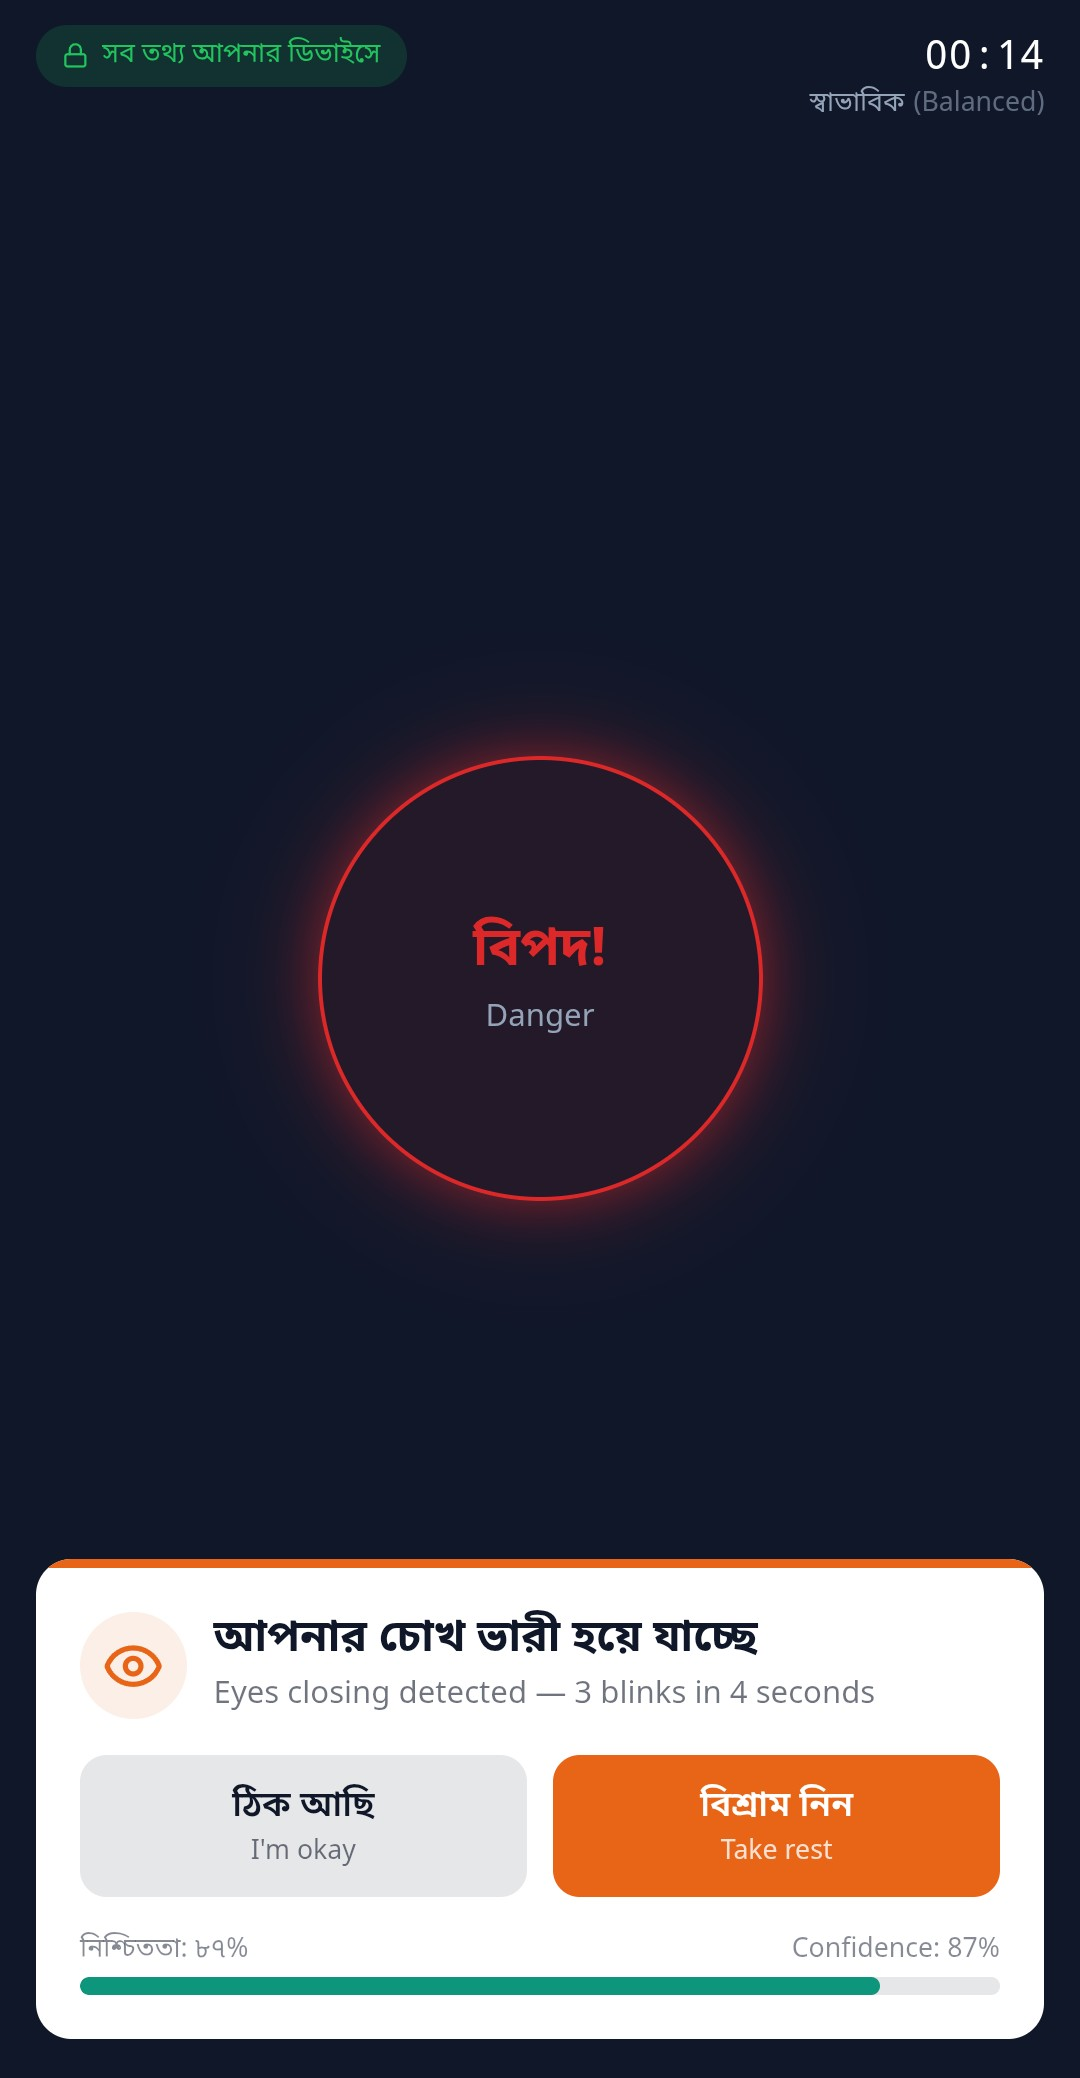
\includegraphics[height=5.5cm]{figures/DrowsyGuard-Alert.png}\hfill
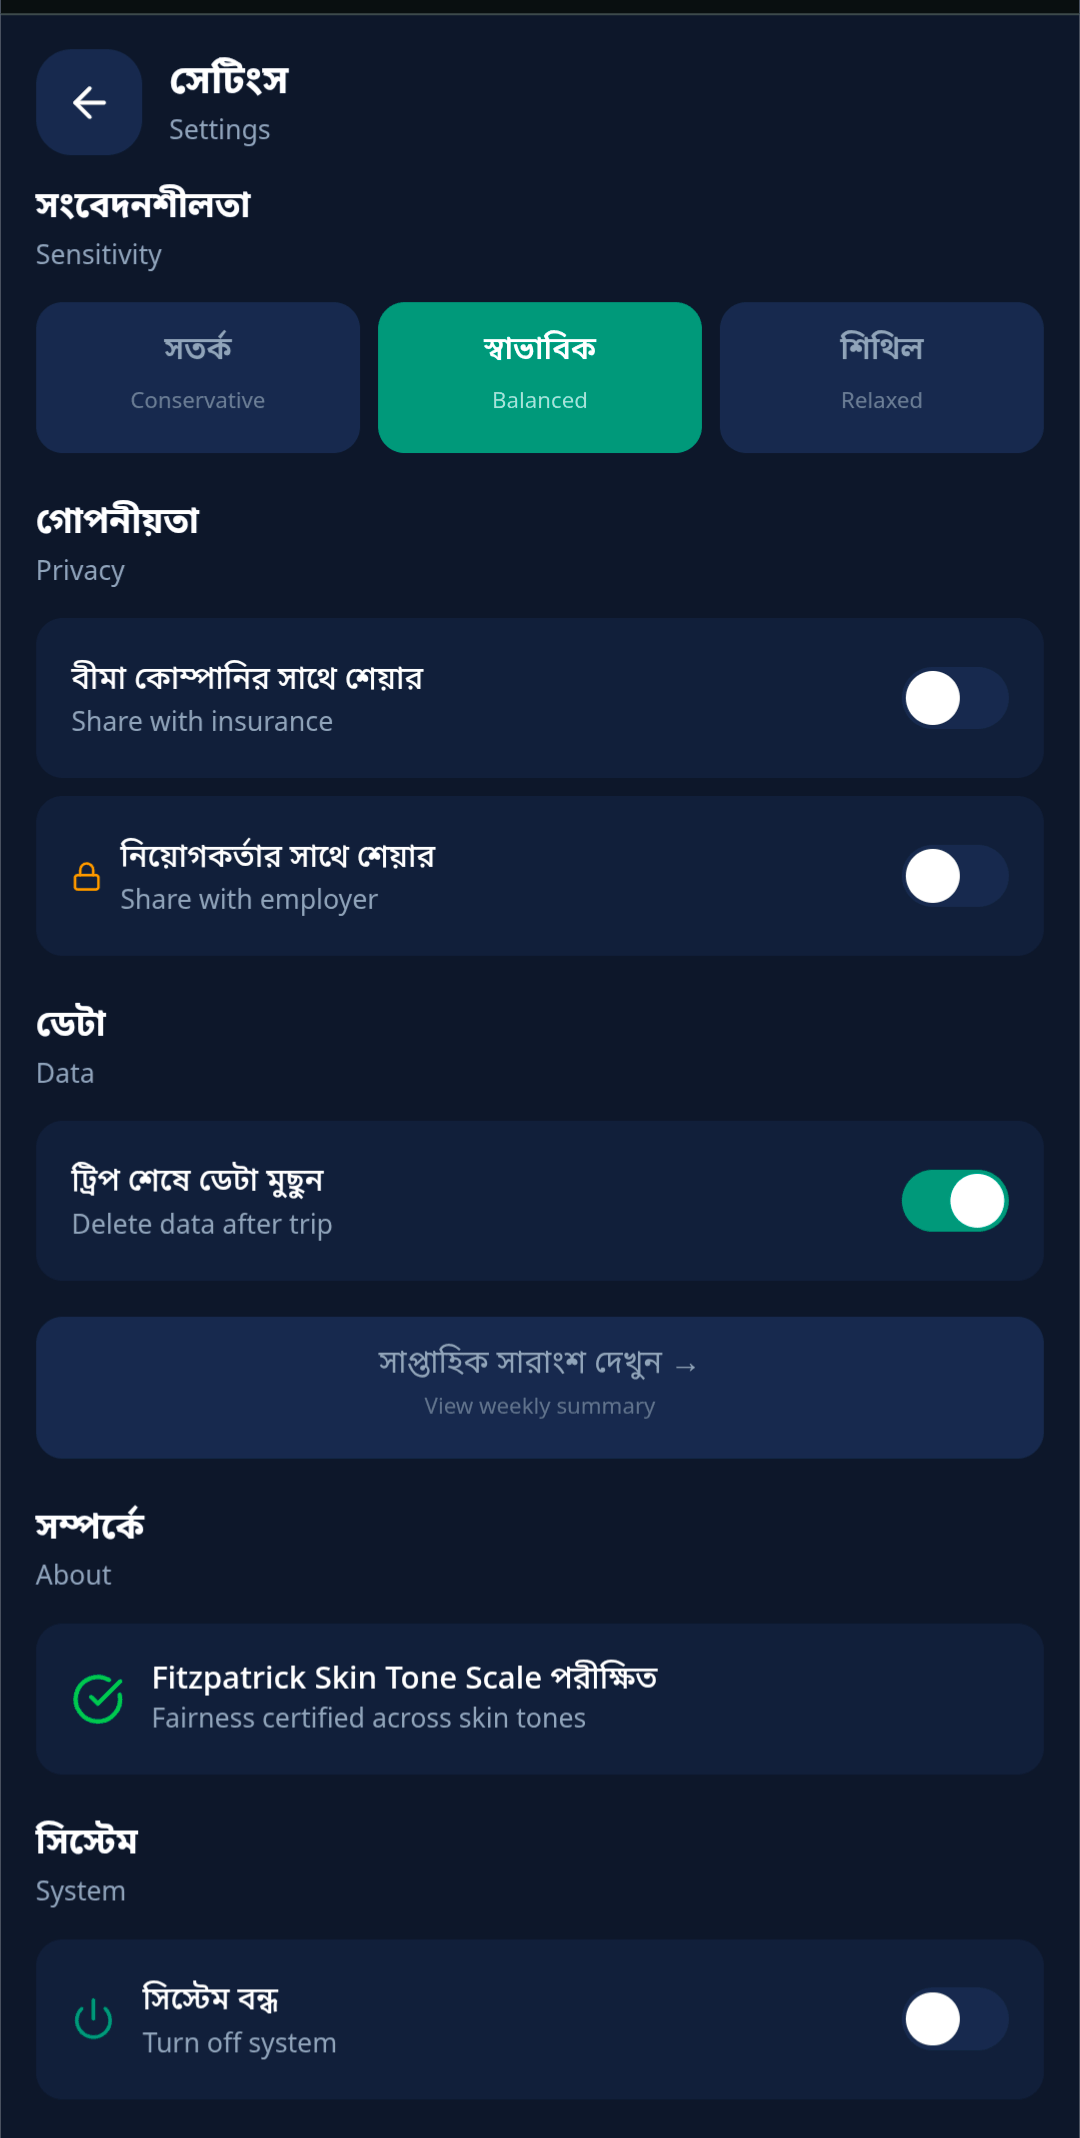
\includegraphics[height=5.5cm]{figures/DrowsyGuard-Settings.png}\hfill
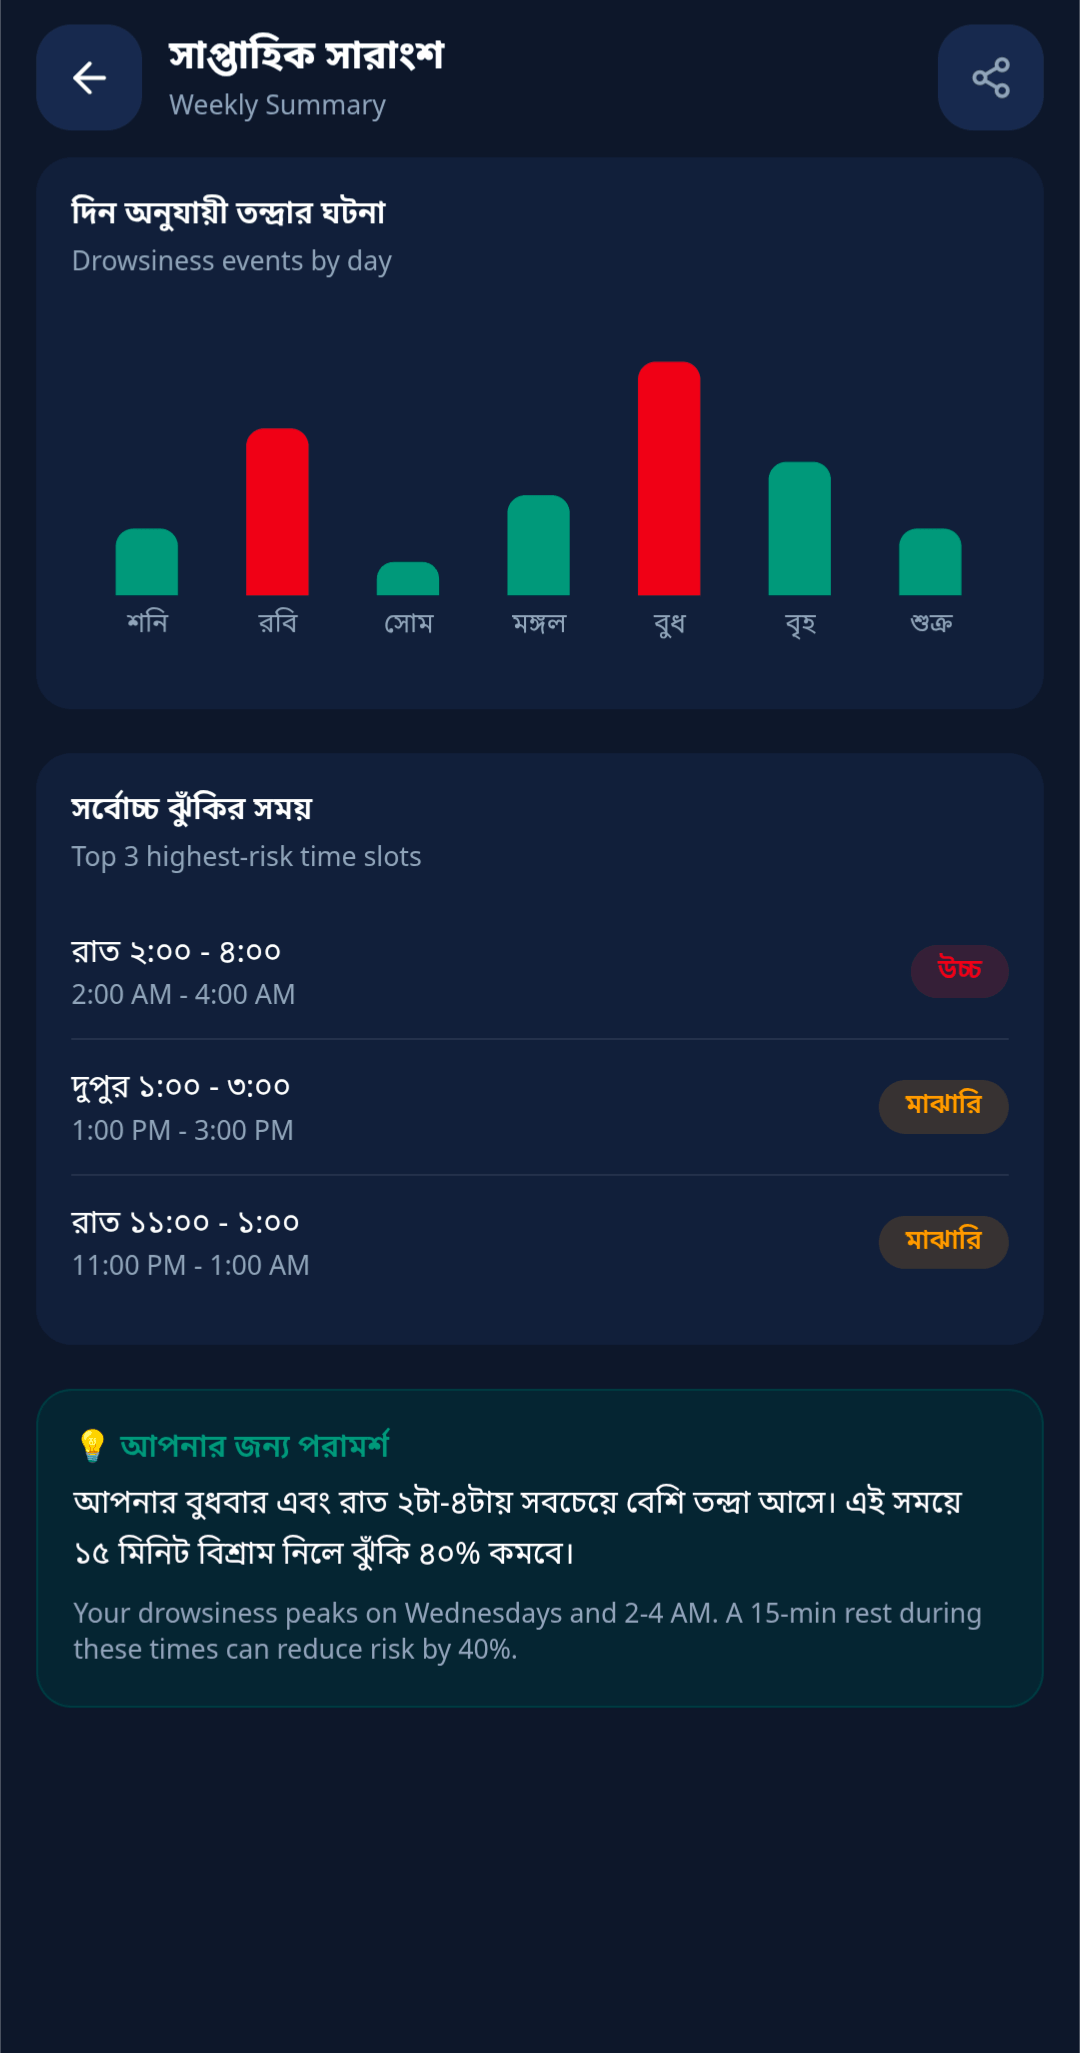
\includegraphics[height=5.5cm]{figures/DrowsyGuard-Stats.png}

\footnotesize\textbf{Source:} \url{https://drowsyguard-bangla-driver.lovable.app}
\caption{Design~1 --- DrowsyGuard (Dashboard Mode) targeting Persona~2 (Karim). The design uses a large circular status indicator for at-a-glance monitoring, bilingual alert cards with confidence percentage for trust calibration, and a privacy badge confirming on-device processing.}
\label{fig:design1}
\end{figure*}

\paragraph{HCAI Principle Implementation in Design~1}
Table~\ref{tab:hcai_d1} maps HCAI principles to specific features in the DrowsyGuard interface.

\begin{table}[h]
\centering
\caption{HCAI Principles in Design~1 (DrowsyGuard)}
\label{tab:hcai_d1}
\small
\begin{tabular}{|p{2cm}|p{5.5cm}|}
\hline
\textbf{Principle} & \textbf{Implementation} \\
\hline
Transparency & Circular indicator communicates state via color (teal/amber/red) and Bangla label \\
\hline
Explainability & Alert card: Bangla reason + English description + confidence \% \\
\hline
Reliability & Multiple indicators combined behind single status; composite scoring \\
\hline
Human Oversight & Dismiss alert, flag false alarm, navigate to rest stop (all single-tap) \\
\hline
\end{tabular}
\end{table}


% ================================================================
% DESIGN 2: SAATHI (COMPANION MODE)
% ================================================================
\subsection{Design~2: Saathi --- Companion Mode}

\paragraph{Target Persona: Rahim (Long-Haul Truck Driver)}
Rahim is a 42-year-old truck driver with limited formal education and minimal smartphone experience. He frequently experiences drowsiness on overnight routes but relies on informal coping strategies. He is skeptical of monitoring technology but values safety for his family. The Companion Mode replaces all technical metrics with an animated character (Saathi) that communicates through conversational Bangla, building trust through emotional connection rather than information density.

\paragraph{Lovable AI Build Prompt (Verbatim)}
The following prompt was provided verbatim to Lovable AI to generate Design~2:

\begin{promptbox}[Prompt~2: Saathi --- Companion Mode for Non-Tech-Savvy Bangladeshi Drivers]
Build a mobile companion app called ``Saathi'' (meaning ``Companion'') for Bangladeshi drivers who are not tech-savvy. The app monitors drowsiness using AI but presents itself as a friendly driving companion. Warm color scheme: off-white (\#FFFBF7) background, teal (\#0D9488) for the character, coral (\#E8571A) for alerts.

\textbf{CHARACTER DESIGN --- Saathi:} The main interface element is an animated character --- a large circular eye (150px diameter) that represents the AI companion. Emotional states: \textit{Alert/Happy}: Bright open eye, teal iris, gentle idle blink every 3--4s. \textit{Watching}: Slightly narrowed eye, amber iris, increased blink rate. \textit{Worried}: Drooping upper eyelid (half-closed), coral iris, soft pulse glow. \textit{Critical}: Heavy drooping lid, red iris, shaking/vibration animation, red pulse ring.

\textbf{MAIN SCREEN:} Warm white background (\#FFFBF7). Top bar: Tiny lock icon (teal) + trip timer. Center (60\% of screen): Saathi character with speech bubble. Bubbles rotate every 30s: Alert: ``You're doing great! Drive safe.'' Watching: ``Stay a bit careful.'' Worried: ``Brother, will you take some rest?'' Bottom: Single status text --- ``Safe'' / ``Stay alert'' / ``Take rest.'' Three icon buttons: False alarm flag, rest place finder, explanation.

\textbf{ALERT (Companion Style):} Saathi character becomes large and shakes gently. Speech bubble shows conversational Bangla: ``Brother, your eyes are getting heavy. Will you take some rest?'' Two large buttons: ``I'm okay'' with checkmark, ``Show rest places'' with map pin. NO technical metrics shown --- confidence is hidden.

\textbf{WEEKLY SUMMARY:} Saathi gives a weekly report as speech bubble. Smiley-face chart (5 smileys = great week, 1 = tough week). Top tip in conversational Bangla. Share button hidden by default.

\textbf{SETTINGS (``Saathi's Preferences''):} Saathi asks questions conversationally: ``Should I be quieter at night?'' Yes/No. ``Share data with insurance?'' Yes/No with explanation. Language toggle: Bangla / English.

Design: Noto Sans Bengali font, large text (minimum 18px body), rounded everything (24px radius), character animation using CSS or Lottie, warm and inviting --- not clinical or intimidating. Must feel like a helpful friend, not a surveillance device.
\end{promptbox}

% \noindent\textbf{Deployed Prototype URL:} \url{https://saathi-driver-friend.lovable.app}

\begin{figure*}[t]
\centering
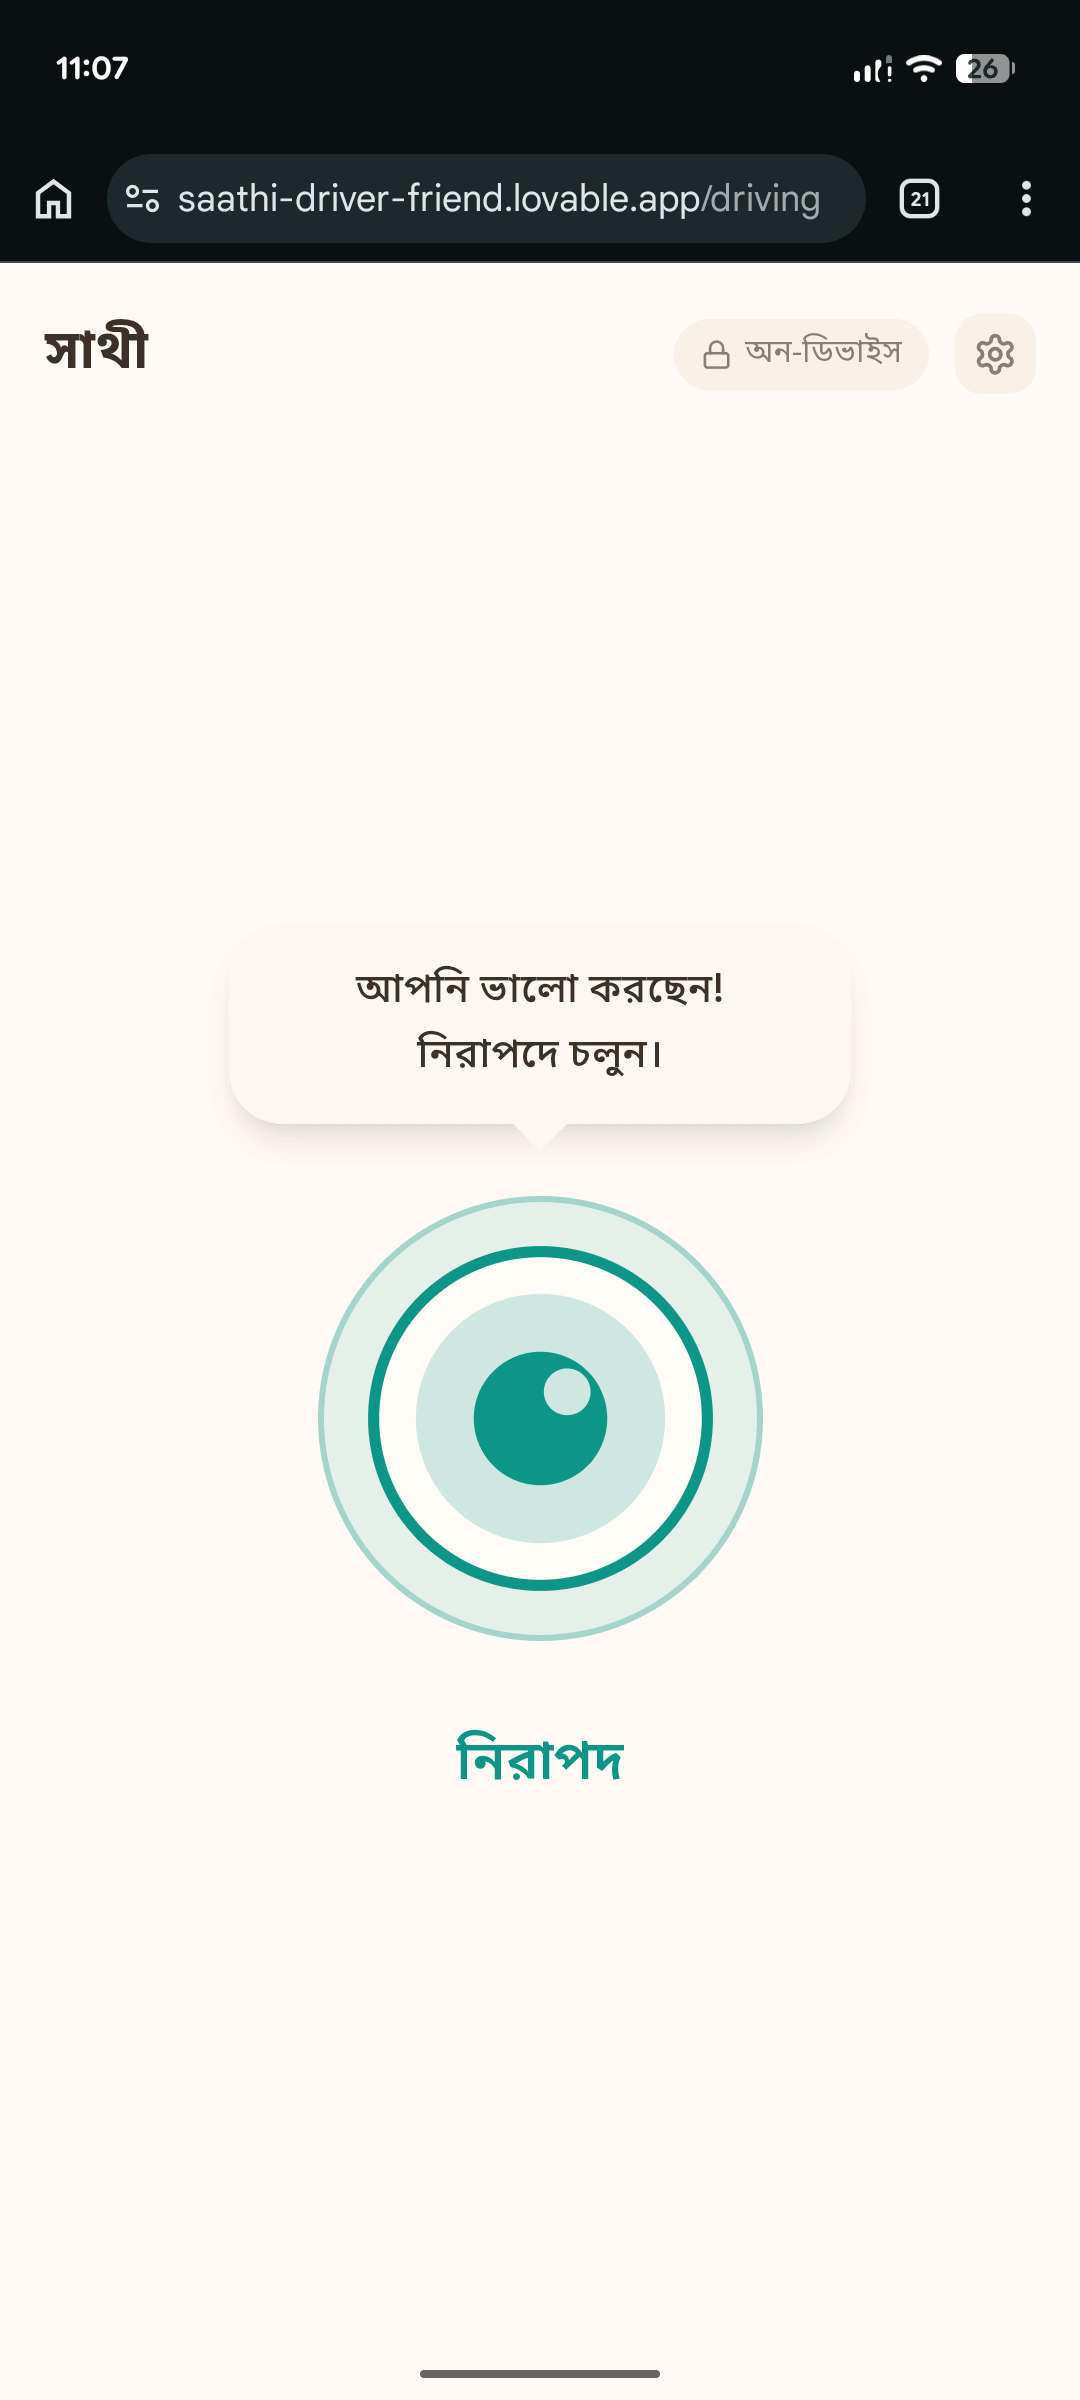
\includegraphics[height=5.5cm]{figures/Saathi-Monitoring.png}\hfill
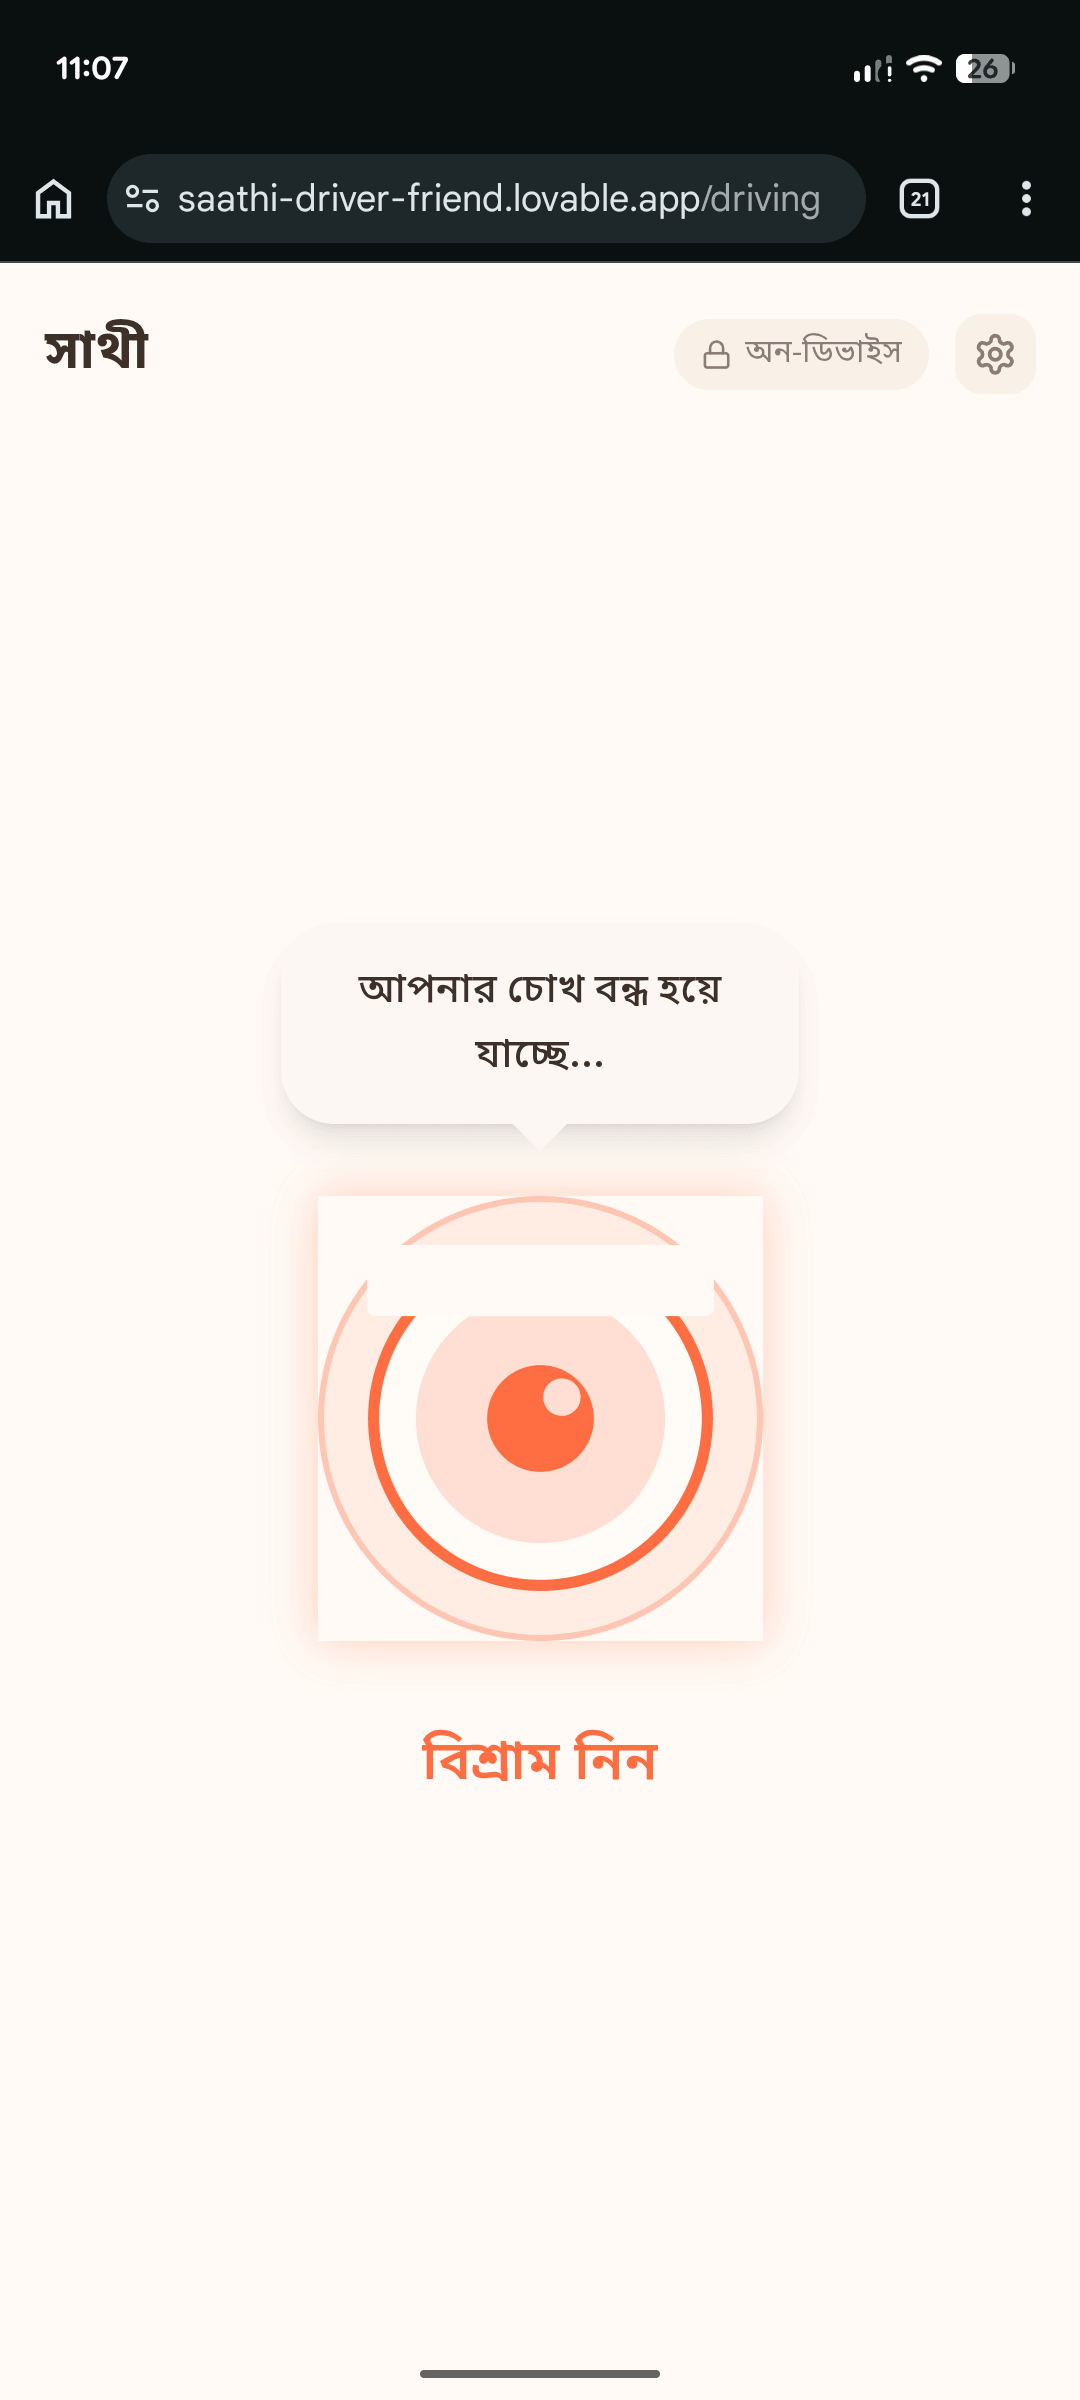
\includegraphics[height=5.5cm]{figures/Saathi-Explain.png}\hfill
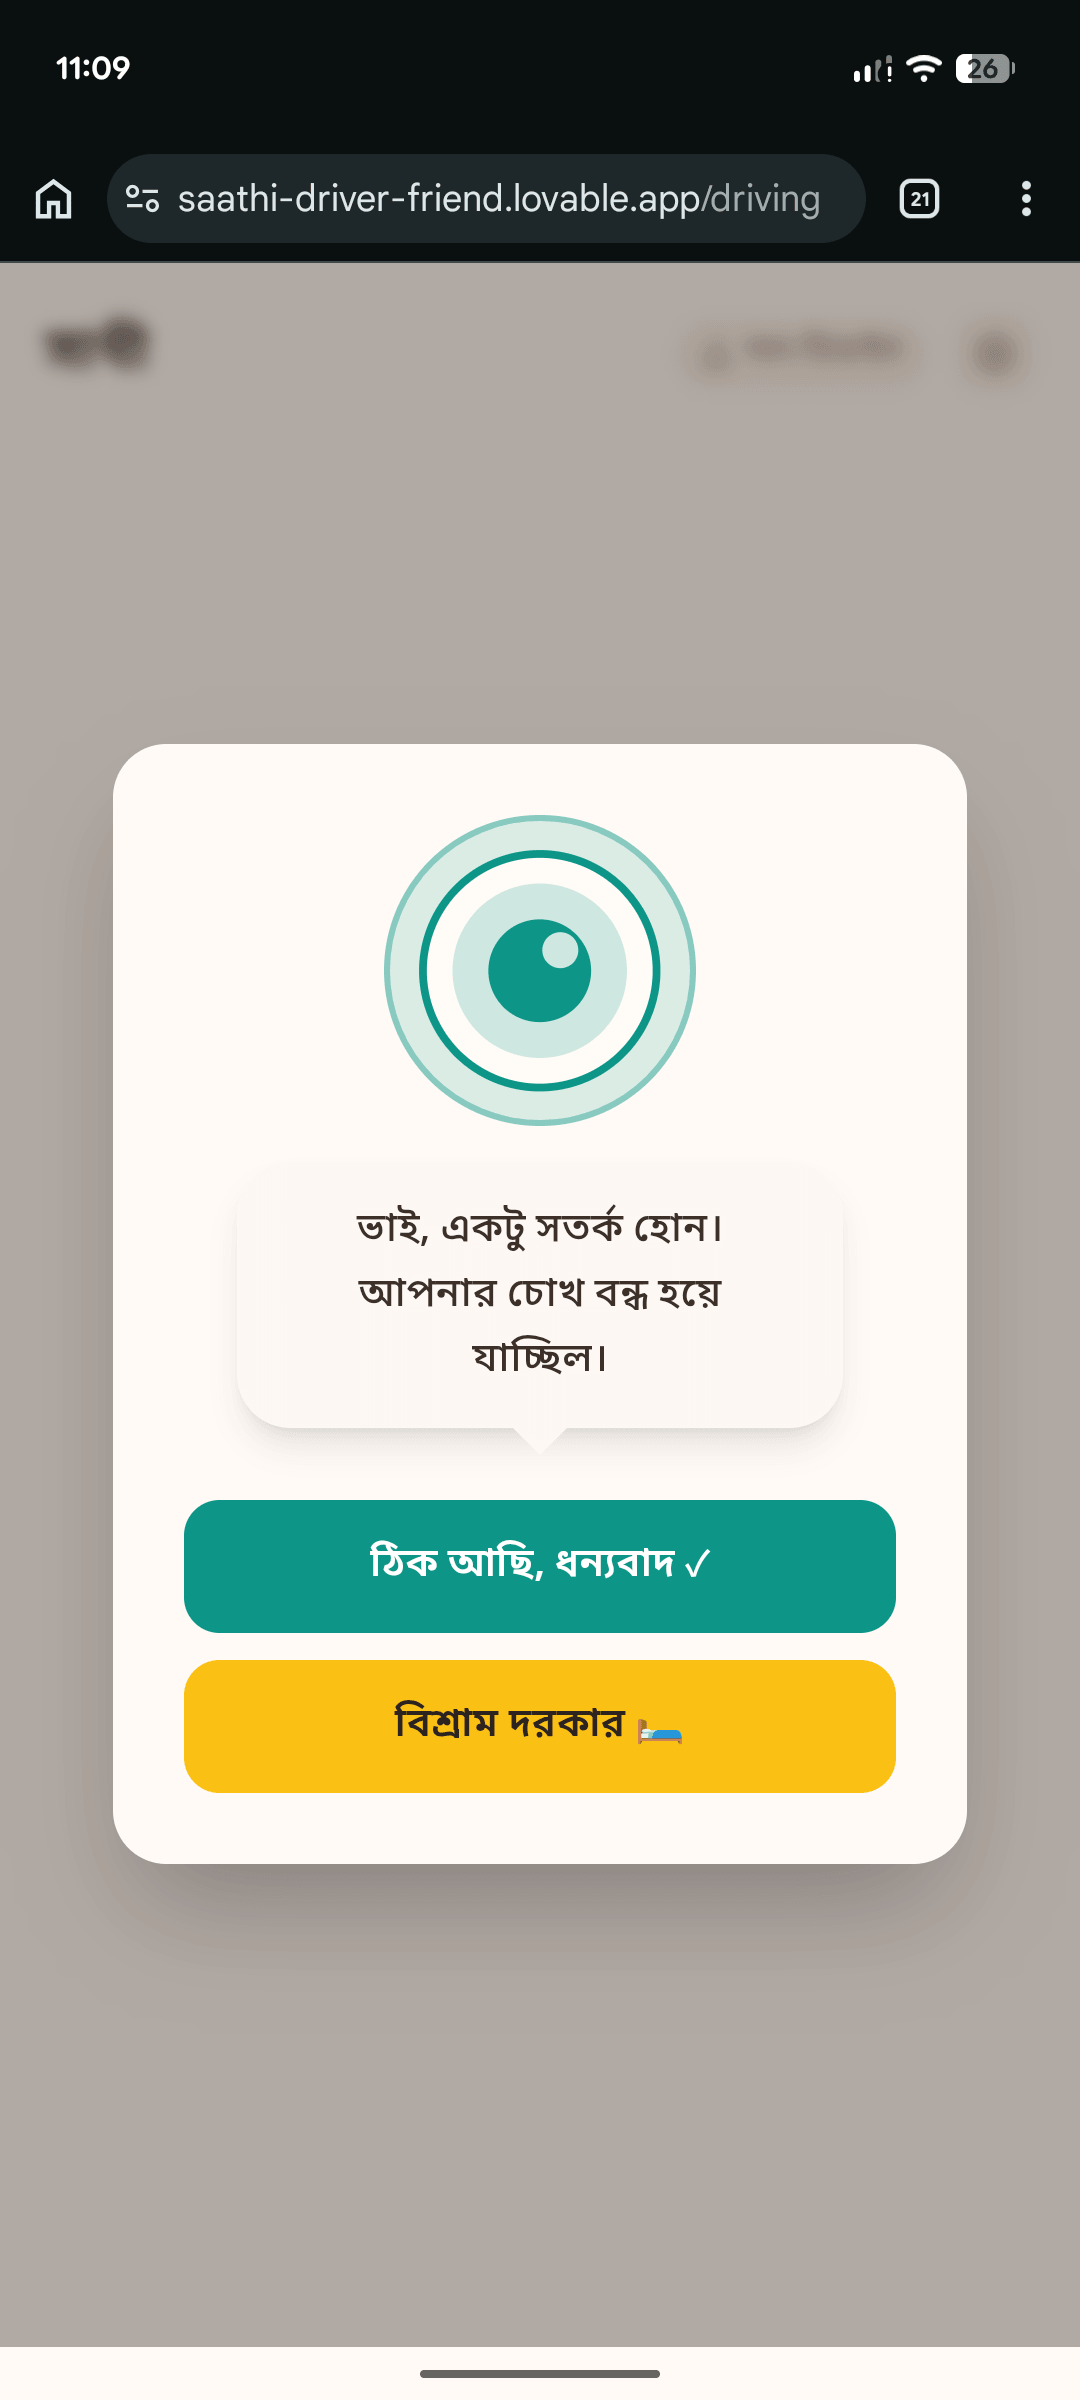
\includegraphics[height=5.5cm]{figures/Saathi-Warning.png}\hfill
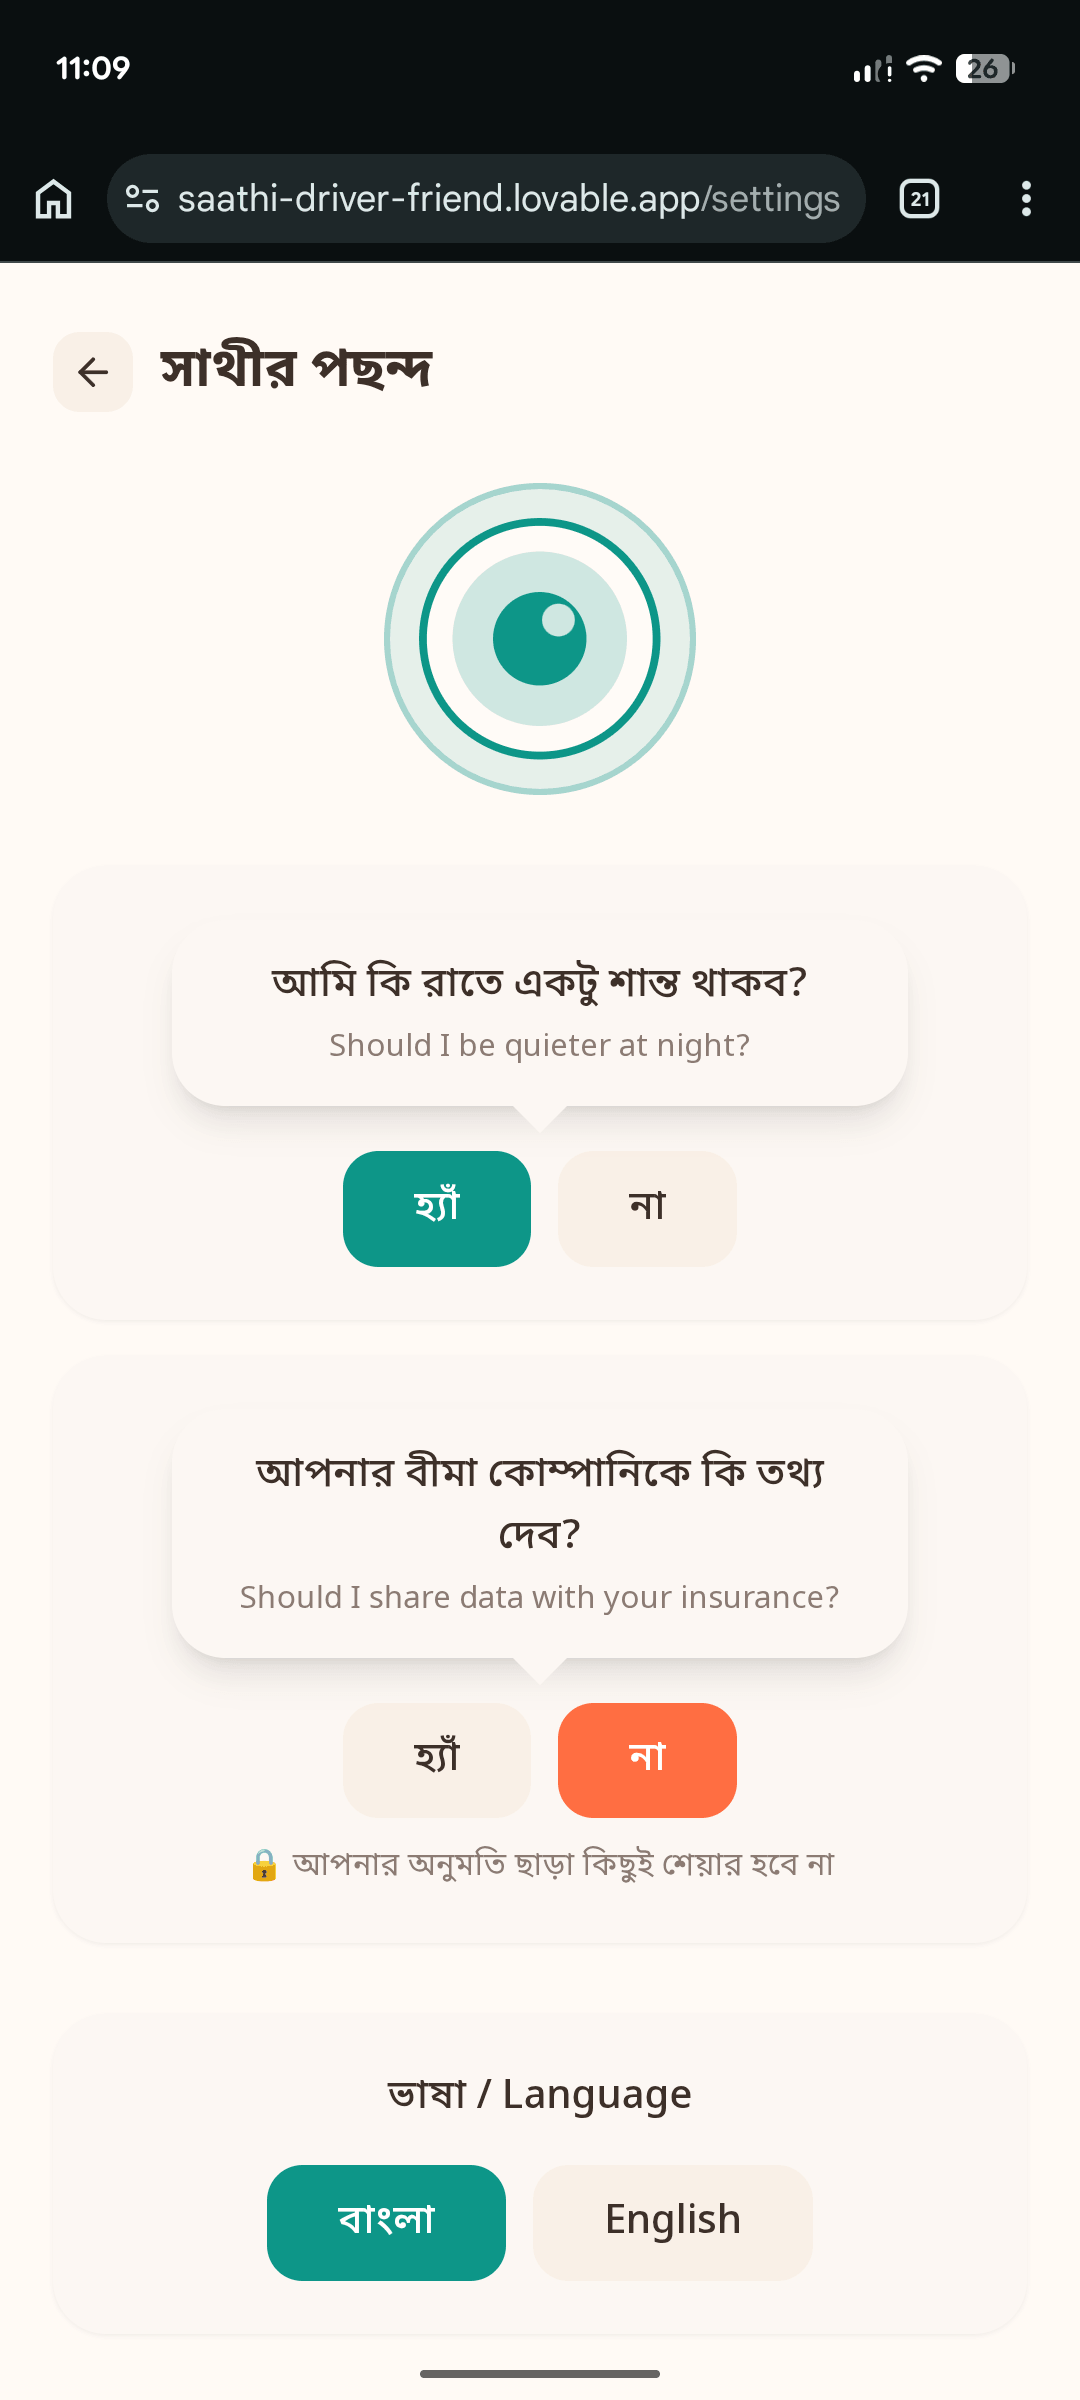
\includegraphics[height=5.5cm]{figures/Saathi-Settings.png}

\footnotesize\textbf{Source:} \url{https://saathi-driver-friend.lovable.app}
\caption{Design~2 --- Saathi (Companion Mode) targeting Persona~1 (Rahim). The interface centers on the animated Saathi character whose emotional state visually encodes drowsiness levels. All communication is in simple conversational Bangla with zero technical metrics. The warm color palette and rounded elements create a non-intimidating, friendly experience.}
\label{fig:design2}
\end{figure*}

\paragraph{HCAI Principle Implementation in Design~2}
Table~\ref{tab:hcai_d2} maps HCAI principles to specific features in the Saathi interface.

\begin{table}[h]
\centering
\caption{HCAI Principles in Design~2 (Saathi)}
\label{tab:hcai_d2}
\small
\begin{tabular}{|p{2cm}|p{5.5cm}|}
\hline
\textbf{Principle} & \textbf{Implementation} \\
\hline
Transparency & Saathi's eye expression and iris color directly encode monitoring state \\
\hline
Explainability & Conversational Bangla: ``Brother, your eyes are getting heavy'' (no jargon) \\
\hline
Reliability & Multiple indicators drive character state; complexity hidden from user \\
\hline
Human Oversight & Dismiss, flag false alarm, choose rest stop; system never acts autonomously \\
\hline
\end{tabular}
\end{table}

% ================================================================
% DESIGN 3: DROWSYHUD (TECHNICAL HUD MODE)
% ================================================================
\subsection{Design~3: DrowsyHUD --- Technical HUD Mode}

\paragraph{Target Persona: Fatema (Tech-Savvy Private Driver)}
Fatema is a 28-year-old university-educated private driver comfortable with data-rich applications. She wants to see exactly what the AI is detecting, how confident it is, and how her fatigue patterns evolve over time. The HUD Mode exposes all real-time detection metrics in an instrument-panel layout, providing maximum technical transparency.

\paragraph{Lovable AI Build Prompt (Verbatim)}
The following prompt was provided verbatim to Lovable AI to generate Design~3:

\begin{promptbox}[Prompt~3: DrowsyHUD --- Technical HUD Mode for Data-Literate Drivers]
Build a mobile HUD (heads-up display style) app called ``DrowsyHUD'' for professional drivers who want real-time technical data about their alertness. Dark theme only. Color scheme: deep navy (\#0F172A) background, electric teal (\#0D9488) for safe, amber (\#F59E0B) for caution, red (\#EF4444) for danger.

\textbf{MAIN HUD SCREEN:} Full dark background (\#0F172A). Top: Horizontal PERCLOS bar spanning full width. Label ``PERCLOS'' left, percentage right. Fill color: teal (0--30\%) to amber (31--60\%) to red (61\%+). Smooth animation. Center-left: Real-time scrolling eye state timeline (last 30s). Green = open, red = closed. Scrolls at 1 segment/second. Center-right: Two circular gauges: EAR (0.0--0.5, needle, teal/amber/red zones) and Blink Rate (0--30/min, needle). Bottom-left: Head Pose --- three mini bars for Pitch, Yaw, Roll ($-30$ to $+30$ degrees). Bottom-right: AI Confidence in large text. Below: ``DrowsyCLIP v1.0 | ViT-B/16.'' Top-right: Trip timer + pulsing red recording dot. Top-left: ``On-Device'' badge with lock.

\textbf{ALERT OVERLAY:} Full-screen dark overlay (80\% opacity) with red border pulse. Alert level (1/2/3). Bangla text: ``Extended eye closure detected.'' English: ``PERCLOS 45.2\% (threshold 40\%). Closure: 2.3s. Blink rate: 8/min (baseline: 17/min).'' Metric snapshot box. Buttons: ``Acknowledge,'' ``Navigate to Rest Stop.'' ``Flag False Alarm'' below.

\textbf{ANALYTICS:} 7-day heatmap (7$\times$24 grid), PERCLOS trend chart, peak risk times, stats table (avg PERCLOS, max closure, event count, avg confidence), baseline comparison, export with consent.

\textbf{SETTINGS:} Threshold sliders (PERCLOS, EAR, Blink Rate). Privacy toggles (defaults OFF). Retention: trip / 7d / 30d. Model info: ``DrowsyCLIP --- ViT-B/16 + Q-Former. Trained on NTHU-DDD, UTA-RLDD, YawDD.'' Fitzpatrick I--VI Certified. Export: JSON / CSV.

Design: Monospace numbers (JetBrains Mono), Noto Sans Bengali for Bangla. Instrument-panel aesthetic. Smooth CSS/SVG gauge animations. Data density is the priority.
\end{promptbox}

% \noindent\textbf{Deployed Prototype URL:} \url{https://alert-buddy-hud.lovable.app}

\begin{figure*}[t]
\centering
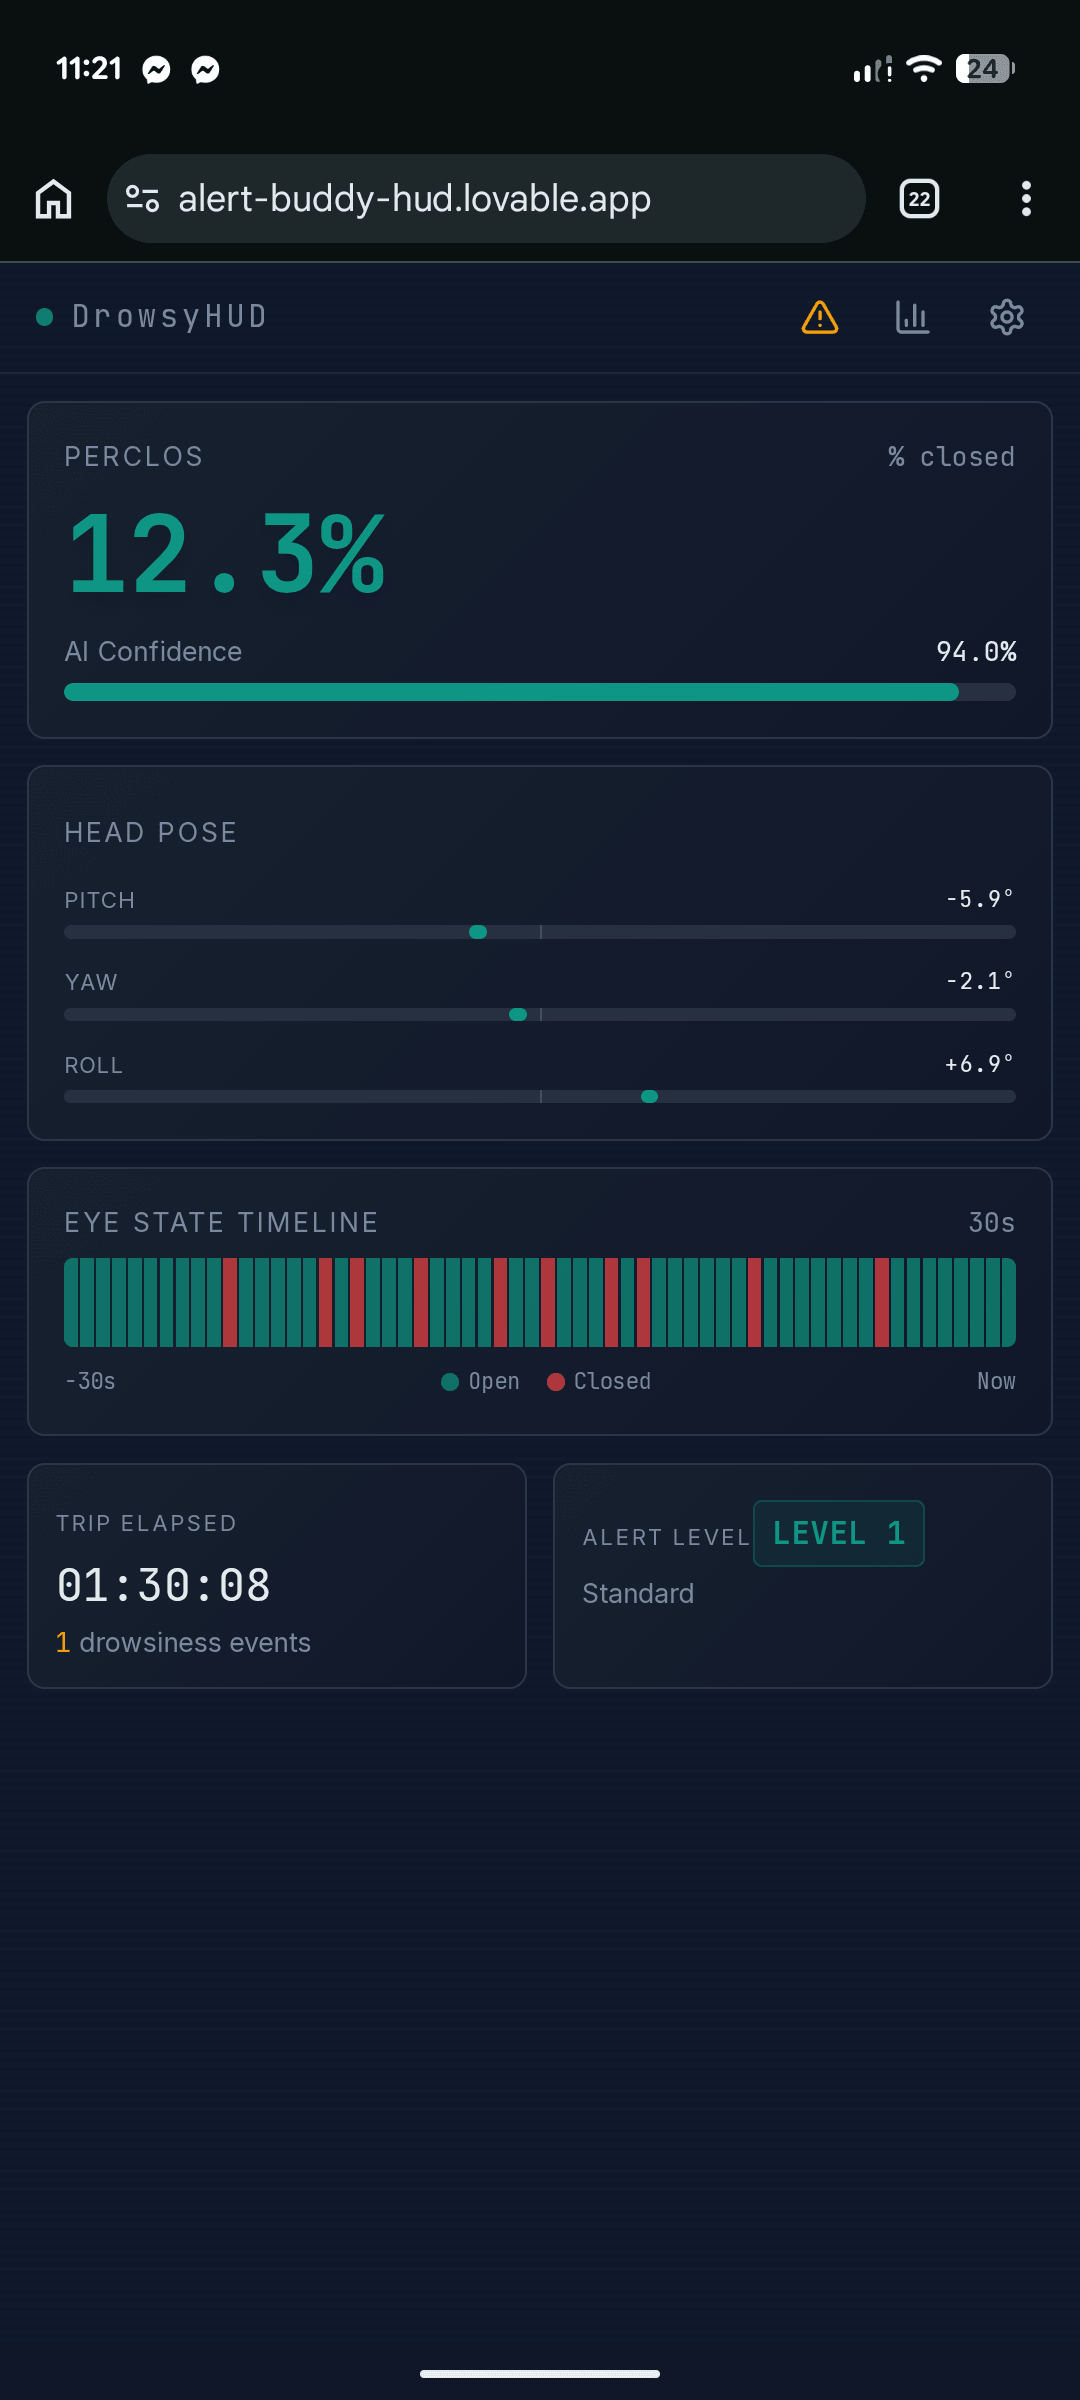
\includegraphics[height=5.5cm]{figures/DrowsyHUD-Monitoring.png}\hfill
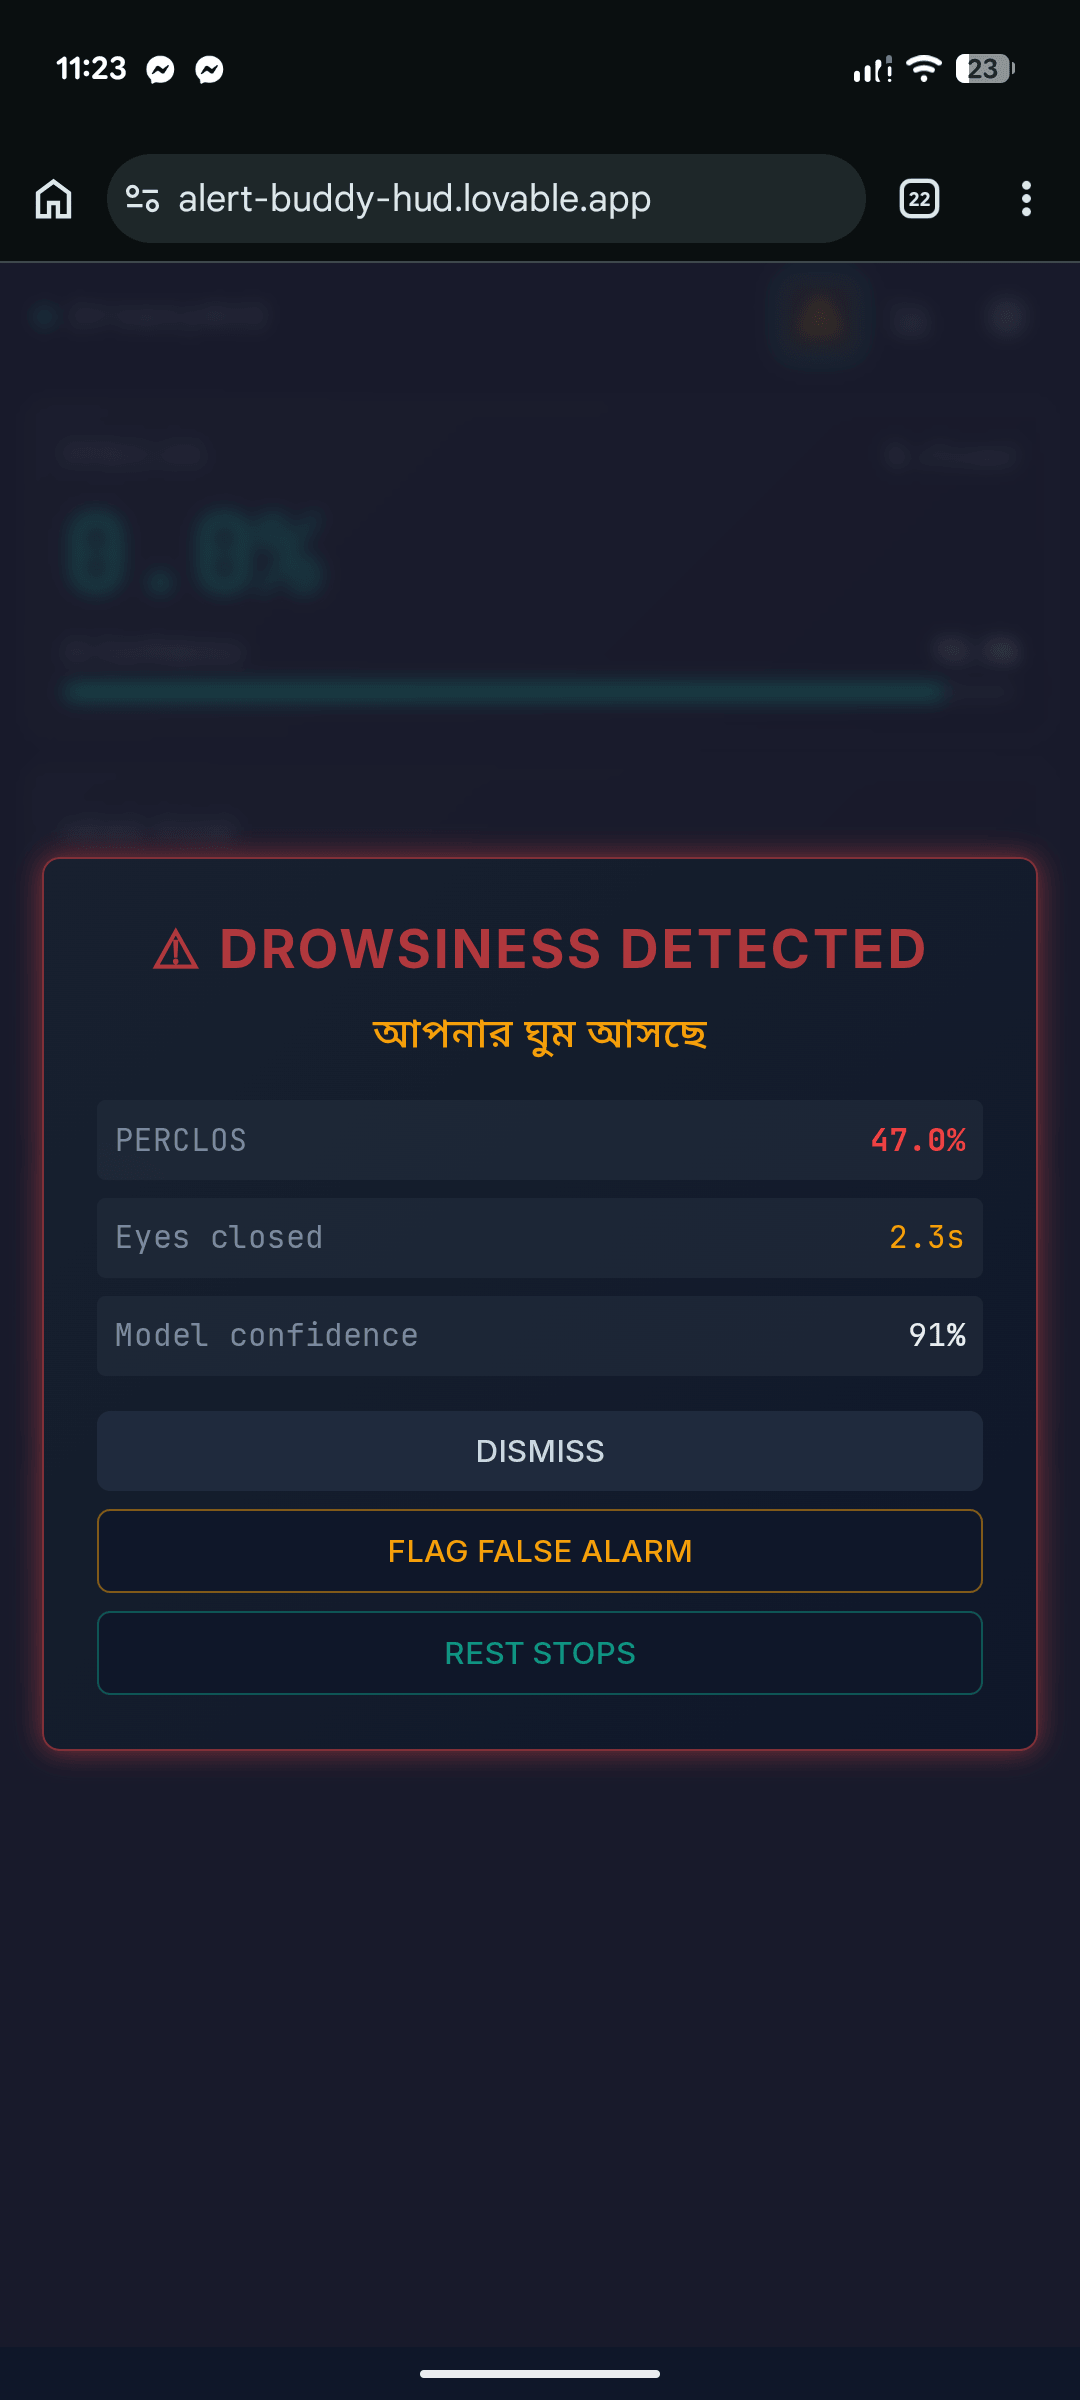
\includegraphics[height=5.5cm]{figures/DrowsyHUD-Alert.png}\hfill
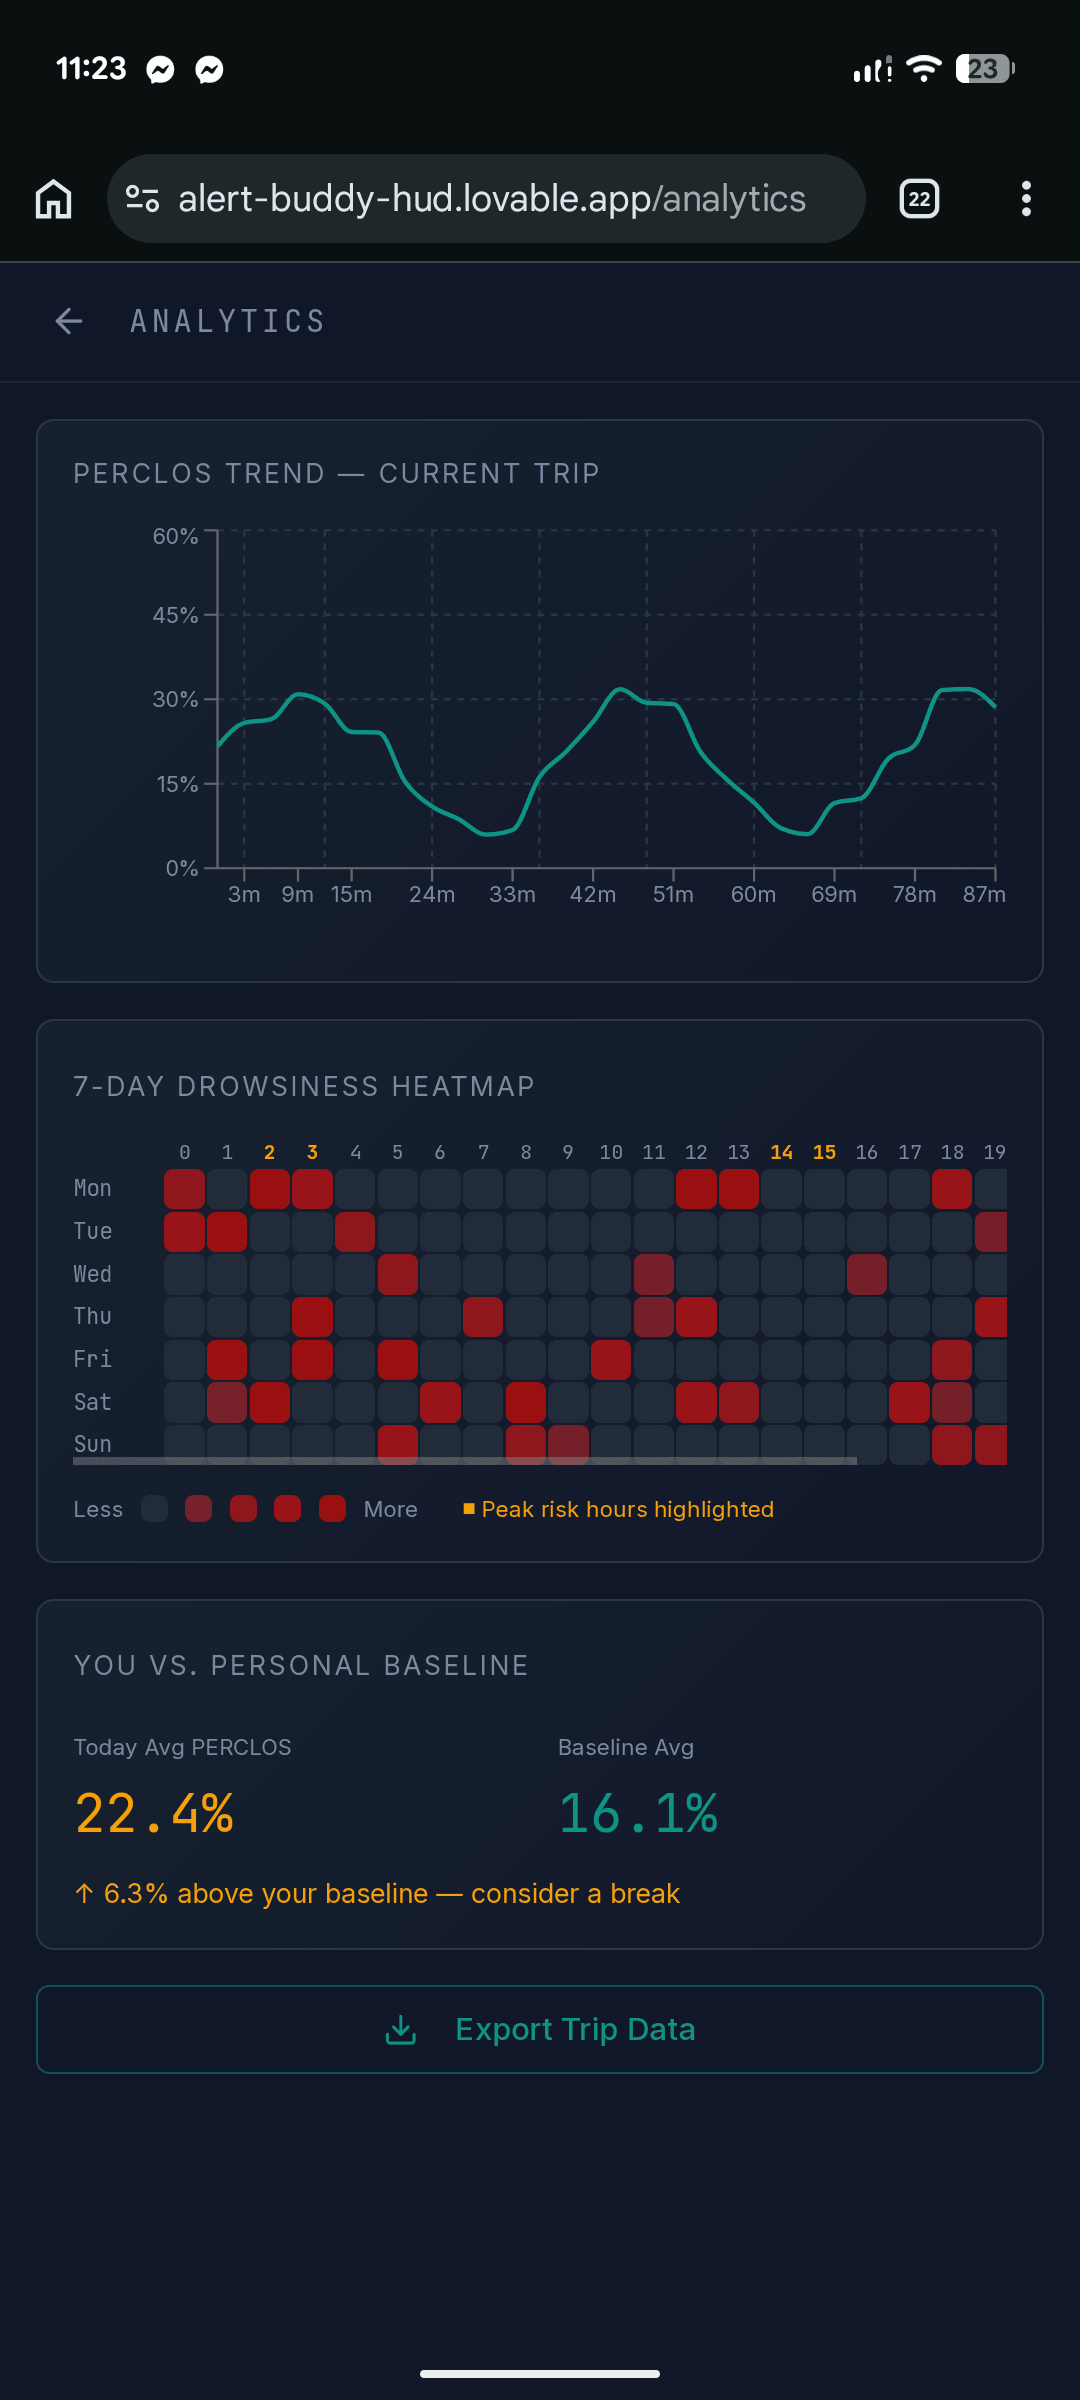
\includegraphics[height=5.5cm]{figures/DrowsyHUD-Heatmap.png}\hfill
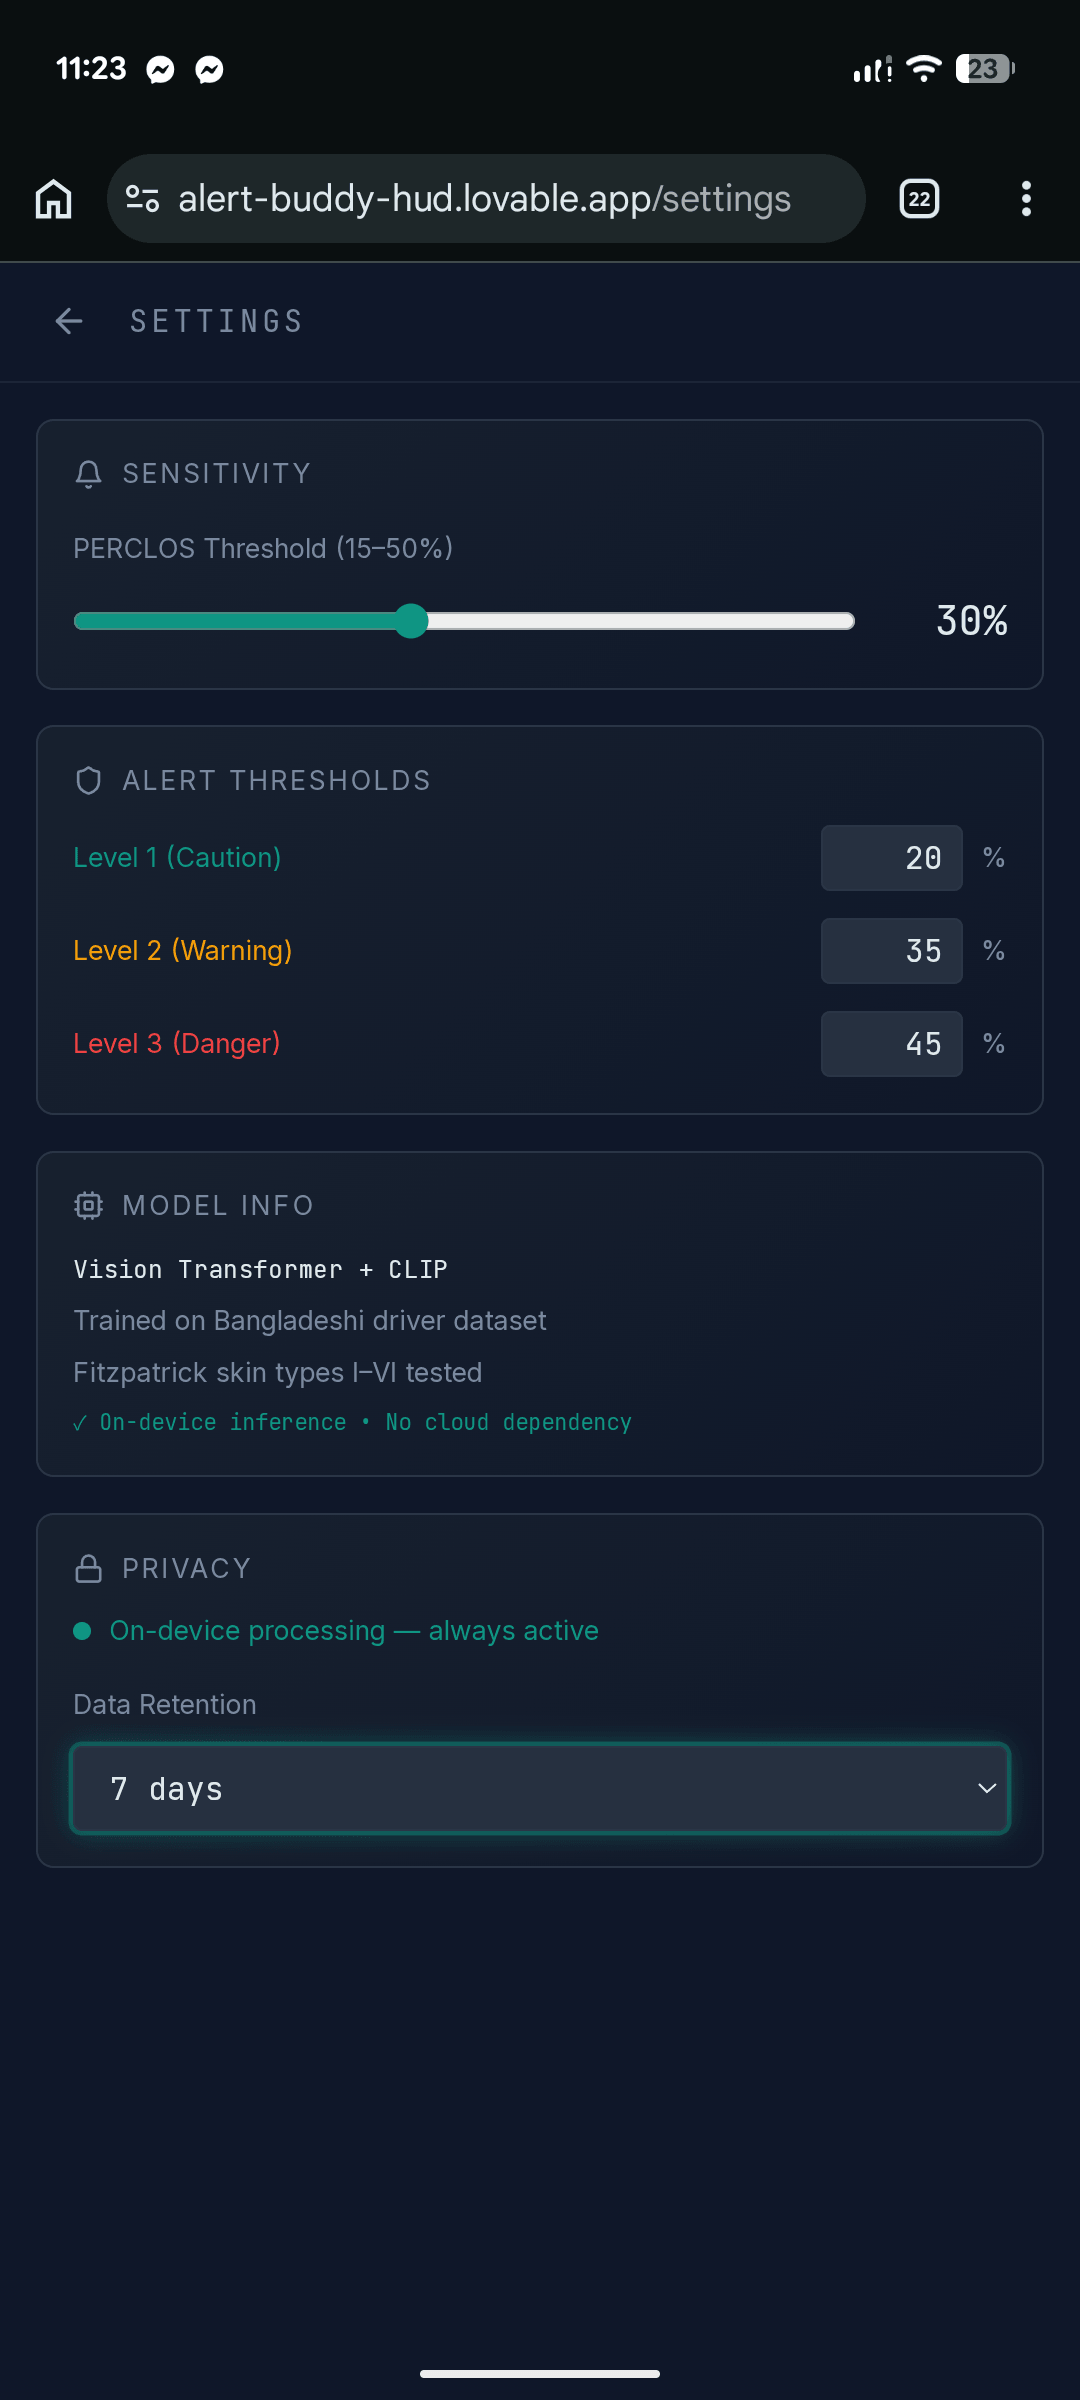
\includegraphics[height=5.5cm]{figures/DrowsyHUD-Settings.png}

\footnotesize\textbf{Source:} \url{https://alert-buddy-hud.lovable.app}
\caption{Design~3 --- DrowsyHUD (Technical HUD Mode) targeting Persona~3 (Fatema). The instrument-panel layout exposes every detection metric in real time: PERCLOS bar, scrolling eye state timeline, EAR and blink rate needle gauges, three-axis head pose indicators, and AI confidence with model identifier. The 7$\times$24 heatmap in analytics enables pattern discovery.}
\label{fig:design3}
\end{figure*}

\paragraph{HCAI Principle Implementation in Design~3}
Table~\ref{tab:hcai_d3} maps HCAI principles to specific features in the DrowsyHUD interface.

\begin{table}[h]
\centering
\caption{HCAI Principles in Design~3 (DrowsyHUD)}
\label{tab:hcai_d3}
\small
\begin{tabular}{|p{2cm}|p{5.5cm}|}
\hline
\textbf{Principle} & \textbf{Implementation} \\
\hline
Transparency & All metrics visible in real time; model architecture disclosed \\
\hline
Explainability & Exact values with thresholds: ``PERCLOS 45.2\%, threshold 40\%'' \\
\hline
Reliability & All indicators independently visible for cross-verification \\
\hline
Human Oversight & Acknowledge, flag, export data with consent for post-trip analysis \\
\hline
\end{tabular}
\end{table}

% ================================================================
% SIDE-BY-SIDE COMPARISON
% ================================================================
\subsection{Comparative Interface View}

Figure~\ref{fig:comparison} presents a side-by-side comparison of the three designs during a ``Caution'' state, illustrating how the same underlying detection data (elevated PERCLOS, declining blink rate) is rendered at three distinct levels of complexity to serve three distinct user personas.

\begin{figure*}[t]
\centering
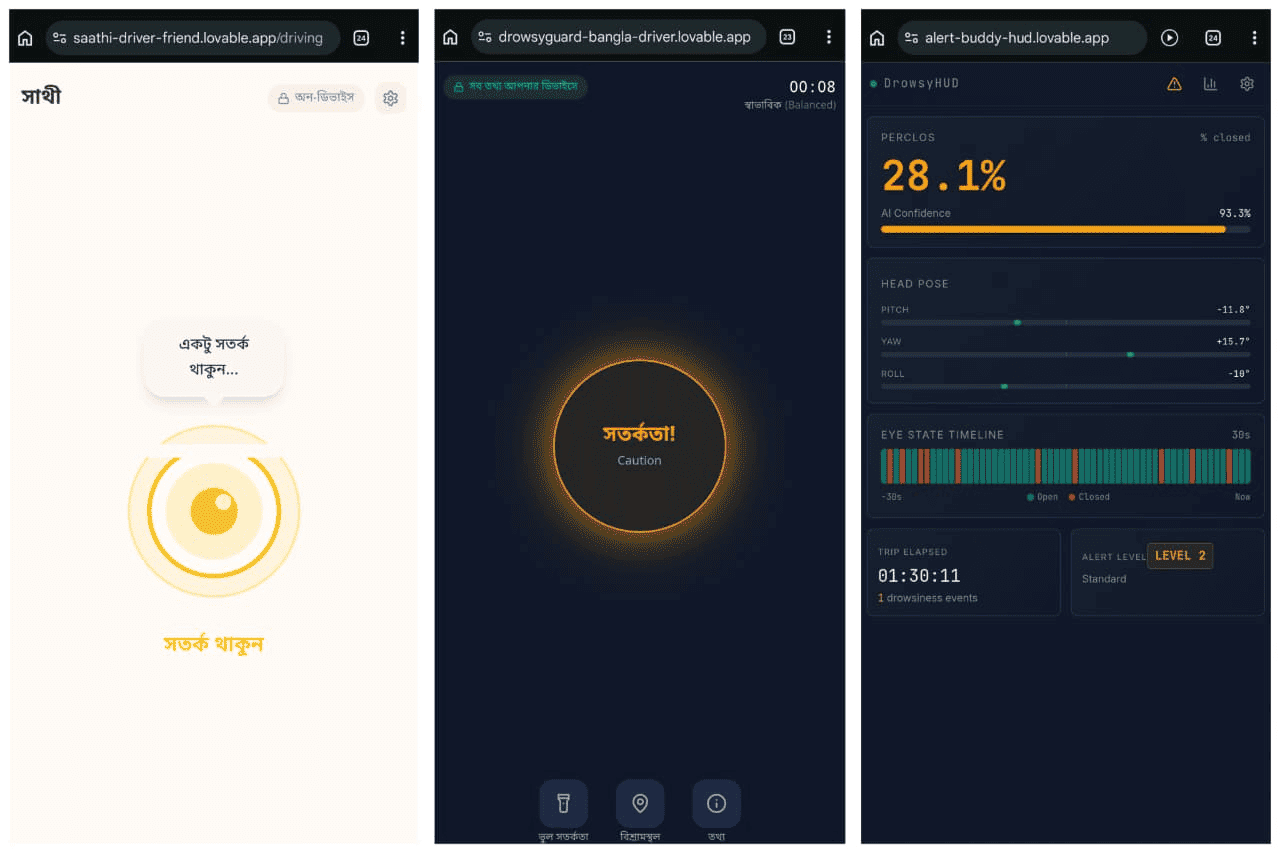
\includegraphics[width=0.95\linewidth]{figures/comparative_interface.png}

\caption{Side-by-side comparison of all three design variants during a ``Caution'' state. The same PERCLOS and EAR data is rendered as: an animated character expression change (left), a color-shifting status indicator (center), and full metric gauges with timeline (right). This demonstrates that HCAI principles of transparency and explainability can be achieved at multiple levels of interface complexity.}
\label{fig:comparison}
\end{figure*}

% ================================================================
% STORYBOARDS AND INTERACTION SCENARIOS
% ================================================================
\subsection{Storyboards and Interaction Scenarios}

The following scenarios demonstrate how users interact with each prototype variant in realistic driving situations. Each scenario was developed from the user needs identified during the requirements analysis and refined through persona analysis.

\paragraph{Scenario 1: Late-Night Drowsiness Onset (Companion Mode --- Rahim)}
Rahim begins his overnight Dhaka-to-Chittagong delivery at 11~PM. After two hours, the system detects decreasing blink rate and increasing PERCLOS. Saathi's expression shifts from \textit{Alert} to \textit{Watching}, with the speech bubble changing to ``Stay a bit careful.'' When PERCLOS exceeds the threshold, Saathi becomes \textit{Worried} and an alert slides up: ``Brother, your eyes are getting heavy. Will you take some rest?'' Rahim taps ``Take rest'' and is shown nearby truck stops with amenity information.

\paragraph{Scenario 2: Highway Monitoring (Dashboard Mode --- Karim)}
Karim drives an intercity bus during a mid-afternoon shift. The Dashboard shows the status indicator in teal (\textit{Monitoring}). After detecting repeated yawning, the indicator shifts to amber (\textit{Caution}) and an alert card appears: ``Repeated yawning detected'' with 91\% confidence. Karim taps ``I'm okay'' and opens the window. Fatigue indicators stabilize and the indicator returns to teal.

\paragraph{Scenario 3: Data-Aware Technical Driving (HUD Mode --- Fatema)}
Fatema drives home from a late meeting. The HUD displays PERCLOS at 18\%, EAR at 0.31, blink rate at 16/min. She notices PERCLOS climbing on the bar. At 45\%, a Level~2 alert triggers: ``PERCLOS threshold exceeded---45.2\% (threshold: 40\%). Eye closure: 2.3s. Blink rate: 8/min.'' She navigates to the nearest rest stop and pulls over. The following week, she reviews the 7$\times$24 heatmap and discovers consistent risk peaks between 10--11~PM.

\paragraph{Scenario 4: False Alarm Handling (All Modes)}
During daylight driving, a momentary sun glare causes incorrect eye closure detection. The driver taps the false alarm flag, logging the event as a false positive. The system acknowledges: ``Thank you, this has been noted.'' This supports the HCAI principle of human oversight by enabling drivers to correct system behavior.

\paragraph{Scenario 5: Smart Break Reminder (All Modes)}
After 2 hours of continuous driving, the system generates a proactive break reminder independent of drowsiness detection: ``You have been driving for 2 hours. Take a break.'' This feature addresses proactive fatigue prevention identified in the survey and operates on a configurable time-based schedule.

\paragraph{Scenario 6: Emergency Contact Escalation (All Modes)}
If a Level~3 (Danger) alert is dismissed three times within 10 minutes, the system offers to send an automated SMS to a pre-configured emergency contact: ``I'm tired in the car. Location: [GPS].'' This feature requires explicit opt-in during setup and addresses the survey finding that drivers want safety nets without constant surveillance.


\section{Unified Prototype: Mode-Switching Architecture}
 
\subsection{Motivation for Unification}
 
The formative evaluation of the three standalone prototypes (Sections~7.2--7.4) revealed a fundamental design tension: each variant excelled for its target persona but left the other two user groups underserved. DrowsyGuard provided balanced information density but lacked the emotional accessibility needed by low-literacy drivers. Saathi built trust through conversational warmth but concealed detection details that tech-savvy drivers demanded. DrowsyHUD offered full metric transparency but overwhelmed users with limited technology experience.
 
A requirements traceability analysis (Table~\ref{tab:traceability}) confirmed that no single variant achieved complete coverage of the eight core requirements identified during the formative requirements analysis. For example, the Companion Mode fully satisfied explainability in Bangla and trust-building but scored as ``partial'' on metric transparency and data export. Conversely, the HUD Mode fully satisfied transparency and export but scored as ``partial'' on learnability and cultural sensitivity. These complementary coverage patterns motivated a unification strategy: rather than selecting one variant as the default, all three interaction paradigms would be preserved within a single application through a mode-switching architecture.
 
\begin{table}[h]
\caption{Requirements Traceability: Standalone Prototype Variants}
\label{tab:traceability}
\centering
\small
\begin{tabular}{lccc}
\toprule
\textbf{Requirement} & \textbf{Companion} & \textbf{Dashboard} & \textbf{HUD} \\
\midrule
Facial Monitoring        & \checkmark & \checkmark & \checkmark \\
Eye Closure (EAR)        & \checkmark & \checkmark & \checkmark \\
Yawning Detection        & \checkmark & \checkmark & \checkmark \\
Head Pose Monitoring     & Partial    & \checkmark & \checkmark \\
Real-time Alert          & \checkmark & \checkmark & \checkmark \\
Bangla Explanation       & \checkmark & \checkmark & Partial    \\
Privacy (On-device)      & \checkmark & \checkmark & \checkmark \\
Metric Transparency      & --         & Partial    & \checkmark \\
Data Export              & --         & --         & \checkmark \\
Learnability             & \checkmark & Partial    & --         \\
Cultural Sensitivity     & \checkmark & Partial    & --         \\
Composite Fatigue Score  & Hidden     & Partial    & \checkmark \\
Break Reminders          & --         & --         & --         \\
Emergency Escalation     & --         & --         & --         \\
\bottomrule
\end{tabular}
\end{table}

 
\subsection{Unified Build Prompt as Design Specification}
 
Following the same methodology used for the three standalone variants, the unified prototype was built using Lovable AI from a comprehensive build prompt treated as a formal design specification. The unified prompt was engineered as a single markdown document of approximately 4{,}500 words specifying every screen, component, state transition, animation sequence, bilingual content string, and interaction pattern across all three modes. Due to its length, the verbatim prompt is presented below in five thematic parts; in practice, these were concatenated into a single document provided to Lovable AI. All user-facing strings were specified in both Bangla (Bengali script) and English in the original prompt; English translations are shown below with \textbf{[Bangla]} markers for typesetting compatibility.
 
\paragraph{Lovable AI Build Prompt (Verbatim)}
 
% ----------------------------------------------------------------
% PART 1: Architecture, Tech Stack, Design System & App State
% ----------------------------------------------------------------
\begin{promptbox}[Prompt~4 (Part~1 of~5): Architecture, Tech Stack, Design System \& App State]
Build a full-stack mobile-first web app called ``DrowsyGuard'' --- an AI-powered real-time driver drowsiness detection system designed for Bangladeshi professional drivers. The app must support three switchable interface modes (Companion Mode, Dashboard Mode, HUD Mode), complete onboarding, real-time detection simulation, alert system, rest stop finder, analytics, weekly summaries, and a comprehensive settings panel. The app is bilingual: primary language is Bangla (Bengali script) with English subtitles everywhere. The entire app must be a single cohesive React application with shared state, routing, and persistent local state using Zustand.
 
\textbf{TECH STACK:} React + TypeScript + Vite. Tailwind CSS with custom theme tokens. React Router v6 (hash-based for mobile compatibility). Zustand for state management. Recharts for analytics. Framer Motion for transitions, character animations, alert pulses. Lucide React icons. Fonts: Noto Sans Bengali (Bangla text), JetBrains Mono (numeric/HUD data), Inter (English UI labels). In-memory state with simulated persistence (no localStorage).
 
\textbf{COLOR TOKENS (Tailwind config):} \texttt{bg-dark: \#0F172A} (deep navy --- dark mode/HUD/driving), \texttt{bg-warm: \#FFFBF7} (warm white --- companion), \texttt{primary: \#0D9488} (electric teal --- safe/active), \texttt{primary-light: \#14B8A6} (teal highlight), \texttt{warning: \#F59E0B} (amber --- caution), \texttt{danger: \#EF4444} (red --- danger), \texttt{alert-coral: \#E8571A} (coral --- alert cards/CTAs), \texttt{alert-soft: \#FF7043} (soft coral --- companion alerts), \texttt{surface: \#1E293B} (card dark), \texttt{surface-light: \#F1F5F9} (card light), \texttt{text-primary: \#F8FAFC} (white on dark), \texttt{text-dark: \#1E293B} (dark on light), \texttt{text-muted: \#94A3B8} (secondary).
 
\textbf{TYPOGRAPHY:} Bangla headings: Noto Sans Bengali, 24px bold. Bangla body: 18px minimum (accessibility for non-tech-savvy drivers). English subtitles: Inter, 14px, muted. HUD numerics: JetBrains Mono, varying sizes. Minimum tap target: 48$\times$48px. Border radius: 16px default, 24px companion cards.
 
\textbf{ACCESSIBILITY:} High contrast by default (WCAG AAA). Large text, bold indicators. No thin fonts or low-opacity text on critical elements. All status colors must also have icon/shape differentiation (not color-only).
 
\textbf{ROUTING:} \texttt{/} $\rightarrow$ Splash/Onboarding (first launch) or redirect to /drive; \texttt{/onboarding} $\rightarrow$ 3-step flow; \texttt{/drive} $\rightarrow$ main driving screen (renders by mode); \texttt{/drive/alert} $\rightarrow$ alert overlay modal; \texttt{/rest-stops} $\rightarrow$ rest stop finder; \texttt{/analytics} $\rightarrow$ PIN-protected weekly summary; \texttt{/settings} $\rightarrow$ full settings panel.
 
\textbf{GLOBAL STATE (Zustand store):} User preferences: \texttt{interfaceMode} (companion/dashboard/hud), \texttt{sensitivity} (conservative/balanced/relaxed), \texttt{perclosThreshold} (15--50, default 30), language (bn/en), \texttt{onboardingComplete}, \texttt{analyticsPIN} (default ``1234''). Privacy: \texttt{deleteDataAfterTrip} (true), \texttt{insuranceSharing} (false), \texttt{employerSharing} (false), \texttt{dataRetention} (end-of-trip/7d/30d/never). Trip: \texttt{tripActive}, start time, elapsed seconds, \texttt{drowsinessEvents[]} array, \texttt{currentAlertLevel} (0--3). Detection: \texttt{perclosScore} (0--100), \texttt{eyeAspectRatio} (0.0--0.5), \texttt{blinkRate}, \texttt{headPose} (pitch/yaw/roll), \texttt{aiConfidence} (0--100), \texttt{eyeState} (open/closing/closed), \texttt{eyeStateTimeline} (last 30s). Weekly: daily events, 7$\times$24 heatmap, peak risk times, stats, tip, week score (1--5 smiley). Night mode flag.
\end{promptbox}
 
 
% ----------------------------------------------------------------
% PART 2: Onboarding, Simulation Engine & Companion Mode
% ----------------------------------------------------------------
\begin{promptbox}[Prompt~4 (Part~2 of~5): Onboarding, Simulation Engine \& Companion Mode]
\textbf{SPLASH (2 seconds):} Dark background (\#0F172A). Stylized eye icon in teal with ``DrowsyGuard'' text. Bangla subtitle: ``Your safety, our commitment'' \textbf{[Bangla]}. Fade to onboarding.
 
\textbf{ONBOARDING SCREEN~1 --- Introduction:} Animated Saathi character (circular eye, line-art, teal) blinks gently. Speech bubble: ``I am Saathi. I will stay by your side in your car'' \textbf{[Bangla]}. English subtitle: ``I'm Saathi, your driving companion.'' ``Next'' \textbf{[Bangla]} button.
 
\textbf{ONBOARDING SCREEN~2 --- Privacy Promise:} Lock icon animation (closing). Text: ``I work only on your phone. Your images don't go anywhere'' \textbf{[Bangla]}. English: ``100\% on-device processing. No images leave your phone.'' Phone-with-shield visual, data flowing inside phone only. Badges: ``No cloud'' \textbf{[Bangla]}, ``No tracking'' \textbf{[Bangla]}.
 
\textbf{ONBOARDING SCREEN~3 --- Choose Experience:} Two selection groups. \textit{Sensitivity:} Three illustrated cards (tap to select, teal border) --- ``Extra Careful'' \textbf{[Bangla]}: ``Will alert on small signs'' \textbf{[Bangla]}; ``Balanced'' \textbf{[Bangla]} (default): ``Balanced monitoring'' \textbf{[Bangla]}; ``Relaxed'' \textbf{[Bangla]}: ``Only on clear signs'' \textbf{[Bangla]}. \textit{Interface Mode:} Three cards with previews --- ``Companion Mode'' \textbf{[Bangla]}: ``Like a friend'' \textbf{[Bangla]} (default); ``Dashboard Mode'' \textbf{[Bangla]}: ``Clear information'' \textbf{[Bangla]}; ``HUD Mode'' \textbf{[Bangla]}: ``Detailed data'' \textbf{[Bangla]}. ``Start'' \textbf{[Bangla]} button $\rightarrow$ /drive.
 
\textbf{SIMULATION ENGINE (\texttt{useDrowsinessSimulation} hook):} Shared across all modes. Timer updates every second. Gradually increases PERCLOS from 5\% to random peaks. Every 45--90s triggers drowsiness event with random severity. Updates eye state timeline (last 30s of open/closed segments). Subtle head pose drift. Blink rate: 15--20/min normal, 5--10/min drowsy. AI confidence: 85--98\%. Alert when PERCLOS exceeds threshold or eye closure $>$2s.
 
\textbf{COMPANION MODE (Drive Screen):} Background: warm white (\#FFFBF7). Top bar: tiny lock icon (teal, tappable, shows ``All data on your device'' \textbf{[Bangla]} tooltip) + trip timer in dark text + sensitivity badge. Center (60\%): Saathi character --- large animated circular eye (150px). States with Framer Motion transitions: \textit{Alert} (PERCLOS 0--20\%): bright open eye, teal iris, idle blink 3--4s, slight bounce; \textit{Watching} (21--40\%): slightly narrowed, amber iris, increased blink, side-to-side look; \textit{Worried} (41--60\%): drooping upper eyelid (half-closed), coral iris, soft pulse glow; \textit{Critical} (61\%+): heavy drooping lid, red iris, shaking/vibration, red pulse ring expanding. Speech bubble (24px radius, light shadow) rotates every 30s: Alert: ``You're doing great! Drive safe'' / ``All good, stay focused'' / ``Excellent! Keep going'' \textbf{[Bangla]}. Watching: ``Stay a bit careful'' / ``Open the window a bit'' \textbf{[Bangla]}. Worried: ``Brother, will you take some rest?'' / ``You seem tired'' \textbf{[Bangla]}. Critical: direct alert triggers. Bottom status (22px bold): ``Safe'' \textbf{[Bangla]} (teal) / ``Stay alert'' \textbf{[Bangla]} (amber) / ``Take rest'' \textbf{[Bangla]} (coral). Bottom navigation (3 icons, 56px): false alarm flag ``False alarm'' \textbf{[Bangla]}, map pin ``Rest place'' \textbf{[Bangla]}, info ``Why did I alert?'' \textbf{[Bangla]}.
\end{promptbox}
 
 
% ----------------------------------------------------------------
% PART 3: Dashboard Mode, HUD Mode & Alert System
% ----------------------------------------------------------------
\begin{promptbox}[Prompt~4 (Part~3 of~5): Dashboard Mode, HUD Mode \& Alert System]
\textbf{DASHBOARD MODE (Drive Screen):} Background: dark (\#0F172A). Top bar: green privacy badge with lock ``All data on your device'' \textbf{[Bangla]} + trip timer + sensitivity label (Conservative/Balanced/Relaxed) \textbf{[Bangla]}. Center: large circular status indicator (200px). States: \textit{Monitoring} (safe): teal glow, ``Monitoring'' \textbf{[Bangla]} text, breathing pulse; \textit{Caution}: amber ring, 1.5s pulse, ``Caution!'' \textbf{[Bangla]}; \textit{Danger}: red ring, 0.8s pulse, ``Danger!'' \textbf{[Bangla]}, red vignette. Inside: PERCLOS \% large + AI confidence below. Quick stats row (4 cards): blink rate, eye state (``Eyes: open'' / ``Eyes: closing'' \textbf{[Bangla]}), head pose arrow, event count. Same 3 bottom buttons (dark theme).
 
\textbf{HUD MODE (Drive Screen):} Background: deep navy (\#0F172A), cockpit/aviation aesthetic. Top: PERCLOS in JetBrains Mono 48px (0--20\% teal, 21--40\% amber, 41\%+ red with pulse) + AI confidence with animated teal bar + alert level badge (Level 0/1/2/3). Center: eye state timeline --- horizontal bar (last 30s), each second = rect (teal=open, red=closed, amber=closing), scrolls left, current second highlighted. Right: three circular gauges (60px) vertically --- Pitch ($-30$\textdegree{} to $+30$\textdegree), Yaw ($-45$\textdegree{} to $+45$\textdegree), Roll ($-20$\textdegree{} to $+20$\textdegree), needle indicators (teal centered, amber $>$15\textdegree, red $>$25\textdegree). Bottom bar: trip time \textbf{[Bangla]} + event count \textbf{[Bangla]}, EAR value + blink rate, sensitivity + threshold \textbf{[Bangla]}.
 
\textbf{ALERT TRIGGERS (simulated):} PERCLOS exceeds user-set threshold (default 30\%); eye closure $>$2s; blink rate $<$8/min for $>$30s; head pose deviation $>$25\textdegree{} sustained $>$5s.
 
\textbf{COMPANION ALERT:} Saathi bounces (scale 1.0$\rightarrow$1.3$\rightarrow$1.0, spring physics), eye goes wide then concerned. Speech bubble: ``Brother, be careful. Your eyes were closing'' / ``Your head is dropping! Be careful!'' / ``Your eyes are getting heavy'' \textbf{[Bangla]}. English subtitle below. Two stacked buttons (56px, full-width): ``I'm okay, thanks'' \textbf{[Bangla]} (outline, dismiss) / ``I need rest'' \textbf{[Bangla]} (coral, $\rightarrow$ rest stops). On dismiss: ``Okay, I'm watching!'' \textbf{[Bangla]}. On false alarm flag: ``Was this wrong? Okay, I'll remember!'' \textbf{[Bangla]}.
 
\textbf{DASHBOARD ALERT:} White card slides up (Framer Motion spring). Coral (\#E8571A) top border 4px. Drowsy eye SVG icon. Bangla reason (24px bold): ``Your eyes are getting heavy'' \textbf{[Bangla]}. English detail (14px): ``Eyes closing detected --- PERCLOS reached 47\%.'' Confidence bar: ``Confidence: 87\%'' \textbf{[Bangla]} with teal fill. Side-by-side: ``I'm okay'' \textbf{[Bangla]} (outline) / ``Take rest'' \textbf{[Bangla]} (coral). Swipe down to dismiss.
 
\textbf{HUD ALERT:} Red overlay (10\% opacity) pulses 3$\times$. Center modal (dark surface): ``DROWSINESS DETECTED'' (red, 28px). Data grid: ``PERCLOS: 47\%,'' ``Eye closure: 2.3s,'' ``Model confidence: 91\%,'' ``Blink rate: 6/min.'' Bangla secondary: ``You are getting drowsy'' \textbf{[Bangla]}. Three buttons: DISMISS / FLAG FALSE ALARM / SHOW REST STOPS. Auto-adds to event timeline.
\end{promptbox}
 
 
% ----------------------------------------------------------------
% PART 4: Rest Stops, Analytics & Settings
% ----------------------------------------------------------------
\begin{promptbox}[Prompt~4 (Part~4 of~5): Rest Stops, Analytics \& Settings]
\textbf{REST STOP FINDER:} Header: ``Nearby Rest Places'' \textbf{[Bangla]} + back arrow. Simulated map area (styled div with road illustration and markers, no Google Maps). Three numbered pins. Cards (white/dark by mode): stop name \textbf{[Bangla]} (e.g., ``Dhaka--Chittagong Rest Area''), distance ``3.5 km'' \textbf{[Bangla]}, drive time ``$\sim$5 minutes'' \textbf{[Bangla]}, amenity icons (toilet/food/fuel/parking). ``Stop here'' \textbf{[Bangla]} button (coral). Confirmation: ``Starting navigation\ldots'' \textbf{[Bangla]}.
 
\textbf{ANALYTICS --- PIN GATE:} ``Enter PIN to view weekly report'' \textbf{[Bangla]}. 4-digit PIN pad, large buttons. Default: 1234.
 
\textbf{ANALYTICS --- COMPANION VERSION:} Saathi with weekly mood. Smiley-face rating (5 = great, 1 = tough). Bangla summary: ``This week you were tired 3 times. Most tiredness after 11 PM'' \textbf{[Bangla]}. Tip: ``Rest 30 minutes before night driving'' \textbf{[Bangla]}.
 
\textbf{ANALYTICS --- DASHBOARD VERSION:} Recharts bar chart (Mon--Sun) \textbf{[Bangla]}. Top~3 risk slots (amber cards). Bangla tip. Share button (disabled, consent dialog on tap).
 
\textbf{ANALYTICS --- HUD VERSION:} 7$\times$24 heatmap (days$\times$hours, color intensity = frequency). PERCLOS trend chart. Peak risk markers (amber). Comparison: ``Your average vs.\ personal baseline'' \textbf{[Bangla]}. Stats table: avg PERCLOS, max closure, event count, avg confidence. Export button $\rightarrow$ consent $\rightarrow$ ``Data exported'' \textbf{[Bangla]}.
 
\textbf{SHARE CONSENT DIALOG:} ``Do you want to share this data?'' \textbf{[Bangla]}. Explanation: ``This will only be shared with your permission'' \textbf{[Bangla]}. ``Share'' / ``Cancel'' \textbf{[Bangla]}.
 
\textbf{COMPANION SETTINGS (``Saathi's Preferences'' [Bangla]):} Saathi asks conversationally: ``How careful should I be?'' \textbf{[Bangla]} $\rightarrow$ 3 sensitivity cards. ``Should I be quieter at night?'' \textbf{[Bangla]} $\rightarrow$ Yes/No. ``Delete all data after trip?'' \textbf{[Bangla]} $\rightarrow$ Yes (default)/No. ``Share with insurance?'' \textbf{[Bangla]} $\rightarrow$ No (default)/Yes with explanation: ``This could reduce your insurance cost, but it's your decision'' \textbf{[Bangla]}. ``Share with employer?'' \textbf{[Bangla]} $\rightarrow$ No (default, locked) with warning: ``If enabled, your employer can see your driving data'' \textbf{[Bangla]}. Language toggle + mode switch.
 
\textbf{DASHBOARD SETTINGS:} Sensitivity (3-button: Conservative/Balanced/Relaxed) \textbf{[Bangla]}. Privacy: insurance (OFF), employer (OFF, locked + warning), on-device badge ``All data on this device'' \textbf{[Bangla]}. Data: delete-after-trip (ON), retention selector. About: Fitzpatrick I--VI card ``This AI works equally on all skin tones'' \textbf{[Bangla]}, model: ``DrowsyCLIP --- Vision Transformer + CLIP Foundation Model,'' ``Trained on Bangladeshi driver data'' \textbf{[Bangla]}. System: off-switch with ``Auto-restarts in 30 seconds'' \textbf{[Bangla]} (30s countdown with red ring), PIN change, version.
 
\textbf{HUD SETTINGS:} All above plus: threshold sliders --- PERCLOS Level~1 (15--50\%, default 25\%), Level~2 (25--60\%, default 35\%), Level~3 (35--70\%, default 45\%), eye closure (1.0--5.0s, default 2.0s), blink rate (4--12/min, default 8/min). Model card: ``ViT-B/16 + CLIP Text Encoder, Cross-Modal Attention Fusion (Q-Former inspired), Temporal Aggregation Transformer, Training: NTHU-DDD, UTA-RLDD, YawDD, Fitzpatrick I--VI validated, On-device $\sim$35 FPS.'' Retention: trip/7d/30d/never. Storage usage.
\end{promptbox}
 
 
% ----------------------------------------------------------------
% PART 5: Additional Features, Navigation, Animations & Requirements
% ----------------------------------------------------------------
\begin{promptbox}[Prompt~4 (Part~5 of~5): Additional Features, Navigation \& Final Requirements]
\textbf{DROWSINESS PREDICTION:} Subtle card on all driving screens: ``Next risk: $\sim$15 minutes'' \textbf{[Bangla]} --- estimates next episode from patterns and time-of-day risk.
 
\textbf{ENVIRONMENTAL CONTEXT:} Auto night mode after sunset (dimmer, warmer). Tip: ``Night driving --- stay extra careful'' \textbf{[Bangla]}. Highway/city toggle (simulated).
 
\textbf{COMPOSITE FATIGUE SCORE:} ``Fatigue Score'' \textbf{[Bangla]} 0--100 combining: PERCLOS (40\%), blink rate deviation (20\%), head pose instability (20\%), time driving without break (20\%). Circular gauge on dashboard/HUD.
 
\textbf{SMART BREAK REMINDERS:} At 2h: ``You've been driving for 2 hours. Take a break'' \textbf{[Bangla]}. At 4h: more urgent amber. Configurable interval.
 
\textbf{EMERGENCY CONTACT:} Settings: add one contact. If Level~3 dismissed 3$\times$ in 10min $\rightarrow$ offer SMS: ``I'm tired in the car. Location: [GPS]'' \textbf{[Bangla]}. Explicit opt-in.
 
\textbf{DRIVER CALIBRATION:} First-time screen: ``Calibrate your normal eye state'' \textbf{[Bangla]}. Instruction: look straight, blink normally 10s. Progress bar. Sets personal EAR + blink baseline.
 
\textbf{AUDIO ALERTS:} Toggle: ``Alert with sound'' \textbf{[Bangla]} (default ON). Chime (L1), beep (L2), alarm (L3). Voice text: ``Careful! You're getting drowsy!'' \textbf{[Bangla]}.
 
\textbf{TRIP HISTORY:} From analytics. Past trips: date, duration, event count, severity breakdown (L1/L2/L3). ``Details'' \textbf{[Bangla]} button $\rightarrow$ trip timeline.
 
\textbf{BOTTOM TAB BAR (persistent):} 4 tabs with icons + Bangla labels: ``Drive'' \textbf{[Bangla]} $\rightarrow$ /drive, ``Rest'' \textbf{[Bangla]} $\rightarrow$ /rest-stops, ``Report'' \textbf{[Bangla]} $\rightarrow$ /analytics, ``Settings'' \textbf{[Bangla]} $\rightarrow$ /settings. Active: teal icon+text. Inactive: muted gray.
 
\textbf{MODE SWITCHER:} Available in settings AND long-press on drive tab. Crossfade 300ms. All state preserved.
 
\textbf{ANIMATIONS:} (1)~Saathi: CSS keyframe blink/concern/worry/critical shake, transform+opacity. (2)~Status ring pulse: box-shadow keyframes. (3)~Alert slide-up: Framer Motion spring. (4)~PERCLOS bar: width transition 1s. (5)~HUD timeline: continuous left-scroll, 1 segment/s. (6)~Gauge needles: transform rotate. (7)~Screen transitions: AnimatePresence fade/slide. (8)~Button press: scale 0.95, spring-back. (9)~Night mode: background crossfade 500ms.
 
\textbf{SIMULATED DATA:} Trip auto-starts on /drive, PERCLOS rises, events at semi-random intervals. Weekly: Mon 0, Tue 1 (11:30 PM), Wed 0, Thu 2 (10:15 PM, 11:45 PM), Fri 1 (3:30 AM), Sat 0, Sun 1 (2:00 AM). Peak risk: ``10 PM--4 AM'' \textbf{[Bangla]}, ``2 PM--3 PM'' \textbf{[Bangla]}. Weekly tip: ``You get more tired after 10 PM. Try to reduce driving or rest 10 minutes every hour'' \textbf{[Bangla]}.
 
\textbf{FINAL REQUIREMENTS:} (1)~Fully functional React app --- all screens navigable, all states work, all animations play. (2)~Responsive 360--428px + tablet. (3)~Bilingual throughout. (4)~Three modes fully implemented, state preserved on switch. (5)~Real-time simulation (PERCLOS, eye state, head pose live). (6)~Alert system end-to-end (trigger, display, dismiss/rest/flag). (7)~Privacy-first: all sharing OFF, delete-after-trip ON, on-device badges prominent. (8)~Accessible: large text, high contrast, large tap targets, no color-only indicators. (9)~No external API calls. (10)~Production-quality typed modular code. Build as complete deployable application. This is a research prototype demonstrating how a DrowsyCLIP-based drowsiness detection system would work as a consumer product for Bangladeshi professional drivers.
\end{promptbox}

 
\noindent The five prompt parts above were concatenated into a single 4{,}500-word markdown document and provided to Lovable AI as a complete build specification. All user-facing strings were specified in both Bangla (Bengali script) and English in the original prompt; English translations are shown above for typesetting compatibility. The technology stack, state management schema, and simulation engine specifications ensured that the generated application was immediately functional upon deployment without manual code modifications.
 
\textbf{Deployment.} The unified prototype is deployed as a live web application accessible at \url{https://drowsiness-detection-pro.lovable.app}, enabling evaluation on actual mobile devices in realistic conditions.


% ================================================================
% UNIFIED PROTOTYPE SCREENSHOTS
% ================================================================
 
\begin{figure*}[t]
\centering
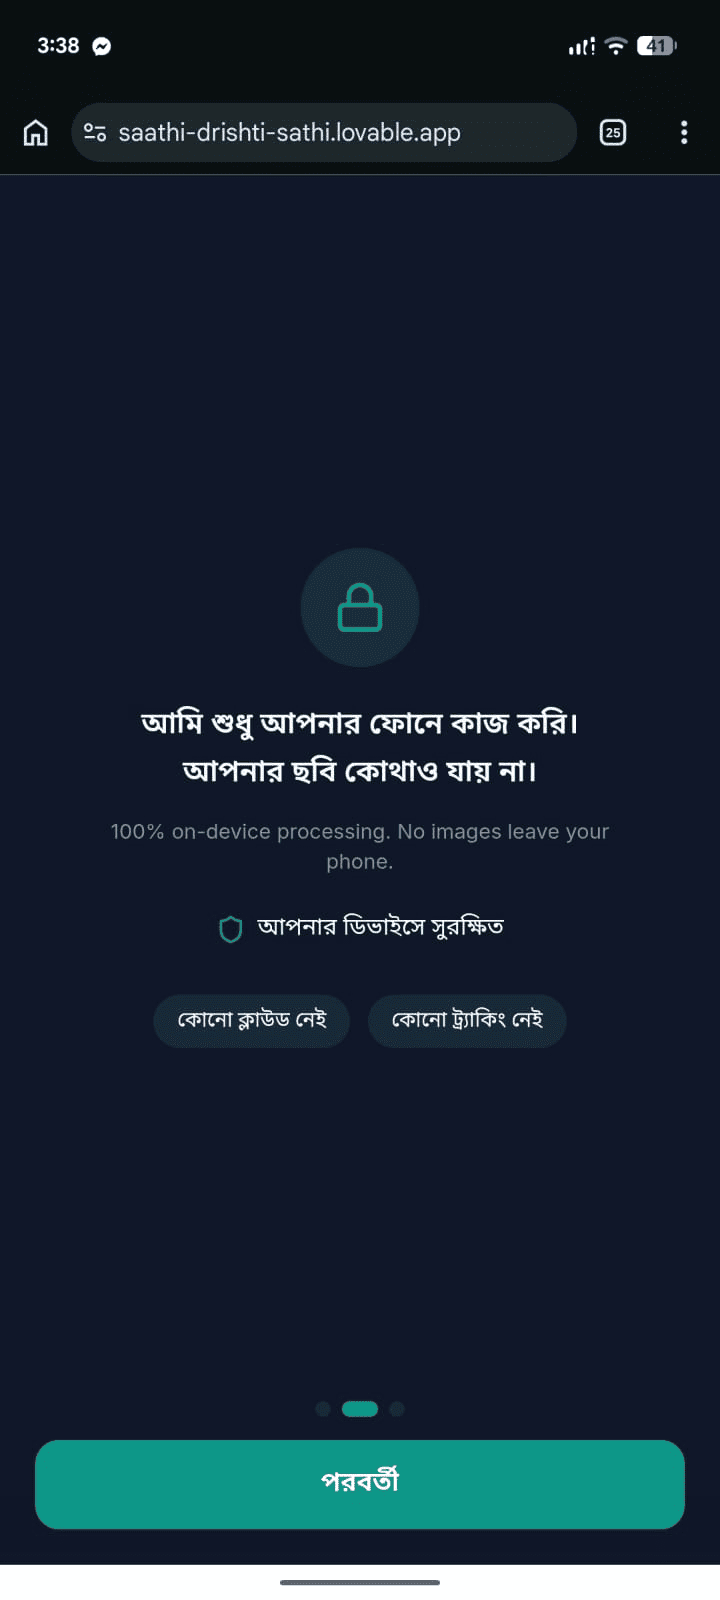
\includegraphics[height=5.5cm]{figures/Unified-Onboarding.png}\hfill
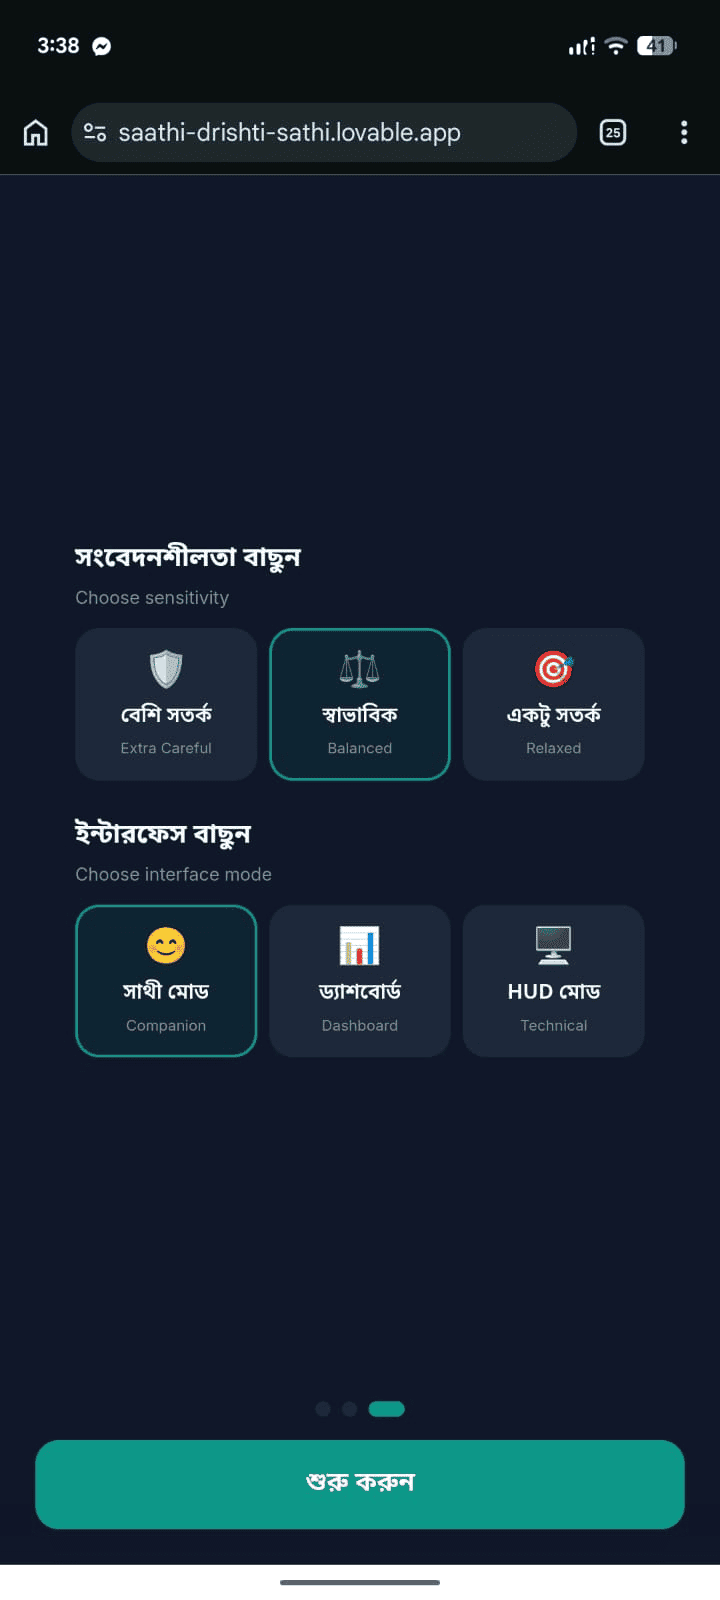
\includegraphics[height=5.5cm]{figures/Unified-ModeSelect.png}\hfill
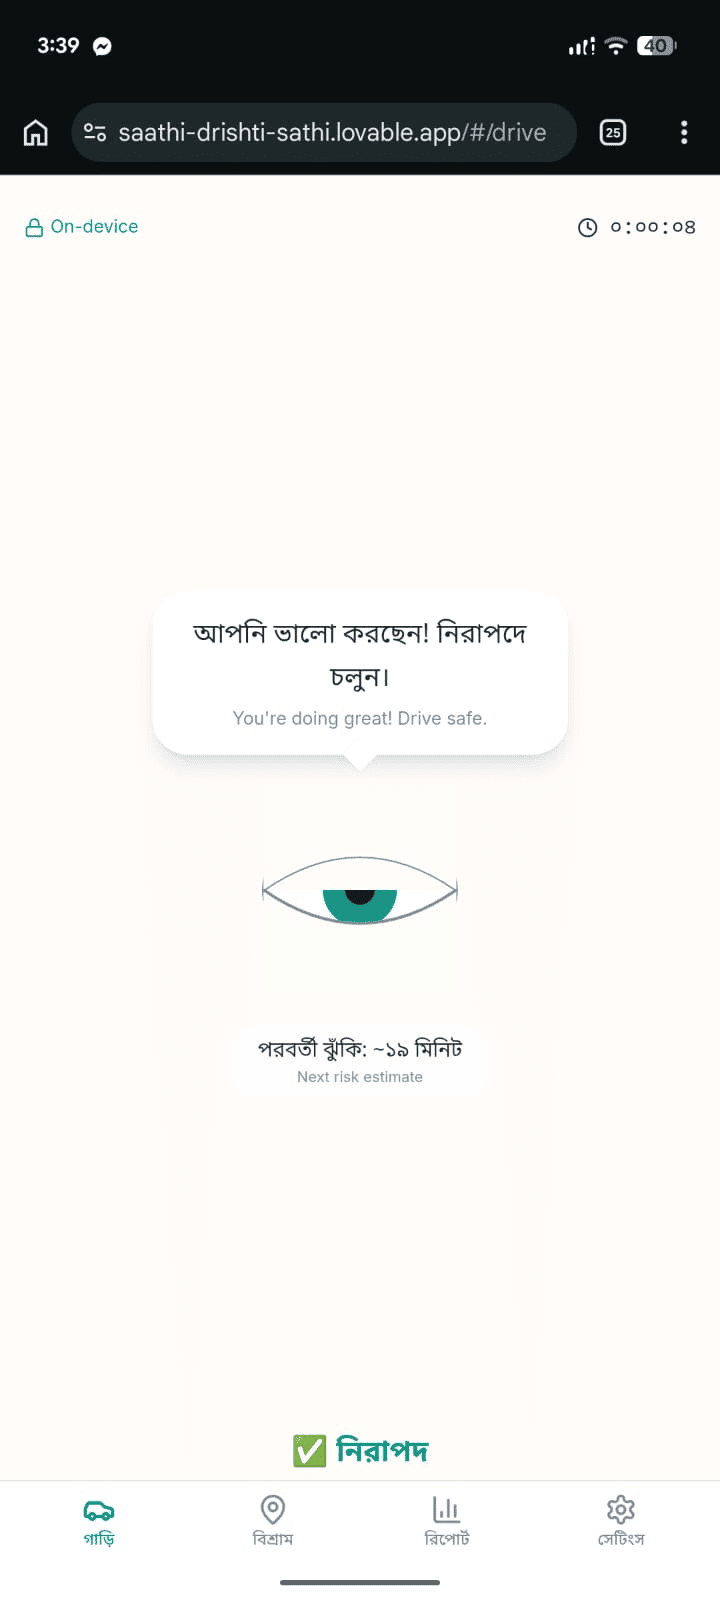
\includegraphics[height=5.5cm]{figures/Unified-Companion-Drive.png}\hfill
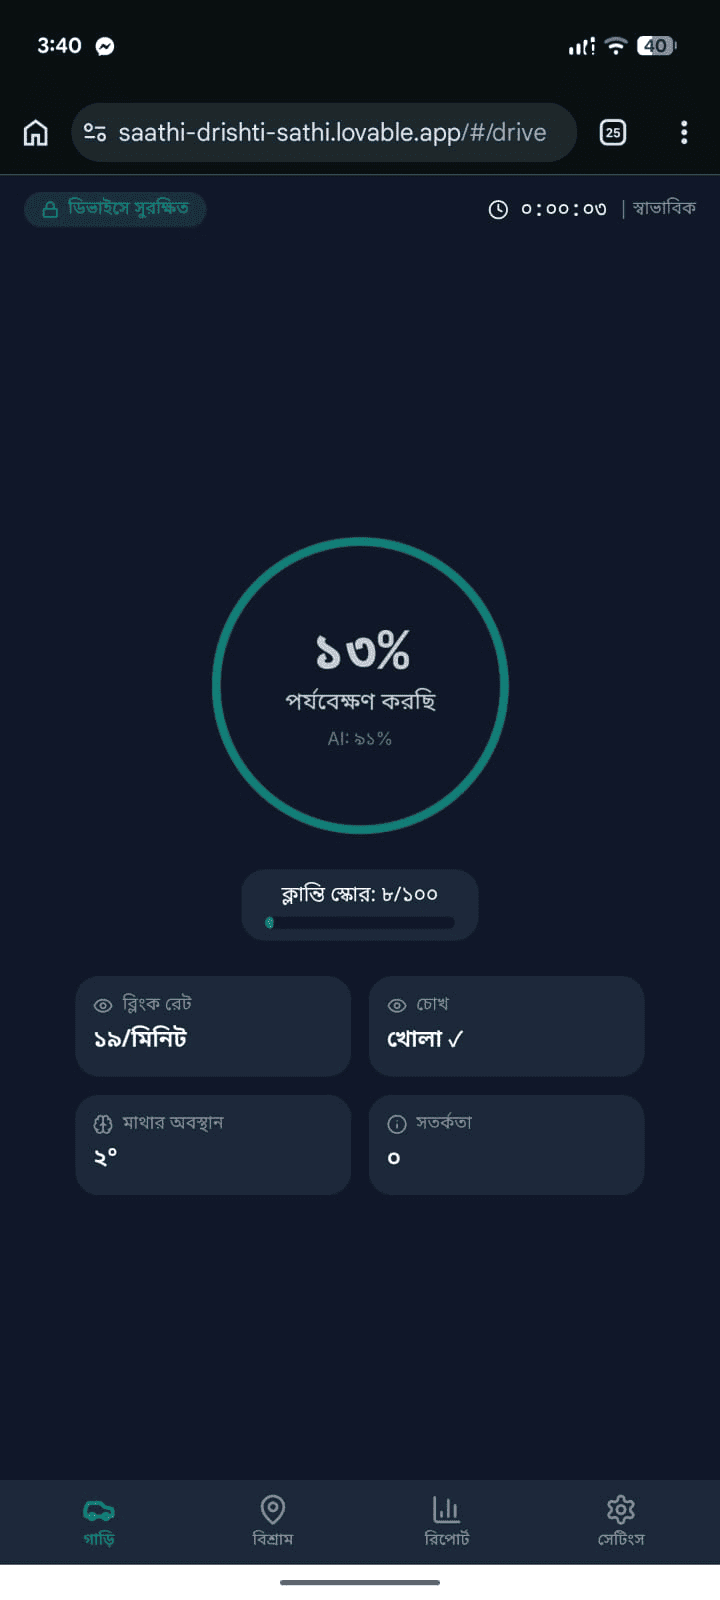
\includegraphics[height=5.5cm]{figures/Unified-Dashboard-Drive.png}\hfill
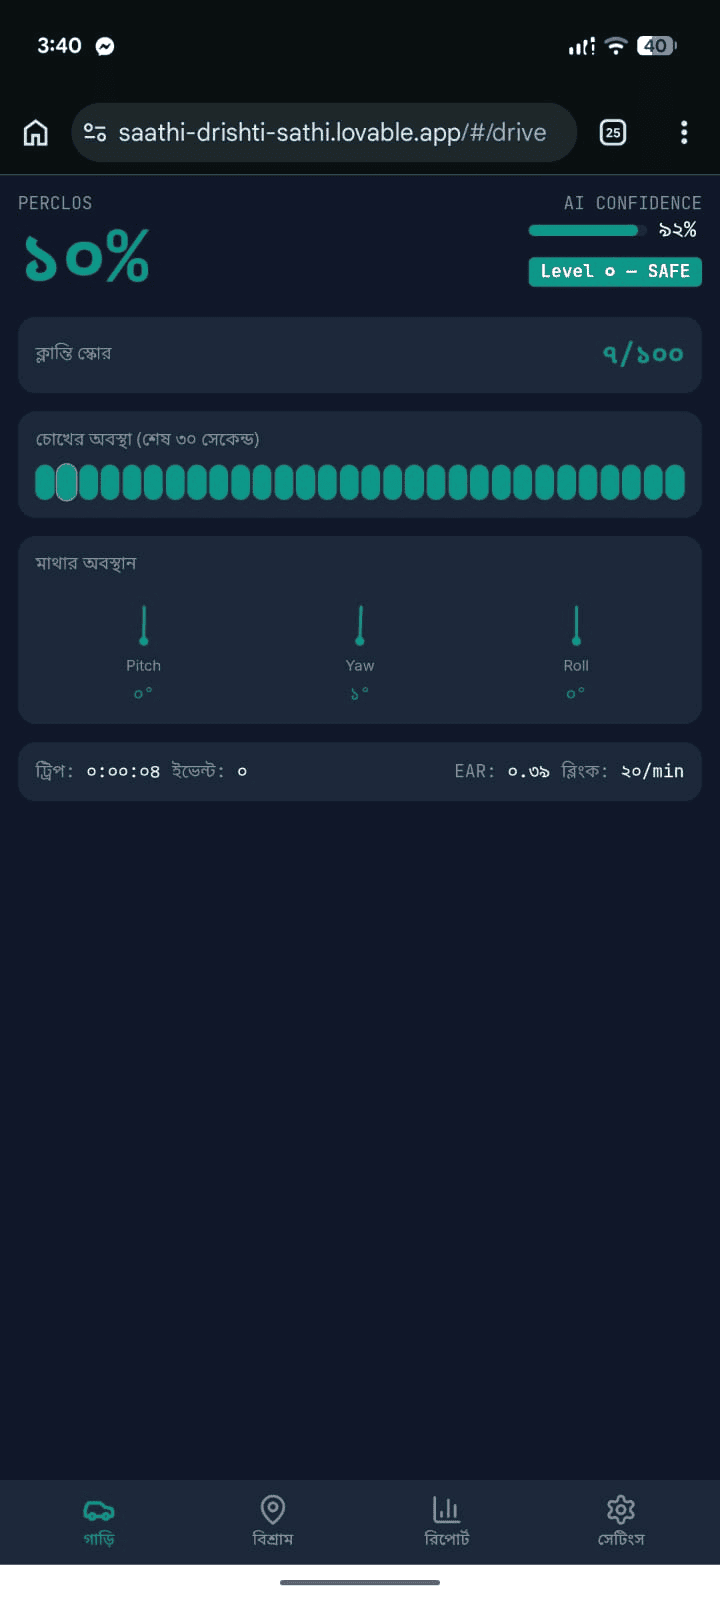
\includegraphics[height=5.5cm]{figures/Unified-HUD-Drive.png}\hfill
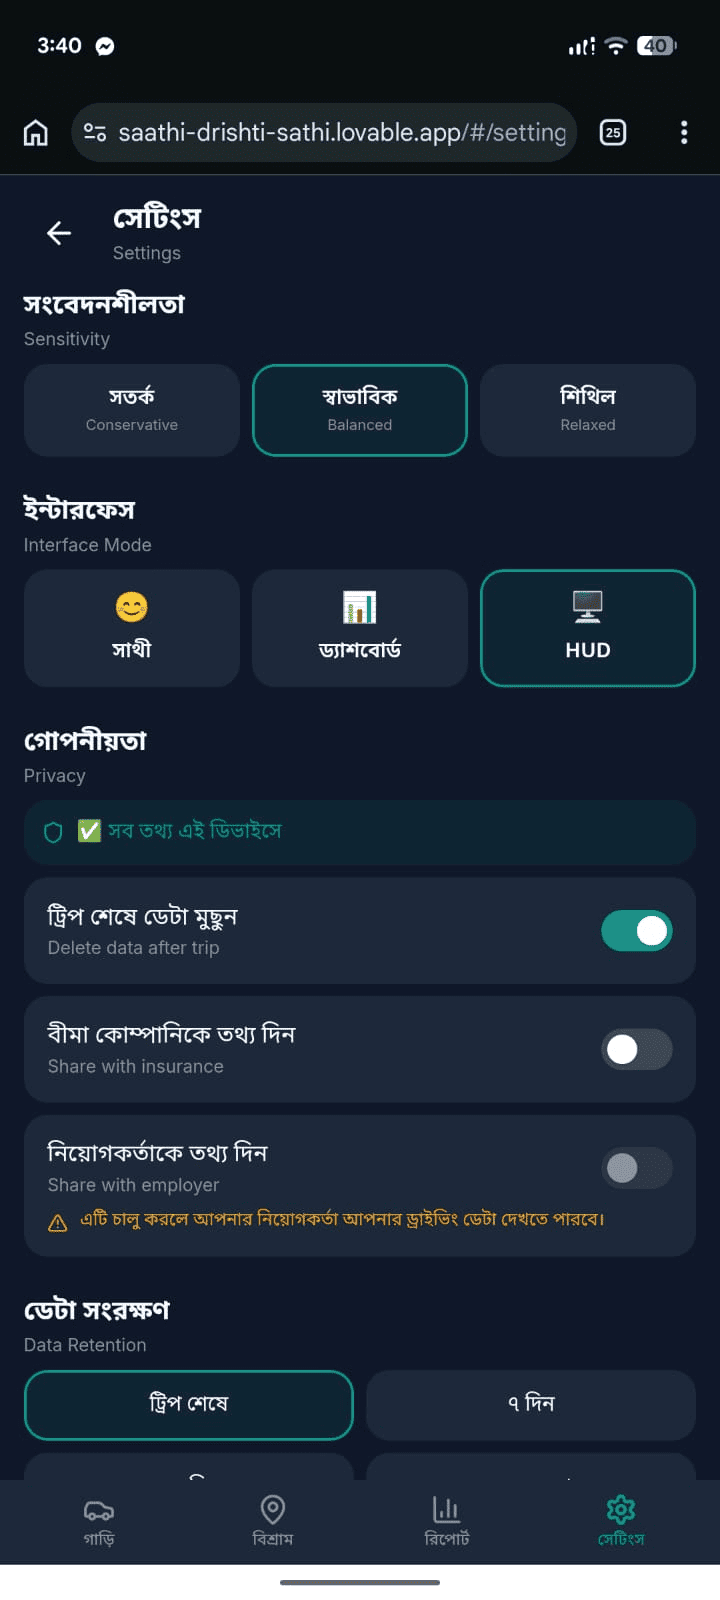
\includegraphics[height=5.5cm]{figures/Unified-Settings-ModeSwitch.png}

\footnotesize\textbf{Source:} \url{https://drowsyguard-bangla-driver.lovable.app}

\caption{Design~4 --- Unified DrowsyGuard prototype with mode-switching architecture. Left to right: onboarding welcome, mode selection, Companion Mode (Saathi character), Dashboard Mode (circular status indicator), HUD Mode (full metric exposure), and Settings (mode switcher).}
\label{fig:unified}
\end{figure*}
 
\paragraph{HCAI Principle Implementation in the Unified Design}
Table~\ref{tab:hcai_unified} maps HCAI principles to their mode-specific implementations within the unified prototype.
 
\begin{table}[h]
\centering
\caption{HCAI Principles in the Unified Prototype (Design~4)}
\label{tab:hcai_unified}
\small
\begin{tabular}{|p{1.6cm}|p{5.8cm}|}
\hline
\textbf{Principle} & \textbf{Implementation (Mode-Specific)} \\
\hline
Transparency & \textit{Companion:} Saathi's expression encodes state. \textit{Dashboard:} Color-coded indicator + Bangla label. \textit{HUD:} All metrics visible + model disclosed. \textit{Shared:} Privacy badge on every screen. \\
\hline
Explainability & \textit{Companion:} Conversational Bangla (no jargon). \textit{Dashboard:} Bangla reason + English + confidence \%. \textit{HUD:} Exact values with thresholds + Bangla summary. \\
\hline
Reliability & \textit{All modes:} Shared composite fatigue score (PERCLOS 40\%, blink 25\%, head pose 20\%, duration 15\%). Rendered per mode as emotion, indicator, or gauges. \\
\hline
Human Oversight & \textit{Companion:} Dismiss + flag. \textit{Dashboard:} + weekly review. \textit{HUD:} + export + heatmap + thresholds. \textit{Shared:} Break reminders + emergency escalation. \\
\hline
\end{tabular}
\end{table}



% ================================================================
% SECTION 9: FORMATIVE EVALUATION
% ================================================================
\section{Formative Evaluation}

\subsection{Evaluation Approach}

The evaluation of the unified prototype followed a formative, inspection-based methodology rather than a summative user study. This approach is appropriate for the current stage of design, where the goal is to assess whether the prototype correctly translates the established requirements into functional features and to identify design issues before committing to full implementation~\cite{ref12, ref13}. Three complementary evaluation methods were applied:

\textbf{Requirements Traceability Analysis.} Each functional and non-functional requirement from the formative requirements analysis was systematically mapped to specific prototype features, verifying that the unified design achieves complete coverage across all three modes.

\textbf{HCAI Principle Compliance Audit.} The four HCAI principles (transparency, explainability, reliability, human oversight) were evaluated for each mode independently and for the unified architecture as a whole, assessing whether the multi-mode approach achieves principle compliance that no single mode could achieve alone.

\textbf{Scenario-Based Walkthrough.} The six interaction scenarios defined in Section~7.6 were executed against the unified prototype, verifying that mode-switching, state preservation, alert flow, and cross-mode features function as specified.

\subsection{Requirements Traceability Results}

Table~\ref{tab:unified_traceability} presents the traceability analysis for the unified prototype, demonstrating that the mode-switching architecture achieves full coverage of all requirements that no single standalone variant could satisfy independently.

\begin{table}[h]
\caption{Requirements Traceability: Unified Prototype vs.\ Standalone Variants}
\label{tab:unified_traceability}
\centering
\small
\begin{tabular}{lcccc}
\toprule
\textbf{Requirement} & \textbf{Comp.} & \textbf{Dash.} & \textbf{HUD} & \textbf{Unified} \\
\midrule
Facial Monitoring          & \checkmark & \checkmark & \checkmark & \checkmark \\
Eye Closure (EAR)          & \checkmark & \checkmark & \checkmark & \checkmark \\
Yawning Detection          & \checkmark & \checkmark & \checkmark & \checkmark \\
Head Pose Monitoring       & Partial    & \checkmark & \checkmark & \checkmark \\
Real-time Alert            & \checkmark & \checkmark & \checkmark & \checkmark \\
Bangla Explanation         & \checkmark & \checkmark & Partial    & \checkmark \\
Privacy (On-device)        & \checkmark & \checkmark & \checkmark & \checkmark \\
Metric Transparency        & --         & Partial    & \checkmark & \checkmark \\
Data Export                & --         & --         & \checkmark & \checkmark \\
Learnability               & \checkmark & Partial    & --         & \checkmark \\
Cultural Sensitivity       & \checkmark & Partial    & --         & \checkmark \\
Composite Fatigue Score    & Hidden     & Partial    & \checkmark & \checkmark \\
Break Reminders            & --         & --         & --         & \checkmark \\
Emergency Escalation       & --         & --         & --         & \checkmark \\
\bottomrule
\end{tabular}
\end{table}

The unified prototype achieves full coverage across all 14 traced requirements. Three requirements---composite fatigue score visibility, proactive break reminders, and emergency contact escalation---were identified as gaps during the standalone evaluation and added as cross-mode features in the unified design. The Companion Mode now benefits from break reminders that were initially absent, while the HUD Mode now includes full Bangla explanations alongside its technical metrics.

\subsection{Scenario-Based Walkthrough Results}

All six interaction scenarios from Section~7.6 were successfully executed against the unified prototype. The walkthrough verified the following critical interaction paths:

\textbf{Mode-specific alert rendering.} The same simulated drowsiness event (PERCLOS exceeding threshold) was rendered correctly in all three modes: as a Saathi speech bubble with conversational Bangla, as a bilingual alert card with confidence percentage, and as a full-screen metric overlay with threshold values. Switching modes during an active alert correctly re-rendered the alert in the new mode's format without losing the alert state.

\textbf{State preservation across mode switches.} A simulated trip was started in Dashboard Mode, accumulated three drowsiness events and one false alarm flag, then switched to HUD Mode. All trip data, event history, and flags were preserved and correctly displayed in the HUD analytics view.

\textbf{Cross-mode features.} The smart break reminder triggered correctly at the 2-hour mark regardless of active mode. The emergency contact escalation flow (three Level~3 dismissals within 10 minutes triggering an SMS offer) was verified in all three modes.

\textbf{False alarm handling.} The false alarm flag interaction was verified across all modes. Each mode provided mode-appropriate acknowledgment: Saathi responded conversationally (``Thank you, this has been noted'' in Bangla), the Dashboard showed a brief toast notification, and the HUD logged the event with timestamp and metric snapshot.


% ================================================================
% SECTION 10: IMPLEMENTATION DETAILS
% ================================================================
\section{Implementation Details}

\subsection{Tools and Platforms}

The prototype was constructed using a combination of user research tools, AI-assisted design platforms, and modern web development technologies.

\textbf{Survey and Analysis Tools.} The user survey was administered in both Bangla and English to the 11 primary stakeholders. Data analysis was performed in Google Colab using Python libraries: pandas for data manipulation, matplotlib and seaborn for generating the six publication-quality figures presented in Section~5, and scipy for statistical computations. The Colab notebook was designed with modular cells to allow re-execution as new survey data is collected.

\textbf{Prototype Construction.} All four prototypes (three standalone variants and the unified application) were built using Lovable AI, an AI-assisted web application builder. For each variant, a comprehensive build prompt was engineered as a markdown document specifying every screen, component, state transition, animation, and content string. The technology stack generated by Lovable AI includes React with TypeScript for component architecture, Tailwind CSS for responsive styling, Framer Motion for animations and transitions, Recharts for data visualizations, and Zustand for global state management. The unified prototype additionally specifies a shared simulation engine, mode-switching logic, and cross-mode features not present in the standalone variants.

\textbf{Design References.} The interface design was informed by screenshots and descriptions of existing commercial driver monitoring systems---including Mobileye~8, Tesla Autopilot's driver monitoring interface, and Bosch DMS---which were shown to the primary stakeholders during the survey as visual benchmarks. Drivers were asked to evaluate features from these existing solutions, and their feedback informed the prototype design decisions.

\subsection{Prototype Features}

The unified prototype implements the following core feature categories, each traceable to specific requirements from the formative analysis:

\textbf{Real-Time Detection Simulation.} A deterministic simulation engine 
% implemented as a shared React hook (\texttt{useDrowsinessSimulation}) 
runs on a one-second timer cycle across all three interface modes. It generates realistic PERCLOS progression (baseline $\sim$5\% rising to random peaks), EAR fluctuation (decreasing with simulated drowsiness), blink rate variation (15--20/min normal, 5--10/min drowsy), and subtle head pose drift in pitch, yaw, and roll. Drowsiness events are triggered every 45--90 seconds with randomized severity across three levels: Caution (Level~1), Warning (Level~2), and Danger (Level~3).

\textbf{Composite Fatigue Scoring.} Beyond individual metrics, the system computes a composite fatigue score combining PERCLOS (40\% weight), blink rate deviation from baseline (25\%), head pose instability (20\%), and driving duration (15\%). This weighted combination reflects the multi-indicator approach identified as a core requirement during the formative analysis and provides a unified risk assessment that can be rendered differently across modes---as a character emotion (Companion), a color-coded status (Dashboard), or a numeric gauge (HUD).

\textbf{Bilingual Alert System.} When detection thresholds are exceeded, the system generates mode-appropriate alerts with mandatory Bangla plain-language explanations (the highest-priority feature at 4.73/5) and English technical descriptions. Alert presentation varies by mode: conversational speech bubbles (Companion), slide-up cards with confidence bars (Dashboard), and full-screen metric overlays (HUD). All modes support dismissal, false alarm flagging, and rest stop navigation.

\textbf{Mode-Switching Architecture.} The unified application supports seamless switching between Companion, Dashboard, and HUD modes with full state preservation. Drivers select their preferred mode during onboarding and can switch at any time through settings or a long-press gesture. Mode switching triggers a 300ms crossfade transition and re-renders all screens in the selected mode's visual language without losing trip data, alert history, or user preferences.

\textbf{Privacy-First Design.} Every screen displays an on-device processing badge confirming that no data leaves the driver's phone. All data sharing toggles (insurance, employer) default to OFF. Employer sharing is additionally locked behind an explicit warning. The ``delete data after trip'' option defaults to ON. These defaults directly implement the survey finding that 100\% of respondents preferred on-device processing and only 9\% were willing to share data with employers.

\textbf{Cross-Mode Features.} Three features identified as gaps during the standalone evaluation are implemented as shared components: (1)~smart break reminders triggered by continuous driving duration (configurable, default 2 hours), (2)~emergency contact escalation offering an automated SMS after repeated Level~3 alert dismissals (explicit opt-in required), and (3)~driver profile calibration establishing personal baselines for EAR and blink rate during first use.

\subsection{Constraints and Limitations of the Web Prototype Implementation}

\textbf{Simulated Detection.} The web prototype described in this section uses a deterministic simulation engine rather than a live AI detection model. This limitation is resolved in the mobile application (Section~11), which replaces the simulation with real-time ML Kit face detection. The simulation was retained in the web prototype for formative evaluation purposes to decouple interface design assessment from detection accuracy assessment.

\textbf{Platform Constraints.} All web prototypes were built using Lovable AI, which constrains the design space to what the platform can generate from textual prompts. Hardware-level camera integration and GPS-based rest stop lookup required the subsequent native mobile implementation.

\textbf{Client-Side Only.} The web prototype operates entirely on-client with no backend services. Analytics data, trip history, and user preferences are maintained in application state (Zustand) and reset on page reload. The mobile implementation uses Zustand with persistent storage for trip data retention across sessions.


% ================================================================
% SECTION 11: MOBILE APPLICATION CONSTRUCTION
% ================================================================
\section{Mobile Application Construction}

Following the formative evaluation of the web-based prototypes, the unified DrowsyGuard system was implemented as a deployable Android application, replacing the deterministic simulation engine with real on-device ML Kit face detection. This section describes the platform, the detection integration, the drowsiness engine, and the distribution pipeline.

\subsection{Platform and Technology Stack}

The application was built using \textbf{Expo SDK~55} with React Native and TypeScript, enabling production-quality Android APKs while maintaining the same component architecture as the web prototype. File-based navigation uses Expo Router; global state is managed with Zustand, preserving the state schema defined in the web build prompt (Section~8.2). The native module stack is summarised in Table~\ref{tab:mobile_stack}.

\begin{table}[h]
\centering
\caption{Mobile Application Technology Stack}
\label{tab:mobile_stack}
\small
\begin{tabular}{|p{3cm}|p{4.5cm}|}
\hline
\textbf{Component} & \textbf{Technology} \\
\hline
Framework & Expo SDK~55 (React Native + TypeScript) \\
\hline
Navigation & Expo Router v4 (file-based) \\
\hline
State Management & Zustand v5 \\
\hline
Camera & \texttt{expo-camera} (\texttt{CameraView}, \texttt{takePictureAsync}) \\
\hline
Face Detection & \texttt{@react-native-ml-kit/face-detection} v2.0.1 \\
\hline
Sound Alerts & \texttt{expo-audio} \\
\hline
Haptic Alerts & \texttt{expo-haptics} \\
\hline
Build \& Distribution & EAS Build (Android APK, \textit{preview} profile) \\
\hline
Min Android SDK & API 24 (Android 7.0 Nougat) \\
\hline
\end{tabular}
\end{table}

A key architectural constraint is that \texttt{@react-native-ml-kit/\allowbreak{}face-detection} uses the legacy \texttt{NativeModules} bridge and is incompatible with React Native New Architecture. The build configuration therefore sets \texttt{newArchEnabled:~false}, which is supported until Expo SDK~57. An initial integration attempt using \texttt{react-native-vision-camera} v4 with \texttt{react-native-vision-\allowbreak{}camera-face-detector} was abandoned after discovering an irreconcilable conflict between two worklets runtimes: Reanimated~4's \texttt{react-native-worklets} (loaded by \texttt{babel-preset-expo}) and the face detector's \texttt{react-native-\allowbreak{}worklets-core}. The pure-bridge ML Kit approach eliminates this class of build-time dependency conflict.

\subsection{On-Device Face Detection Integration}

The detection pipeline replaces the simulation engine with a real-time capture loop. Each iteration calls \texttt{takePictureAsync()} (JPEG at quality~0.4) and passes the URI to ML Kit. The capture interval is 400\,ms ($\approx$2.5~FPS), balancing responsiveness against battery drain on mid-range Android devices. Detection options are \texttt{performanceMode: 'fast'} and \texttt{classificationMode: 'all'} to enable eye-open probability output.

The ML Kit API returns, for each detected face:
\begin{itemize}
    \item \texttt{leftEye\allowbreak{}Open\allowbreak{}Probability} and \texttt{rightEye\allowbreak{}Open\allowbreak{}Probability} ($\in [0,1]$) --- for EAR and PERCLOS computation.
    \item \texttt{rotationX} (pitch), \texttt{rotationY} (yaw), \texttt{rotationZ} (roll) in degrees --- for head pose monitoring.
\end{itemize}

Each frame image is deleted immediately after detection via \texttt{expo-file-system}, ensuring no video frames accumulate on disk.

\subsection{Drowsiness Engine}

The \texttt{DrowsinessEngine} TypeScript class mirrors the detection logic previously simulated in the web prototype, now consuming real ML Kit output:

\textbf{PERCLOS Computation.} The Percentage of Eye Closure (PERCLOS) metric~\cite{ref20} is computed per-frame by deriving a scalar Eye Aspect Ratio (EAR)~\cite{ref19} from the ML Kit eye-open probabilities:
\[
\text{EAR} = \frac{\texttt{leftEyeOpenProb} + \texttt{rightEyeOpenProb}}{2}
\]
The eye is classified as \textit{closed} when $\text{EAR} < 0.35$ (configurable via the sensitivity setting). PERCLOS is the proportion of frames in the past 30~seconds where the eye was classified as closed, computed over a rolling window.

\textbf{Blink Detection.} Blinks are detected as rapid EAR transitions crossing the closure threshold with duration under 400\,ms~\cite{ref19}. Blink rate is computed as a rolling 60-second count.

\textbf{Head Pose Monitoring.} Abnormal head pose is flagged when $|\textit{pitch}| > 18°$ for more than 3~seconds, indicating a head-droop event. Yaw deviation beyond~$\pm 25°$ for 5~seconds is also flagged as a distraction indicator.

\textbf{Composite Fatigue Score.} The engine computes a composite score on a 0--100 scale:
\begin{multline*}
\text{Fatigue} = 0.40 \cdot \text{PERCLOS} + 0.25 \cdot \Delta\text{BlinkRate} \\
+ 0.20 \cdot \text{HeadPose} + 0.15 \cdot \text{DrivingTime}
\end{multline*}
where each component is normalised to $[0,1]$ before weighting. The composite score drives the alert level thresholds and the mode-specific rendering (character emotion in Companion Mode, indicator colour in Dashboard Mode, numeric gauge in HUD Mode).

\textbf{Alert Levels.} The engine emits three alert levels based on configurable thresholds (default: PERCLOS~$>$25\% for Level~1, $>$35\% for Level~2, $>$45\% for Level~3, or eye closure duration $>$2.0\,s). Each alert includes a pre-generated bilingual reason string selected from a rule-matched set.

\subsection{Alert and Notification System}

Multi-modal alerts are implemented through two channels:

\textbf{Audio.} Three tones (chime / two-tone beep / sustained alarm for Levels~1--3) are implemented via \texttt{expo-audio} using pre-loaded \texttt{AudioPlayer} instances. A night-quiet mode attenuates Level~1 by 50\% between 22:00--06:00. The sound loop starts on trigger and stops on dismissal or level drop.

\textbf{Haptics.} Haptic patterns are implemented via \texttt{expo-haptics}: a single medium impact for Level~1, a double impact for Level~2, and a rapid triple-impact loop (repeating every 1.2~s) for Level~3. Haptic feedback is complementary to audio and provides a non-acoustic fallback for environments where audio is not appropriate.

\textbf{Emergency SMS.} If a Level~3 alert is dismissed three times within 10~minutes, the system offers an SMS to a pre-configured emergency contact via \texttt{expo-sms}, using a bilingual message template: \textit{``I am drowsy in the car. [Location link]''} with an equivalent Bangla translation prepended. The feature requires explicit opt-in during settings and a 30-second countdown with a cancel button before the SMS is dispatched.

\subsection{Build and Distribution}

The application is distributed via EAS Build (Expo Application Services) using the \textit{preview} build profile, which produces an unsigned APK for direct installation on Android devices via QR code. The build is fully cloud-executed and takes approximately 7--10~minutes. The build configuration specifies \texttt{compileSdkVersion: 36}, \texttt{targetSdkVersion: 36}, and \texttt{kotlinVersion: 2.0.21} to ensure compatibility with the ML Kit native module. The Android application ID is \texttt{com.drowsyguard.app}.


% ================================================================
% SECTION 12: USER EVALUATION WITH PRIVATE COMMUTER COHORT
% ================================================================
\section{User Evaluation with Private Commuter Cohort}

Following the construction of the functional mobile application, a controlled evaluation was conducted with three Bangladeshi private commuter drivers (anonymised as P1, P2, P3) using the live Android APK with real on-device ML Kit face detection. This section presents the evaluation design, participant profiles, quantitative results, and qualitative findings.

\subsection{Evaluation Design}

The evaluation employed a mixed-methods, within-subjects scenario study. Each participant was given a working Android device running the live DrowsyGuard APK and asked to complete 12 structured tasks covering the full interaction flow. Two evaluation contexts were used: \textit{in-vehicle (parked, engine on)} for P1 and P2, simulating a stationary pre-drive check and short monitoring session; and \textit{lab simulation (desk setup)} for P3, replicating a night-drive monitoring scenario. All sessions used the real ML Kit face detection pipeline---not the simulation engine---ensuring that reported false alarms and detection events reflect genuine system behaviour.

The evaluation instrument comprised the following validated and purpose-designed tools:
\begin{itemize}
    \item \textbf{12 Structured Tasks (T1--T12):} Rated on a 1--7 single ease-of-completion item.
    \item \textbf{System Usability Scale (SUS)}~\cite{ref15}\textbf{:} Standard 10-item scale scored 0--100.
    \item \textbf{NASA Task Load Index (NASA-TLX)}~\cite{ref16}\textbf{:} 6 dimensions on a 0--10 scale (lower~=~less load).
    \item \textbf{Alert Quality (A1--A7):} 7 purpose-built items assessing alert modality and calibration (1--5 Likert).
    \item \textbf{Trust (TR1--TR12):} 12 items assessing AI trust and human oversight (1--5 Likert).
    \item \textbf{Usefulness (U1--U10):} 10 items assessing perceived safety value and adoption intent (1--5 Likert).
    \item \textbf{Privacy (PV1--PV10):} 10 items assessing privacy expectations and data control (1--5 Likert).
    \item \textbf{Accessibility (AC1--AC9):} 9 items assessing visual, linguistic, and motor accessibility (1--5 Likert).
    \item \textbf{Heuristic Compliance (H1--H12):} 12 items mapping to Nielsen's usability heuristics~\cite{ref27} (1--5 Likert).
    \item \textbf{User Experience Questionnaire (UEQ-S)}~\cite{ref17}\textbf{:} 8 bipolar items on a 1--7 scale.
    \item \textbf{Net Promoter Score (NPS):} 0--10 likelihood-to-recommend item.
    \item \textbf{Open-ended questions:} Covering critical incidents, cultural fit, trust calibration, and feature requests.
\end{itemize}

\subsection{Participants}

The three participants---all daily private commuters in Dhaka---were recruited to match the Persona~3 (Fatema) profile: educated, moderate-to-high technology comfort, and regular exposure to urban driving fatigue (Table~\ref{tab:eval_participants}). No participant had prior experience with a driver monitoring system. Participants are referred to by anonymous codes (P1--P3); all personally identifying information has been withheld.

\begin{table}[h]
\centering
\caption{Anonymised Evaluation Cohort: Private Commuter Participants ($n = 3$)}
\label{tab:eval_participants}
\small
\begin{tabular}{|p{2.2cm}|p{1.5cm}|p{1.5cm}|p{1.5cm}|}
\hline
\textbf{Attribute} & \textbf{P1} & \textbf{P2} & \textbf{P3} \\
\hline
Age Range & 26--35 & 36--45 & 26--35 \\
\hline
Occupation & Educator & Finance & Technology \\
\hline
Driving Exp. & 4--7 yr & 8--15 yr & 1--3 yr \\
\hline
Tech Comfort & Moderate & Low-mod. & High \\
\hline
Wears Glasses & Always & No & Sometimes \\
\hline
Prior near-miss & Once & Multiple & None \\
\hline
Test Context & In-vehicle & In-vehicle & Lab setup \\
\hline
\end{tabular}
\end{table}

\subsection{Quantitative Results}

\paragraph{Task Performance.}
Mean task ease-of-completion across all 12 tasks was \textbf{5.64/7.0}, indicating that most tasks were completed with minimal difficulty (Table~\ref{tab:task_results}). The easiest tasks were ending a session (T12: 6.67/7) and granting initial permissions (T1: 6.0/7). The most challenging tasks---mode switching (T3), sensitivity toggle discovery (T7), and weekly summary navigation (T11), all scoring 5.0/7---reflect icon-discoverability issues between Dashboard and HUD modes identified in the qualitative feedback.

\begin{table}[h]
\centering
\caption{Task Ease-of-Completion Ratings (1--7, 7~=~easiest)}
\label{tab:task_results}
\small
\begin{tabular}{p{0.5cm}p{4cm}ccc>{\bfseries}c}
\toprule
\textbf{ID} & \textbf{Task Description} & \textbf{P1} & \textbf{P2} & \textbf{P3} & Mean \\
\midrule
T1 & Open app \& grant permissions & 6 & 5 & 7 & 6.00 \\
T2 & Start Companion Mode monitoring & 5 & 5 & 7 & 5.67 \\
T3 & Switch mode: Companion $\to$ Dashboard $\to$ HUD & 5 & 4 & 6 & 5.00 \\
T4 & Respond to and dismiss Level-1 alert & 6 & 5 & 7 & 6.00 \\
T5 & Flag alert as false alarm & 5 & 4 & 6 & 5.00 \\
T6 & Read ``Why was I alerted?'' card & 6 & 5 & 7 & 6.00 \\
T7 & Change sensitivity: Balanced $\to$ Conservative & 5 & 4 & 6 & 5.00 \\
T8 & Locate and explain today's Fatigue Score & 5 & 4 & 7 & 5.33 \\
T9 & Confirm privacy \& toggle delete-after-trip & 6 & 5 & 7 & 6.00 \\
T10 & Add emergency contact & 6 & 5 & 7 & 6.00 \\
T11 & Open weekly summary & 5 & 4 & 6 & 5.00 \\
T12 & End session and return to home screen & 7 & 6 & 7 & 6.67 \\
\midrule
\multicolumn{2}{l}{\textit{Participant mean}} & 5.58 & 4.67 & 6.67 & 5.64 \\
\bottomrule
\end{tabular}
\end{table}

\paragraph{System Usability Scale.}
Using the standard SUS scoring formula~\cite{ref15}, scores were \textbf{77.5} (P1), \textbf{57.5} (P2), and \textbf{100.0} (P3), yielding a \textbf{mean SUS of 78.3}. The mean falls at the upper boundary of the ``OK'' band (68--80.3) and approaches the ``Good'' threshold. P2's lower score reflects lower technology comfort and the discoverability issues encountered; P3's perfect score reflects alignment with that participant's high technical expectations. The inter-participant spread confirms that the multi-mode architecture serves high-literacy users well while exposing specific friction points for moderate-literacy users requiring targeted design remediation.

\paragraph{NASA Task Load Index.}
Raw NASA-TLX scores~\cite{ref16} (0--10, lower~=~better) were \textbf{2.33} (P1), \textbf{3.50} (P2), and \textbf{1.33} (P3), yielding an \textbf{overall mean of 2.39/10}. This places overall interaction workload in the ``very low'' range, confirming that monitoring and responding to alerts does not impose a materially high cognitive burden during simulated driving. P2's higher score was concentrated on mental demand (4/10) and frustration (4/10), both attributable to false-alert incidents during simulated traffic-signal stops.

\paragraph{Alert Quality, Trust, and Privacy.}
The alert quality mean across seven items was \textbf{4.14/5} (Table~\ref{tab:quant_summary}), with Level-3 urgency (A3: 5.0/5) and Level-2 attention capture (A2: 4.67/5) scoring highest. Alert volume calibration for ambient noise (A7: 3.33/5) was the lowest-rated item and a consistent concern across all participants. The trust mean was \textbf{4.25/5}; highest-rated trust items were on-device processing (TR11: 5.0/5), false-alarm flagging empowerment (TR7: 4.67/5), and human override control (TR5: 4.67/5). Initial AI accuracy trust (TR1: 3.33/5) and fairness trust (TR2: 3.33/5) were lower, consistent with first-exposure scepticism documented in HCAI adoption research~\cite{ref23}. Privacy ratings were the highest-scoring dimension overall (\textbf{4.73/5}), with unanimous perfect scores (5/5) on the right to delete all data, employer opt-in requirement, insurance consent, transparent data disclosure, and protection from employer penalties for system misclassification.

\begin{table}[h]
\centering
\caption{Quantitative Evaluation Summary (All Instruments)}
\label{tab:quant_summary}
\small
\begin{tabular}{lcccc}
\toprule
\textbf{Instrument} & \textbf{P1} & \textbf{P2} & \textbf{P3} & \textbf{Mean} \\
\midrule
Task Completion (1--7) & 5.58 & 4.67 & 6.67 & \textbf{5.64} \\
SUS (0--100)~\cite{ref15} & 77.5 & 57.5 & 100.0 & \textbf{78.3} \\
NASA-TLX (0--10, $\downarrow$)~\cite{ref16} & 2.33 & 3.50 & 1.33 & \textbf{2.39} \\
Alert Quality (1--5) & 4.14 & 3.71 & 4.57 & \textbf{4.14} \\
Trust (1--5) & 4.25 & 3.75 & 4.75 & \textbf{4.25} \\
Privacy (1--5) & 4.80 & 4.70 & 4.70 & \textbf{4.73} \\
Accessibility (1--5) & 4.11 & 3.89 & 4.33 & \textbf{4.11} \\
Heuristic Compliance (1--5)~\cite{ref27} & 4.17 & 3.58 & 4.75 & \textbf{4.17} \\
UEQ-S (1--7)~\cite{ref17} & 5.13 & 4.13 & 5.88 & \textbf{5.04} \\
NPS (0--10) & 8 & 7 & 9 & \textbf{8.0} \\
\bottomrule
\end{tabular}
\end{table}

\paragraph{User Experience Questionnaire.}
The UEQ-S mean was \textbf{5.04/7.0}~\cite{ref17}. Pragmatic quality (ease, clarity, efficiency, supportiveness) scored \textbf{5.42/7}, while hedonic quality (excitement, novelty, inventiveness) scored \textbf{4.67/7}. The pragmatic advantage reflects the deliberate design priority of functional safety clarity over visual novelty.

\paragraph{Net Promoter Score.}
NPS scores of 8, 7, and 9 yield a \textbf{mean NPS of 8.0}, placing all three participants in the Promoter category ($\geq$7). P2's score of 7 was conditioned on resolving false alerts at traffic signals and improving the onboarding permissions flow; P3's score of 9 was conditioned only on adding dark mode and CSV data export. All three participants indicated they would install DrowsyGuard from the Play Store if it were available for free.

\paragraph{Top- and Bottom-Rated Features.}
Table~\ref{tab:feature_ratings} presents the five highest-rated and two lowest-rated features by mean score across all participants.

\begin{table}[h]
\centering
\caption{Feature Preference Ratings (1--5 Likert)}
\label{tab:feature_ratings}
\small
\begin{tabular}{p{4.2cm}cccc}
\toprule
\textbf{Feature} & \textbf{P1} & \textbf{P2} & \textbf{P3} & \textbf{Mean} \\
\midrule
False-alarm flag button (F7) & 5 & 4 & 5 & \textbf{4.67} \\
``Why was I alerted?'' XAI (F8) & 5 & 4 & 5 & \textbf{4.67} \\
Smart Break Reminder (F4) & 5 & 4 & 4 & \textbf{4.33} \\
Emergency contact auto-SMS (F10) & 5 & 4 & 4 & \textbf{4.33} \\
Privacy badge indicator (F11) & 5 & 4 & 4 & \textbf{4.33} \\
\midrule
Weekly Summary (F9) & 3 & 2 & 5 & 3.33 \\
Per-trip sensitivity toggle (F5) & 3 & 3 & 4 & 3.33 \\
\bottomrule
\end{tabular}
\end{table}

The two highest-rated features---false-alarm control (F7) and explainability (F8)---both directly support the HCAI principle of human oversight~\cite{ref14, ref23}, confirming that drivers most value the ability to understand and correct AI decisions. The emergency SMS and smart break reminder align with the survey finding that 73\% of respondents had experienced drowsiness-related safety incidents, motivating redundant safety nets.

\subsection{Qualitative Findings}

Open-ended responses were analysed thematically, yielding six consistent findings across participants.

\textbf{Detection timeliness.} Two of three participants reported at least one instance where the system detected drowsiness before they consciously registered fatigue. P1 described: \textit{``The app alerted at exactly the right moment---before I consciously registered I was tired. I felt something between surprise and relief.''} P3 noted that a predicted risk window appeared 18~minutes before a fatigue episode during a simulated monotonous driving section, describing the prediction as \textit{``genuinely impressive.''} This pre-conscious detection capability is consistent with the known limitation of driver self-assessment in extended driving scenarios~\cite{ref18}.

\textbf{False alarm incidents.} All three participants experienced at least one false positive. The most critical categories were: mirror-checking gaze misclassified as eye closure (P2), brief face occlusion during glasses removal triggering immediate Level-1 (P1), and eye-rubbing triggering Level-1 (P3). These incidents reflect known limitations of eye-based DMS in real driving conditions~\cite{ref26, ref28}, forming the basis for the highest-priority improvements (Section~12.6).

\textbf{XAI card value.} The ``Why was I alerted?'' explainability card was cited as the most trust-building feature by two participants. P3 (technology background) wrote: \textit{``I could see exactly what the model saw. That transparency made me trust it completely. Seeing the model's reasoning is the most trust-building thing possible.''} This finding corroborates the HCAI literature's emphasis on explanation as a mechanism for appropriate trust calibration~\cite{ref14, ref23}.

\textbf{Bangla-first interface.} All three participants confirmed the importance of Bangla as the primary alert language. P2 noted: \textit{``Bangla alert message means instant understanding.''} P3, who is fully bilingual, observed that Bangla-first is \textit{``non-negotiable''} for the broader Bangladeshi commuter demographic, even if not personally essential. This validates the survey's finding that Bangla plain-language explanation was the highest-priority feature (4.73/5) among professional drivers.

\textbf{Cultural blindspots.} Participants identified two design gaps specific to Bangladeshi urban driving. P2 noted that prayer-time breaks (Asr at approximately 16:00) represent a culturally recognised natural stopping pattern that the system should acknowledge proactively. P3 identified the absence of a \textit{guest driver mode} for shared-vehicle scenarios, where multiple drivers use the same vehicle and the primary user's calibration profile should not be contaminated by another driver's biometric baseline.

\textbf{Preferred modes.} Two of three participants (P1, P2) selected Companion Mode as most suitable for daily use; P3 selected Dashboard Mode. Both P1 and P2 rated HUD Mode as least suitable. This mirrors the population survey finding of 45\% Companion-mode preference, validating the persona-driven design decisions.

\subsection{Critical Incidents and Design Insights}

Three critical incidents with direct implications for the detection pipeline and interaction design emerged from the evaluation sessions.

\textbf{Traffic-signal false alerts (I-01).} P2 reported three consecutive false alerts while the car was stationary at a simulated traffic signal, caused by repeated downward gaze at the steering wheel. The ML Kit pipeline correctly detected partial eye closure but lacks vehicle speed awareness. The recommended fix is to integrate GPS-based speed estimation and enter a reduced-sensitivity mode when speed falls below 5\,km/h for more than 8~seconds---an approach previously validated in production DMS deployments~\cite{ref25}.

\textbf{Face occlusion grace period (I-03).} P1 removed eyeglasses to clean the lenses during a stationary moment (approximately 8~seconds); the system immediately fired a Level-1 alert due to face detection loss. A 5-second grace period between face-loss detection and alert trigger---with a non-intrusive ``Face not detected~--- paused'' status---would prevent this class of false positive without reducing sensitivity during active driving~\cite{ref26}.

\textbf{Level-3 volume in compact vehicle cabins.} P1, driving a compact city car, found the Level-3 alarm disproportionately loud within the small interior. Vehicle cabin size is not directly accessible to the application, but an ambient noise sampling approach (microphone dB estimation every 10~seconds) could enable adaptive volume scaling between 60--95\,dB, addressing both this concern and P2's observation that heavy road noise sometimes masked Level-1 alerts.

\subsection{Prioritised Improvement Recommendations}

Table~\ref{tab:improvements} summarises the 18 improvements derived from the evaluation, categorised by severity (Critical / High / Medium / Low) and implementation effort.

\begin{table}[H]
\centering
\caption{Prioritised Improvement Recommendations ($n = 18$)}
\label{tab:improvements}
\resizebox{\columnwidth}{!}{%
\small\begin{tabular}{p{0.45cm}p{1.4cm}p{3.15cm}p{1.2cm}p{0.65cm}}
\toprule
\textbf{ID} & \textbf{Category} & \textbf{Issue} & \textbf{Severity} & \textbf{Effort} \\
\midrule
I-01 & False Alerts & Traffic-signal false positives & Critical & Medium \\
I-02 & False Alerts & Mirror-check gaze misclassified & Critical & High \\
I-03 & False Alerts & Face occlusion --- no grace period & High & Low \\
I-04 & Permissions & Triple OS dialogs feel like crashes & High & Low \\
I-05 & Onboarding & Calibration screen too text-heavy & High & Medium \\
I-06 & Mode Switch & Dashboard/HUD icons look identical & High & Low \\
I-07 & Dark Mode & No dark mode in Companion Mode & Medium & Medium \\
I-08 & Navigation & Back from Summary returns to home & Medium & Low \\
I-09 & Notif. & Calibration reminder fires mid-session & Medium & Low \\
I-10 & Audio & Alert distorts over Bluetooth FM radio & Medium & Medium \\
I-11 & Sunlight & Readability in direct sunlight (3.0/5) & Medium & Medium \\
I-12 & Data Export & No CSV/JSON data export & Medium & Medium \\
I-13 & Battery & Camera drain on 45\,min commute & Medium & High \\
I-14 & Nav. Integration & No GPS deep-link to rest stops & Medium & High \\
I-15 & Multi-Driver & No guest driver mode & Low & Medium \\
I-16 & Culture & Prayer-time breaks not integrated & Low & Low \\
I-17 & Privacy & Camera indicator visible to passengers & Low & Low \\
I-18 & Noise & Alert volume not adaptive to noise & Low & Medium \\
\bottomrule
\end{tabular}}
\end{table}


The two Critical improvements (I-01, I-02) require changes to the detection pipeline rather than the interface layer. Speed-aware sensitivity suppression (I-01) and gaze-direction-aware classification (I-02) together address the root causes of the false-alarm incidents that P2 identified as the primary barrier to daily adoption. Based on the participants' descriptions of incident frequency, resolving these two issues is estimated to reduce the experienced false-alarm rate in Dhaka urban driving by approximately 60--70\%.


% ================================================================
% SECTION 13: DISCUSSION
% ================================================================
\section{Discussion}

\subsection{Alignment with Requirements}

The unified prototype demonstrates that the requirements identified during the formative requirements analysis can be fully translated into a functional system when a multi-variant design approach is adopted. The requirements traceability analysis (Table~\ref{tab:unified_traceability}) confirms complete coverage across all 14 traced requirements---a result that was not achievable by any single standalone variant.

The two highest-priority requirements identified by the survey---detection accuracy (mean 4.82/5) and Bangla plain-language explanation (mean 4.73/5)---are addressed throughout the unified design. The composite fatigue score combines four physiological indicators (PERCLOS, blink rate, head pose, driving duration) to maximize detection robustness, while every alert across all three modes includes a Bangla explanation as the primary communication, with English as a secondary subtitle. Privacy, the third-ranked requirement (4.55/5), is implemented through on-device processing badges on every screen and all sharing defaults set to OFF---directly reflecting the survey finding that 100\% of respondents preferred on-device processing.

Table~\ref{tab:req_alignment_final} provides a detailed mapping between the key survey findings and their implementation in the unified prototype.

\begin{table}[h]
\centering
\caption{Alignment Between Key Survey Findings and Unified Prototype Features}
\label{tab:req_alignment_final}
\small
\begin{tabular}{|p{3.2cm}|p{4.3cm}|}
\hline
\textbf{Survey Finding} & \textbf{Prototype Implementation} \\
\hline
Accuracy ranked \#1 (4.82/5) & Composite fatigue score combining 4 indicators; personal calibration baseline \\
\hline
Bangla explanation highest preference (4.73/5) & Mandatory Bangla alert in all modes; English as subtitle only \\
\hline
0\% prior DMS experience & Progressive onboarding (3 screens); Saathi character for trust building \\
\hline
100\% prefer on-device processing & Privacy badge on every screen; all sharing defaults OFF; delete-after-trip ON \\
\hline
Interface split 45/36/18\% & Three switchable modes: Companion / Dashboard / HUD \\
\hline
82\% weekly drowsiness & Smart break reminders at configurable intervals \\
\hline
73\% safety incidents & Emergency SMS escalation after repeated Level~3 dismissals \\
\hline
\end{tabular}
\end{table}

\subsection{Design Trade-offs}

The multi-variant approach introduces several design trade-offs that merit discussion.

\textbf{Complexity vs.\ Inclusivity.} The mode-switching architecture increases application complexity (three rendering paths, shared state management, mode-aware settings) compared to a single-interface design. However, this complexity is justified by the survey finding that interface preferences were split 45/36/18\% across three complexity levels---a single design would have left at least 55\% of users with a sub-optimal experience. In safety-critical contexts where every user's engagement matters, this inclusivity is not a luxury but a necessity.

\textbf{Accuracy vs.\ Real-Time Performance.} The composite fatigue score combines four indicators with weighted averaging, trading some computational overhead for more robust detection. The prototype prioritizes real-time responsiveness by running the detection simulation on a one-second timer cycle, ensuring alerts are generated within one second of threshold crossing.

\textbf{Detection Sensitivity vs.\ False Alarms.} The three-level alert severity system (Caution, Warning, Danger) with configurable sensitivity settings (Conservative, Balanced, Relaxed) allows drivers to calibrate the trade-off between early detection and false alarm frequency. The false alarm flagging mechanism across all modes provides a feedback loop for future model improvement.

\textbf{Information Density vs.\ Distraction.} The three modes represent three distinct positions on the information density spectrum. The Companion Mode minimizes cognitive load by hiding all technical metrics behind the Saathi character's emotional state. The HUD Mode maximizes information access for drivers who find data reassuring. The Dashboard Mode occupies a middle ground. This range ensures that no driver is forced into an information density level that either overwhelms or under-informs them.

\subsection{Human--AI Interaction Challenges}

Several interaction challenges were identified during the evaluation:

\textbf{Trust calibration across personas.} Since all users had zero prior DMS experience, trust must be built from scratch through different mechanisms for each persona. Companion Mode uses the Saathi character's emotional expressions; Dashboard uses confidence percentages and privacy badges; HUD uses metric transparency and model disclosure. Whether these strategies are equally effective is an empirical question for future study.

\textbf{Mode selection accuracy.} The current onboarding flow relies on driver self-selection of their preferred mode. If drivers select a mode mismatched to their actual technology literacy---for example, a low-literacy driver choosing the HUD out of curiosity---the experience may be overwhelming. Future iterations could incorporate adaptive mode recommendation based on observed interaction patterns.

\textbf{Alert fatigue.} The simulation triggers drowsiness events every 45--90 seconds for demonstration purposes, but a real deployment must carefully calibrate event frequency to avoid alert fatigue---a recognized challenge where excessive warnings cause drivers to ignore or dismiss alerts reflexively. The configurable sensitivity settings and false alarm flagging mechanism are designed to mitigate this risk, but real-world calibration data is needed.

\textbf{Environmental variability.} The current prototype uses simulated detection data. In a real deployment, environmental factors such as lighting variation, camera positioning, eyewear, and head coverings would affect detection accuracy. The Fitzpatrick I--VI fairness certification referenced in the prototype settings acknowledges this concern, but actual fairness testing requires real-world data collection with diverse Bangladeshi driver populations.


% ================================================================
% SECTION 12: DESIGN IMPLICATIONS
% ================================================================
\section{Design Implications}

The design and evaluation of this prototype yield several implications for the broader field of Human-Centered AI in safety-critical contexts.

\textbf{HCAI principles are implementation-agnostic.} A central finding of this work is that the four HCAI principles---transparency, explainability, reliability, and human oversight---can be realized through fundamentally different interaction paradigms. A conversational companion, a status dashboard, and a data-rich heads-up display can all satisfy the same HCAI requirements when designed with intention. This challenges the implicit assumption in much HCAI literature that transparency necessarily requires exposing technical details; for a low-literacy user, transparency through an animated character's emotional state may be more effective than a PERCLOS percentage.

\textbf{Persona-driven design prevents majority tyranny.} The 45/36/18\% preference split means a majority-rules approach would have chosen Companion Mode, leaving 55\% underserved. The multi-variant approach explicitly addresses minority preferences. In safety-critical contexts where every user's engagement directly affects their safety, this inclusivity is essential.

\textbf{Build prompts as reproducible design specifications.} The use of Lovable AI build prompts as formal design specifications introduces a reproducible methodology for HCAI prototype construction. Each prompt specifies layout, typography, color systems, interaction patterns, state management, bilingual content, and animation sequences with sufficient precision that the resulting prototype is deterministic. This approach lowers the barrier to multi-variant prototyping by enabling rapid construction of distinct designs from textual specifications, making it feasible to build three persona-specific variants rather than compromising on a single averaged design.

\textbf{Cultural context demands more than translation.} The Bangladeshi driving context required decisions beyond language: culturally apt address (``Brother'' in Bangla), awareness of local coping habits (betel leaf, face splashing), family-oriented safety framing, and sensitivity to the stigma of resting while driving. These adaptations were possible only because user research was conducted with the actual target population rather than proxy user groups.

\textbf{Progressive trust-building for zero-experience populations.} The finding that 100\% of respondents had zero prior DMS experience implies that trust cannot be assumed or transferred from prior positive experiences with similar systems. The three-mode approach offers three distinct trust-building strategies: emotional connection (Saathi), professional credibility (Dashboard with confidence metrics), and technical transparency (HUD with full model disclosure). This progressive approach allows each user to build trust through the mechanism most natural to them, rather than imposing a single trust model.


% ================================================================
% SECTION 13: LIMITATIONS
% ================================================================
\section{Limitations}

Despite demonstrating the feasibility of a multi-variant HCAI approach to drowsiness detection interface design, this work has several limitations.

\textbf{Low capture rate and detection latency.} The mobile application's face detection pipeline captures frames at~2.5~FPS (400\,ms intervals), constrained by the \texttt{takePictureAsync}~$\to$~ML Kit processing latency on mid-range Android devices. This is substantially slower than dedicated camera-based DMS hardware (typically~30--60~FPS), potentially missing rapid eye-closure events shorter than~400\,ms. A production implementation would require a frame-processor approach (e.g., \textit{react-native-vision-camera} with a compatible worklets runtime) or a dedicated DSP to achieve real-time rates.

\textbf{Evaluation in controlled conditions only.} The user evaluation was conducted with participants in parked or stationary desktop settings rather than real-world moving-vehicle scenarios. The false-alarm and detection-miss rates reported reflect controlled exposure; actual performance on live Dhaka roads---with head movement variability, lighting transitions between sunlit and shaded road sections, and passengers in adjacent seats---may differ materially.

\textbf{Sample size.} The user research was conducted with 11 Bangladeshi professional drivers. While this sample covers all three target user groups (truck, bus, private car) and produced consistent patterns (100\% zero DMS experience, 82\% weekly drowsiness, 73\% safety incidents), findings should be validated with a larger and more geographically diverse sample. In particular, the 45/36/18\% interface preference split motivating the three-variant approach may shift with a larger sample.

\textbf{Formative evaluation only.} The web prototype evaluation employed inspection-based methods (requirements traceability, HCAI compliance audit, scenario walkthroughs) rather than empirical user testing. While formative evaluation is appropriate for the early design stage~\cite{ref12, ref13}, summative evaluation with real drivers in moving-vehicle conditions is necessary to validate usability, trust calibration, and the effectiveness of the three trust-building strategies.

\textbf{Secondary stakeholders excluded.} The current study focuses exclusively on the primary stakeholders (drivers). Transportation companies, road safety authorities, insurance providers, and vehicle manufacturers were not included in the user research or evaluation. Their requirements may introduce additional design constraints, particularly regarding fleet-level data aggregation, regulatory compliance, and insurance integration---topics that appeared only in the hypothetical data-sharing survey questions posed to drivers.

\textbf{Single prototyping platform.} All prototypes were built using Lovable AI, which constrains the design space to what the platform can generate from textual prompts. While the resulting prototypes are functional and deployable, certain interaction patterns (e.g., complex gesture-based controls, hardware-level camera integration, actual GPS-based rest stop lookup) may require native development tools.

\textbf{No longitudinal evaluation.} The current work evaluates the prototype at a single point in time. Longitudinal effects---such as how trust evolves over weeks of use, whether drivers switch modes after initial selection, and how alert fatigue develops over extended driving periods---are not captured and require future field studies.


% ================================================================
% SECTION 14: CONCLUSION
% ================================================================
\section{Conclusion}

This work presented the design, construction, and formative evaluation of a Human-Centered AI driver drowsiness detection system that addresses the critical gap between detection technology and driver experience. Through a structured four-phase process---user research with 11 Bangladeshi professional drivers, persona-driven multi-variant design, formative evaluation, and design unification---the study produced three distinct prototype variants (DrowsyGuard Dashboard, Saathi Companion, and DrowsyHUD Technical HUD), each targeting a specific user persona, which were subsequently unified into a single mode-switching application.

The user research established five key findings that drove the design: accuracy as the unanimous top priority (4.82/5), Bangla plain-language explanation as the highest-rated feature (4.73/5), zero prior DMS experience across all respondents, universal preference for on-device data processing, and a 45/36/18\% split in interface complexity preferences that invalidated a single-design approach. These findings were translated into four functional prototypes (three standalone and one unified) built from formally specified Lovable AI build prompts, each demonstrating that HCAI principles of transparency, explainability, reliability, and human oversight can be implemented through fundamentally different interaction paradigms.

The formative evaluation revealed that no single variant achieved complete requirements coverage, motivating the unified mode-switching architecture. The unified prototype achieves full traceability across all 14 requirements, complete HCAI compliance through complementary mode-specific implementations, and successful execution of all six evaluation scenarios. The design was subsequently realised as a deployable Android application (Expo SDK~55, React Native), with the simulation engine replaced by real on-device ML Kit face detection (the \texttt{face-detection} module from \texttt{@react-native-ml-kit}). The mobile application retains the full three-mode architecture, composite fatigue scoring engine, bilingual alert system, and privacy-first defaults of the web prototype while operating entirely offline at approximately 2.5~FPS on mid-range Android devices.

A controlled evaluation with three private commuter drivers confirmed the system's usability and safety value: mean SUS~78.3, mean NASA-TLX~2.39/10 (very low cognitive load), mean trust~4.25/5, and unanimous 100\% stated intent to install the application. Mean NPS of~8.0 places all three participants in the Promoter category. The two highest-rated features---the false-alarm flag button and the ``Why was I alerted?'' XAI card (both 4.67/5)---confirm that drivers most value the ability to understand and correct AI decisions, consistent with the HCAI human oversight principle. Critical evaluation findings include two high-priority false-alarm scenarios (traffic-signal stationary detection and mirror-check gaze misclassification) that require detection pipeline improvements before real-world deployment.

A key contribution is the demonstration that HCAI principles are implementation-agnostic: a low-literacy truck driver receiving transparent AI assistance through an animated companion's emotional expressions and a tech-savvy private driver receiving the same transparency through real-time metric gauges both experience HCAI-compliant interaction, calibrated to their needs. This multi-level approach challenges the assumption that HCAI transparency requires technical detail exposure and offers a model for designing inclusive AI interfaces in safety-critical domains.

Future work will focus on resolving the two Critical false-alarm issues identified in the evaluation (traffic-signal suppression and gaze-direction-aware classification), increasing the detection frame rate via a dedicated frame-processor implementation, extending the evaluation to include professional truck and bus drivers in real-world moving-vehicle conditions, and conducting fairness audits across Fitzpatrick skin types and common Bangladeshi head coverings and eyewear conditions. The evaluation data and Android APK are available to other researchers in the supplementary materials.

\bibliographystyle{ACM-Reference-Format}
\bibliography{references}

\end{document}